\documentclass[12pt]{extarticle}
\usepackage[paperwidth=18in,paperheight=7.5in]{geometry}
\usepackage{amsmath}
\usepackage{hyperref}
\usepackage{multirow}
\usepackage{pdfpages}
\usepackage[utf8]{inputenc}
\title{Kaon mixing: chiral and continuum extrapolations}
\author{R Mukherjee}
\date{\today}
\begin{document}
\maketitle
\tableofcontents
\clearpage
\begin{figure}
\centering
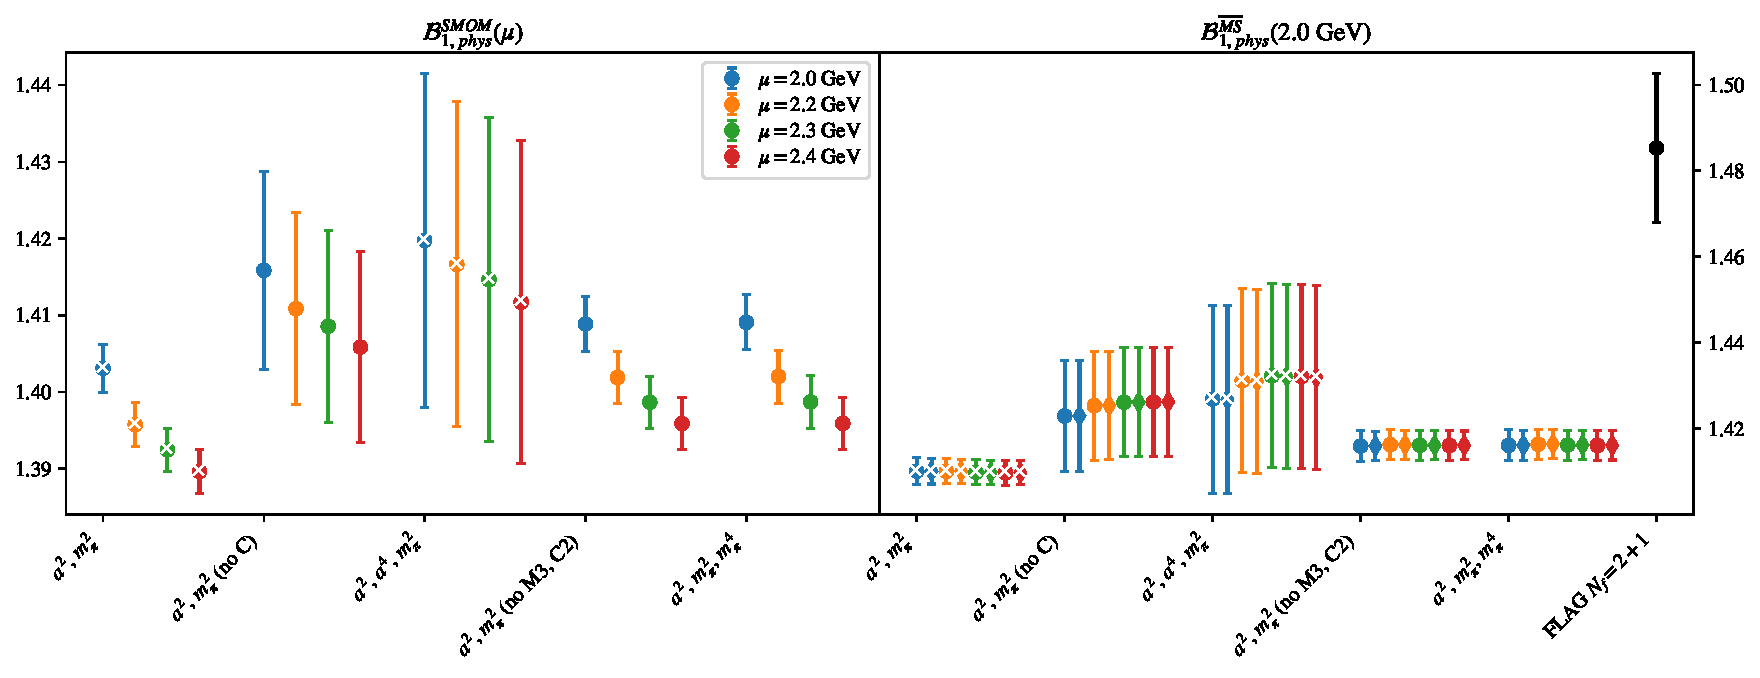
\includegraphics[page=1, width=1.1\textwidth]{VVpAA/SUSY/fit_summary_bag.pdf}
\caption{$\mathcal{B}_{1}$\\(left) $\mathcal{B}_{phys}$ in RI/SMOM scheme from fit variations (fits with $p$-value $<0.05$ marked with ``$\times$"). \\(right) $\mathcal{B}_{phys}$ in $\overline{MS}$ computed using $\mathcal{B}^{\overline{MS}} = R^{\overline{MS}\leftarrow SMOM}(2.0)\sigma_{npt}(2.0,\mu) \mathcal{B}^{SMOM}(\mu)$.}
\end{figure}
\clearpage
\begin{figure}
\centering
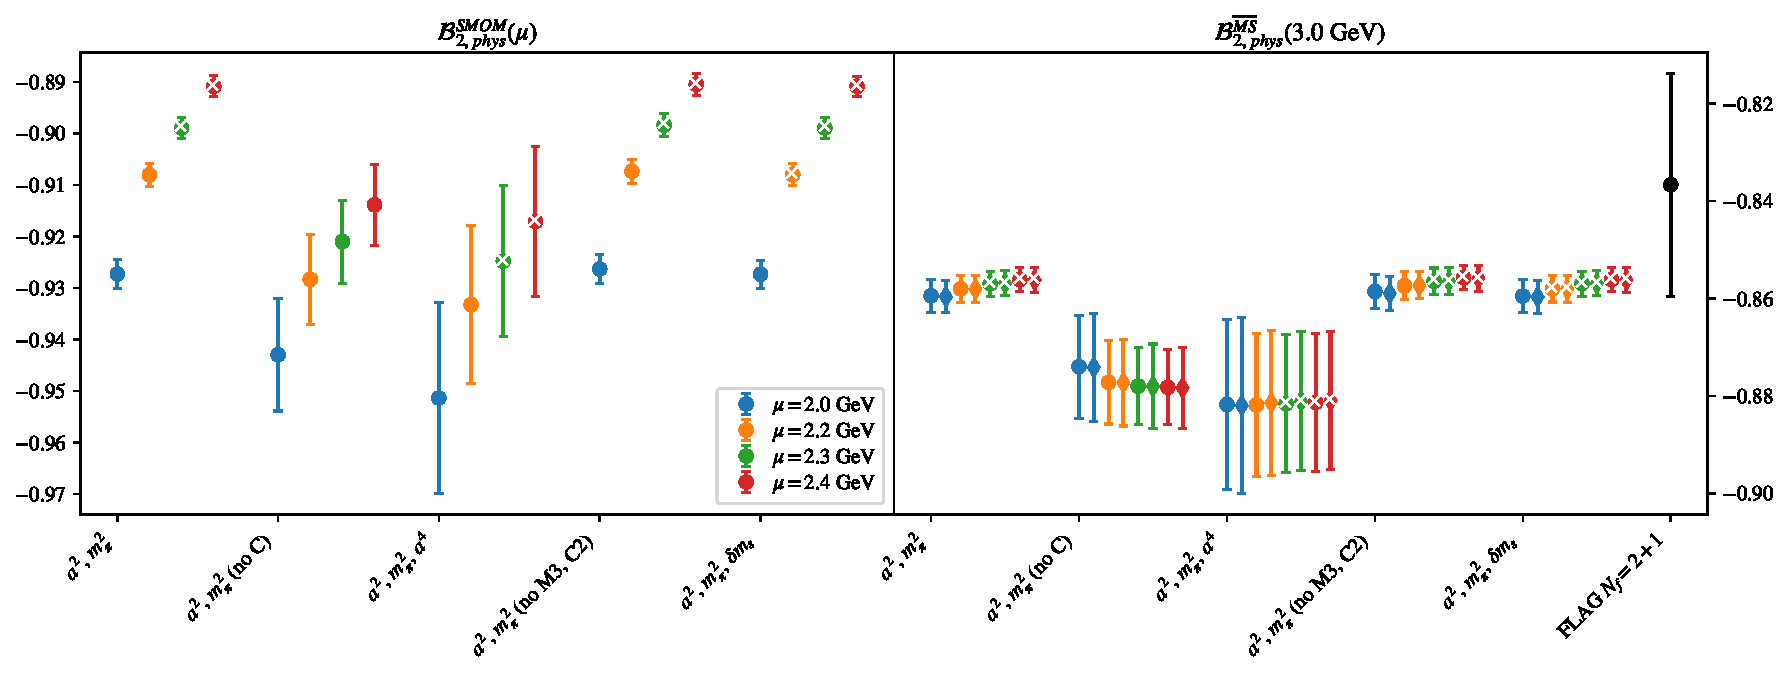
\includegraphics[page=1, width=1.1\textwidth]{VVmAA/SUSY/fit_summary_bag.pdf}
\caption{$\mathcal{B}_{2}$\\(left) $\mathcal{B}_{phys}$ in RI/SMOM scheme from fit variations (fits with $p$-value $<0.05$ marked with ``$\times$"). \\(right) $\mathcal{B}_{phys}$ in $\overline{MS}$ computed using $\mathcal{B}^{\overline{MS}} = R^{\overline{MS}\leftarrow SMOM}(3.0)\sigma_{npt}(3.0,\mu) \mathcal{B}^{SMOM}(\mu)$.}
\end{figure}
\clearpage
\begin{figure}
\centering
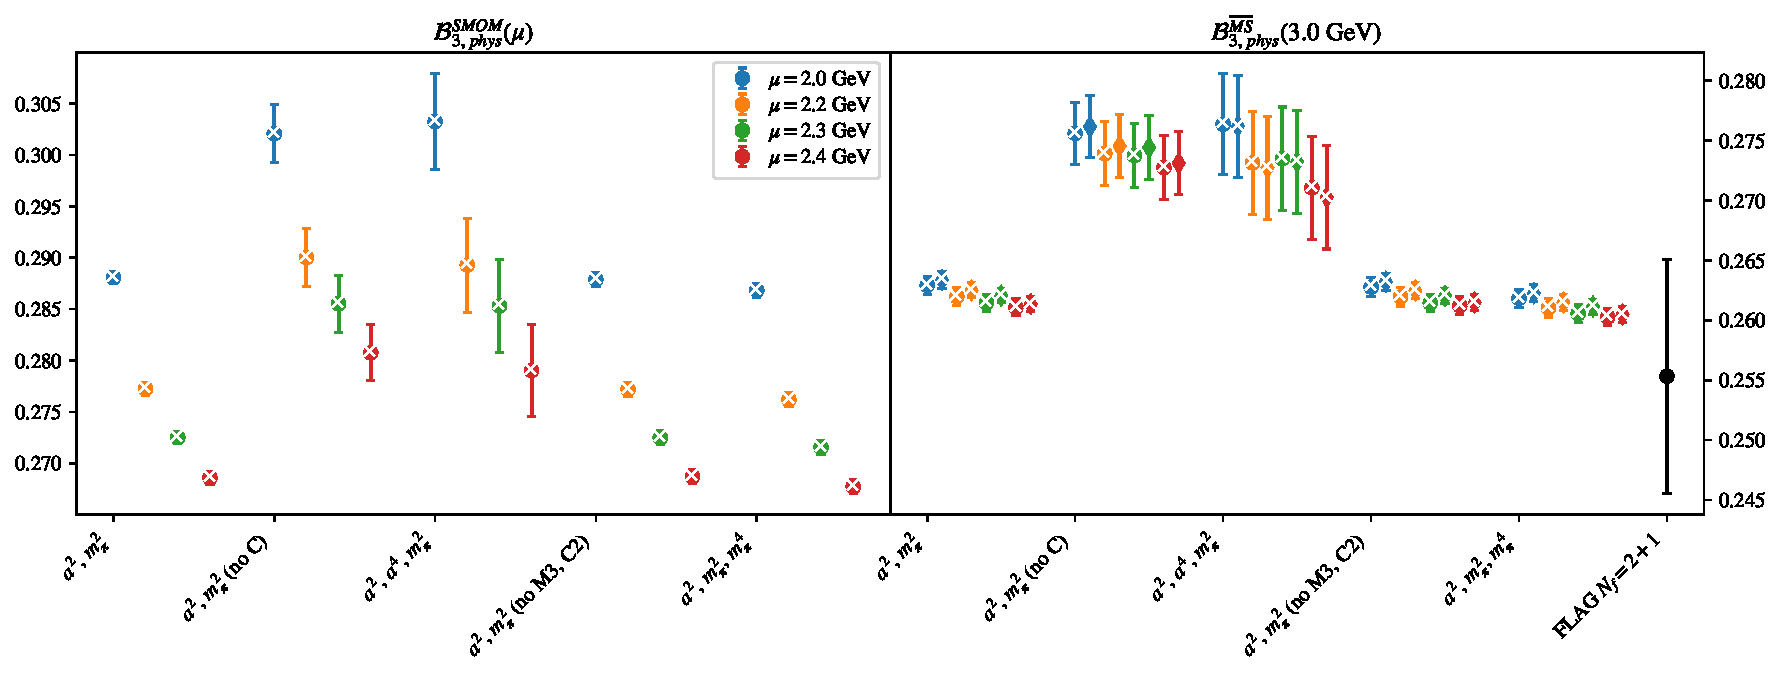
\includegraphics[page=1, width=1.1\textwidth]{SSmPP/SUSY/fit_summary_bag.pdf}
\caption{$\mathcal{B}_{3}$\\(left) $\mathcal{B}_{phys}$ in RI/SMOM scheme from fit variations (fits with $p$-value $<0.05$ marked with ``$\times$"). \\(right) $\mathcal{B}_{phys}$ in $\overline{MS}$ computed using $\mathcal{B}^{\overline{MS}} = R^{\overline{MS}\leftarrow SMOM}(3.0)\sigma_{npt}(3.0,\mu) \mathcal{B}^{SMOM}(\mu)$.}
\end{figure}
\clearpage
\begin{figure}
\centering
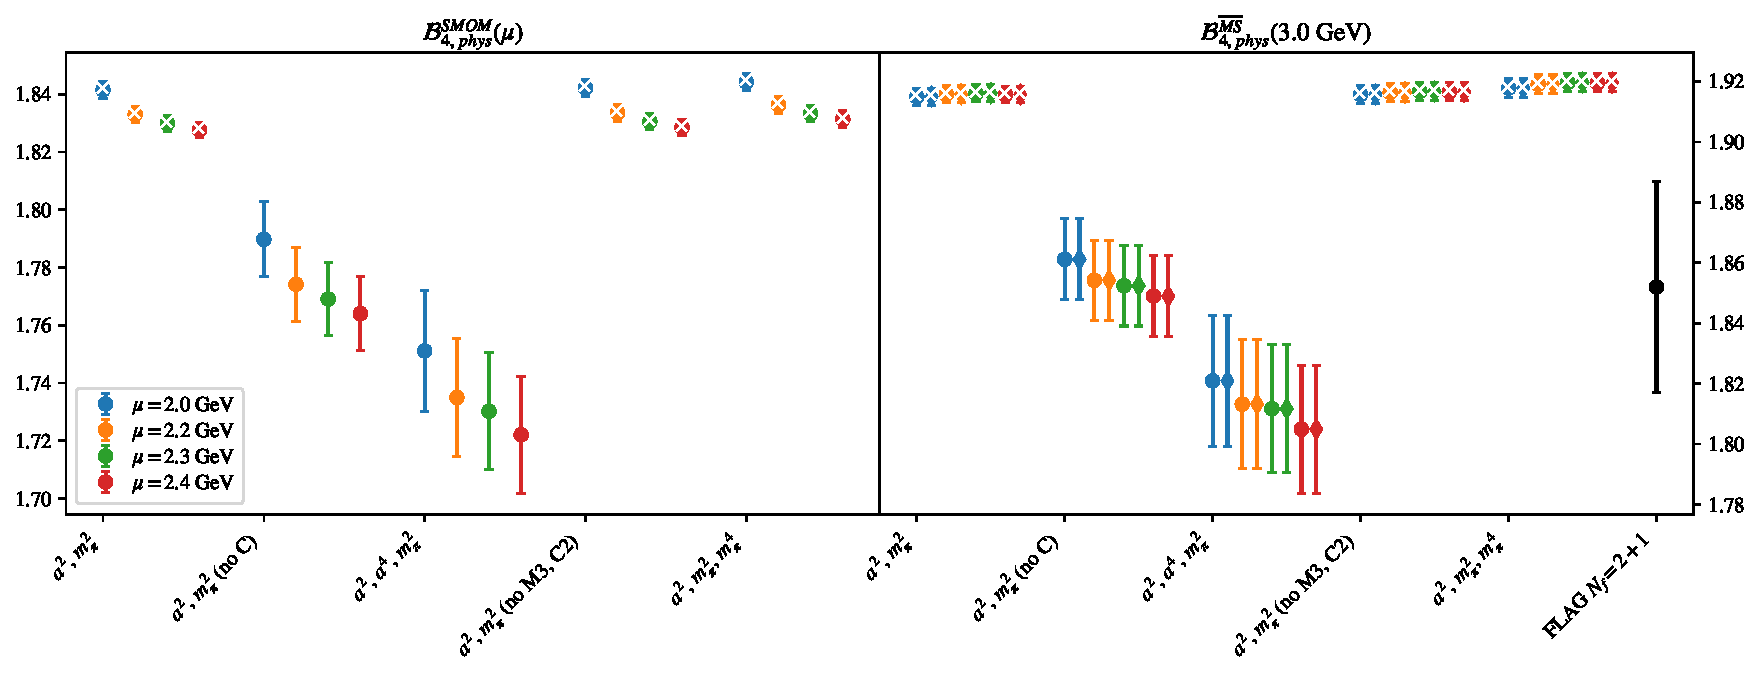
\includegraphics[page=1, width=1.1\textwidth]{SSpPP/SUSY/fit_summary_bag.pdf}
\caption{$\mathcal{B}_{4}$\\(left) $\mathcal{B}_{phys}$ in RI/SMOM scheme from fit variations (fits with $p$-value $<0.05$ marked with ``$\times$"). \\(right) $\mathcal{B}_{phys}$ in $\overline{MS}$ computed using $\mathcal{B}^{\overline{MS}} = R^{\overline{MS}\leftarrow SMOM}(3.0)\sigma_{npt}(3.0,\mu) \mathcal{B}^{SMOM}(\mu)$.}
\end{figure}
\clearpage
\begin{figure}
\centering
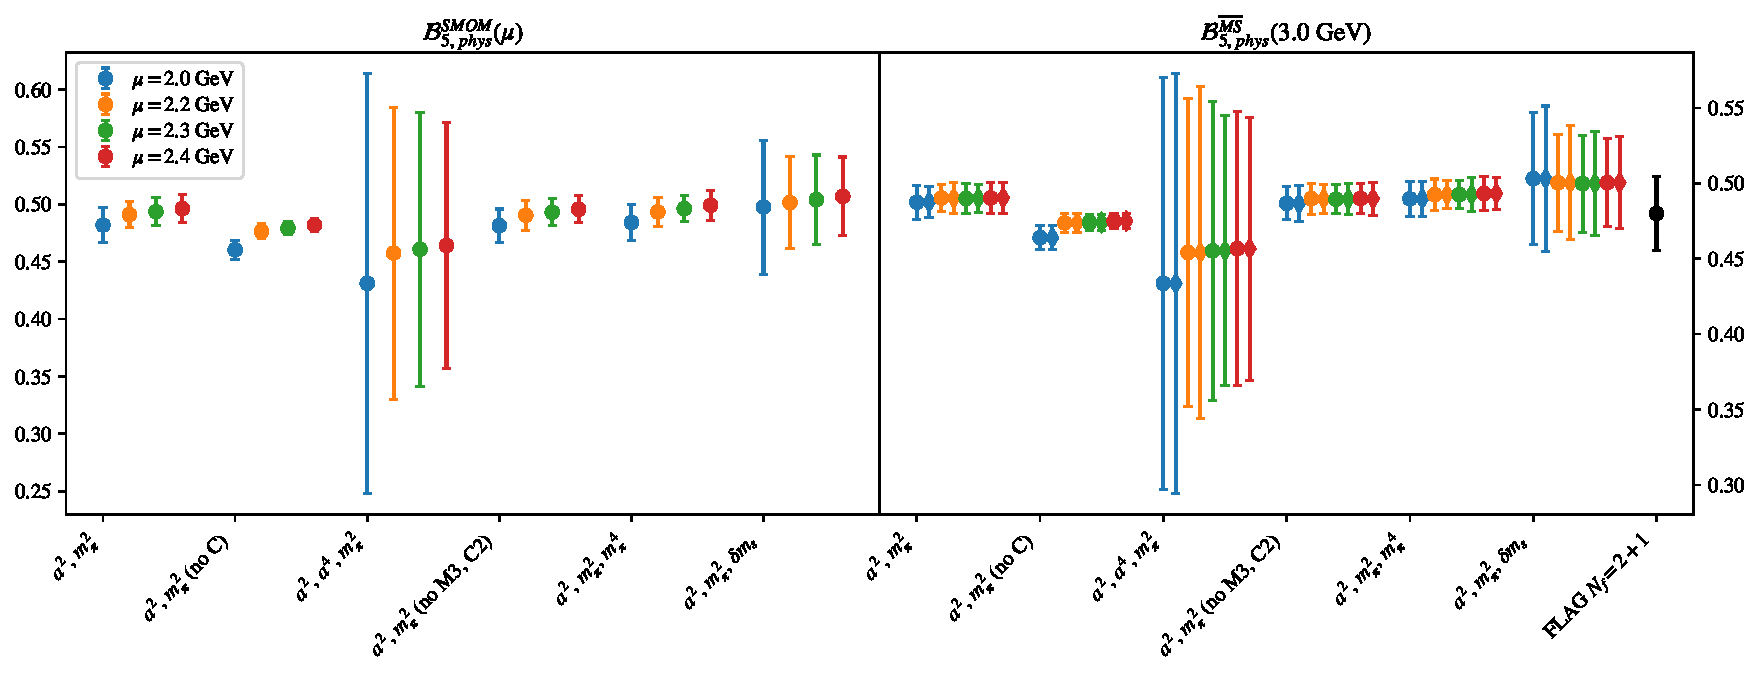
\includegraphics[page=1, width=1.1\textwidth]{TT/SUSY/fit_summary_bag.pdf}
\caption{$\mathcal{B}_{5}$\\(left) $\mathcal{B}_{phys}$ in RI/SMOM scheme from fit variations (fits with $p$-value $<0.05$ marked with ``$\times$"). \\(right) $\mathcal{B}_{phys}$ in $\overline{MS}$ computed using $\mathcal{B}^{\overline{MS}} = R^{\overline{MS}\leftarrow SMOM}(3.0)\sigma_{npt}(3.0,\mu) \mathcal{B}^{SMOM}(\mu)$.}
\end{figure}
\clearpage
\section{$\mathcal{B}_1$}
\begin{table}[h!]
\begin{center}
\begin{tabular}{|c|c|c|c|c|c|c|}
\hline
$\mu$ (GeV) & $a^2$, $m_\pi^2$& $a^2$, $m_\pi^2$ (no C)& $a^2$, $a^4$, $m_\pi^2$& $a^2$, $m_\pi^2$ (no M3, C2)& $a^2$, $m_\pi^2$, $m_\pi^4$& $a^2$, $m_\pi^2$, $\delta m_s$\\
\hline
2.0& \hyperlink{VVpAA/SUSY/a2m2_20.pdf.1}{\textbf{1.4038(27)}: 1.86 (0.098)} & \hyperlink{VVpAA/SUSY/a2m2noC_20.pdf.1}{\textbf{1.416(12)}: 0.917 (0.4)} & \hyperlink{VVpAA/SUSY/a2a4m2_20.pdf.1}{\textbf{1.421(21)}: 2.155 (0.071)} & \hyperlink{VVpAA/SUSY/a2m2mcut_20.pdf.1}{\textbf{1.4089(32)}: 0.264 (0.851)} & \hyperlink{VVpAA/SUSY/a2m2m4_20.pdf.1}{\textbf{1.4092(33)}: 0.695 (0.595)} & \hyperlink{VVpAA/SUSY/a2m2delm_20.pdf.1}{\textbf{1.4016(32)}: 1.869 (0.113)}\\
2.2& \hyperlink{VVpAA/SUSY/a2m2_22.pdf.1}{\textbf{1.3963(27)}: 2.192 (0.052)} & \hyperlink{VVpAA/SUSY/a2m2noC_22.pdf.1}{\textbf{1.410(12)}: 1.158 (0.314)} & \hyperlink{VVpAA/SUSY/a2a4m2_22.pdf.1}{\textbf{1.417(21)}: 2.498 (0.041)} & \hyperlink{VVpAA/SUSY/a2m2mcut_22.pdf.1}{\textbf{1.4018(32)}: 0.361 (0.781)} & \hyperlink{VVpAA/SUSY/a2m2m4_22.pdf.1}{\textbf{1.4020(33)}: 0.916 (0.453)} & \hyperlink{VVpAA/SUSY/a2m2delm_22.pdf.1}{\textbf{1.3937(32)}: 2.121 (0.075)}\\
2.3& \hyperlink{VVpAA/SUSY/a2m2_23.pdf.1}{\textbf{1.3931(26)}: 2.28 (0.044)} & \hyperlink{VVpAA/SUSY/a2m2noC_23.pdf.1}{\textbf{1.408(12)}: 1.204 (0.3)} & \hyperlink{VVpAA/SUSY/a2a4m2_23.pdf.1}{\textbf{1.415(21)}: 2.575 (0.036)} & \hyperlink{VVpAA/SUSY/a2m2mcut_23.pdf.1}{\textbf{1.3986(32)}: 0.411 (0.745)} & \hyperlink{VVpAA/SUSY/a2m2m4_23.pdf.1}{\textbf{1.3988(33)}: 0.984 (0.415)} & \hyperlink{VVpAA/SUSY/a2m2delm_23.pdf.1}{\textbf{1.3903(32)}: 2.164 (0.07)}\\
2.4& \hyperlink{VVpAA/SUSY/a2m2_24.pdf.1}{\textbf{1.3902(26)}: 2.328 (0.04)} & \hyperlink{VVpAA/SUSY/a2m2noC_24.pdf.1}{\textbf{1.405(12)}: 1.229 (0.293)} & \hyperlink{VVpAA/SUSY/a2a4m2_24.pdf.1}{\textbf{1.412(21)}: 2.636 (0.032)} & \hyperlink{VVpAA/SUSY/a2m2mcut_24.pdf.1}{\textbf{1.3958(32)}: 0.413 (0.744)} & \hyperlink{VVpAA/SUSY/a2m2m4_24.pdf.1}{\textbf{1.3960(33)}: 1.0 (0.406)} & \hyperlink{VVpAA/SUSY/a2m2delm_24.pdf.1}{\textbf{1.3874(32)}: 2.211 (0.065)}\\
\hline
\end{tabular}
\caption{Physical point value from chiral and continuum extrapolation at renormalisation scale $\mu$. Entries are \textbf{value(error)}: $\chi^2/\text{DOF}$ ($p$-value).}
\end{center}
\end{table}
\begin{table}[h!]
\begin{center}
\begin{tabular}{|c c|c|c|c|c|c|c|}
\hline
$\mu$ (GeV) &  & $a^2$, $m_\pi^2$& $a^2$, $m_\pi^2$ (no C)& $a^2$, $a^4$, $m_\pi^2$& $a^2$, $m_\pi^2$ (no M3, C2)& $a^2$, $m_\pi^2$, $m_\pi^4$& $a^2$, $m_\pi^2$, $\delta m_s$\\
\hline
\multirow{2}{0.5in}{2.0} & $\alpha$ & 0.0936(70)& 0.047(52)& -0.021& 0.0814(83)& 0.0812(83)& 0.0987(81)\\
 & $\beta$ & 0.00261(14)& 0.00224(27)& 0.00263(14)& 0.00189(28)& 0.00033(89)& 0.00269(15)\\
\hline
\multirow{2}{0.5in}{2.2} & $\alpha$ & 0.0978(70)& 0.042(52)& -0.039& 0.0848(84)& 0.0847(83)& 0.1039(81)\\
 & $\beta$ & 0.00261(14)& 0.00221(27)& 0.00264(14)& 0.00183(28)& 0.00020(89)& 0.00271(16)\\
\hline
\multirow{2}{0.5in}{2.3} & $\alpha$ & 0.0993(70)& 0.039(52)& -0.046& 0.0860(84)& 0.0860(83)& 0.1057(81)\\
 & $\beta$ & 0.00262(14)& 0.00221(27)& 0.00265(14)& 0.00183(28)& 0.00019(89)& 0.00272(16)\\
\hline
\multirow{2}{0.5in}{2.4} & $\alpha$ & 0.1000(70)& 0.040(52)& -0.045& 0.0865(84)& 0.0865(83)& 0.1064(81)\\
 & $\beta$ & 0.00263(14)& 0.00221(27)& 0.00267(14)& 0.00184(28)& 0.00017(89)& 0.00273(16)\\
\hline
\end{tabular}
\caption{Fit values of coefficients in $Q = Q_{phys} + \mathbf{\alpha} a^2 + \mathbf{\beta}\left(\frac{m_\pi^2}{f_\pi^2}-\frac{m_{\pi,PDG}^2}{f_\pi^2}\right) + \ldots$.}
\end{center}
\end{table}
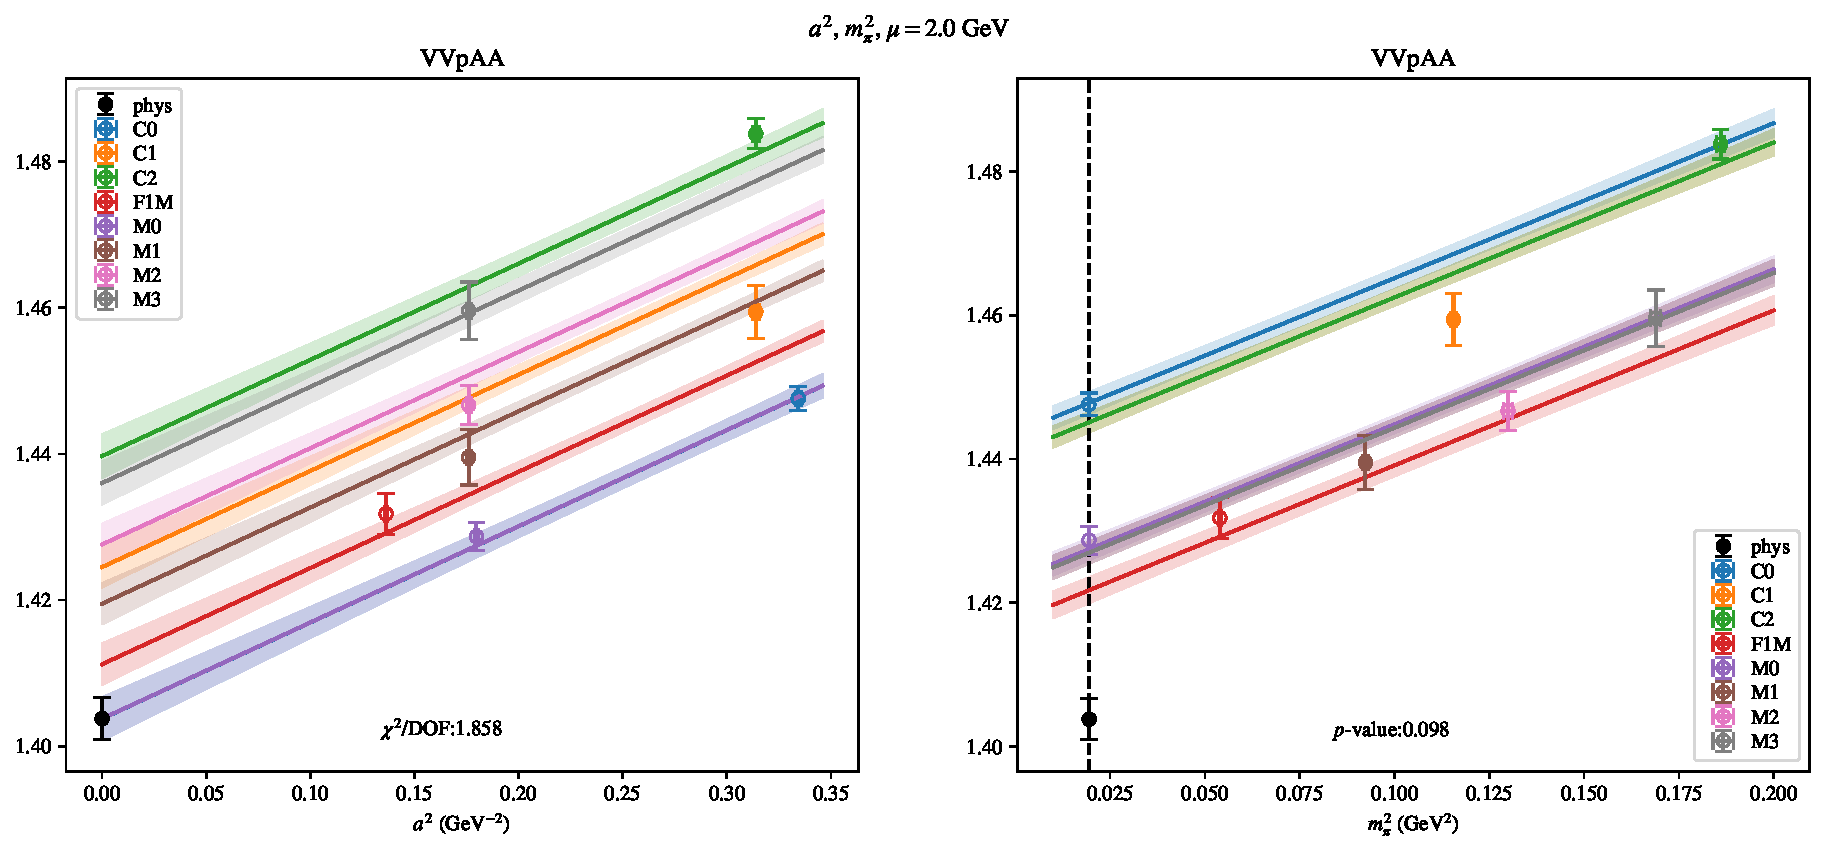
\includepdf[link, pages=-]{VVpAA/SUSY/a2m2_20.pdf}
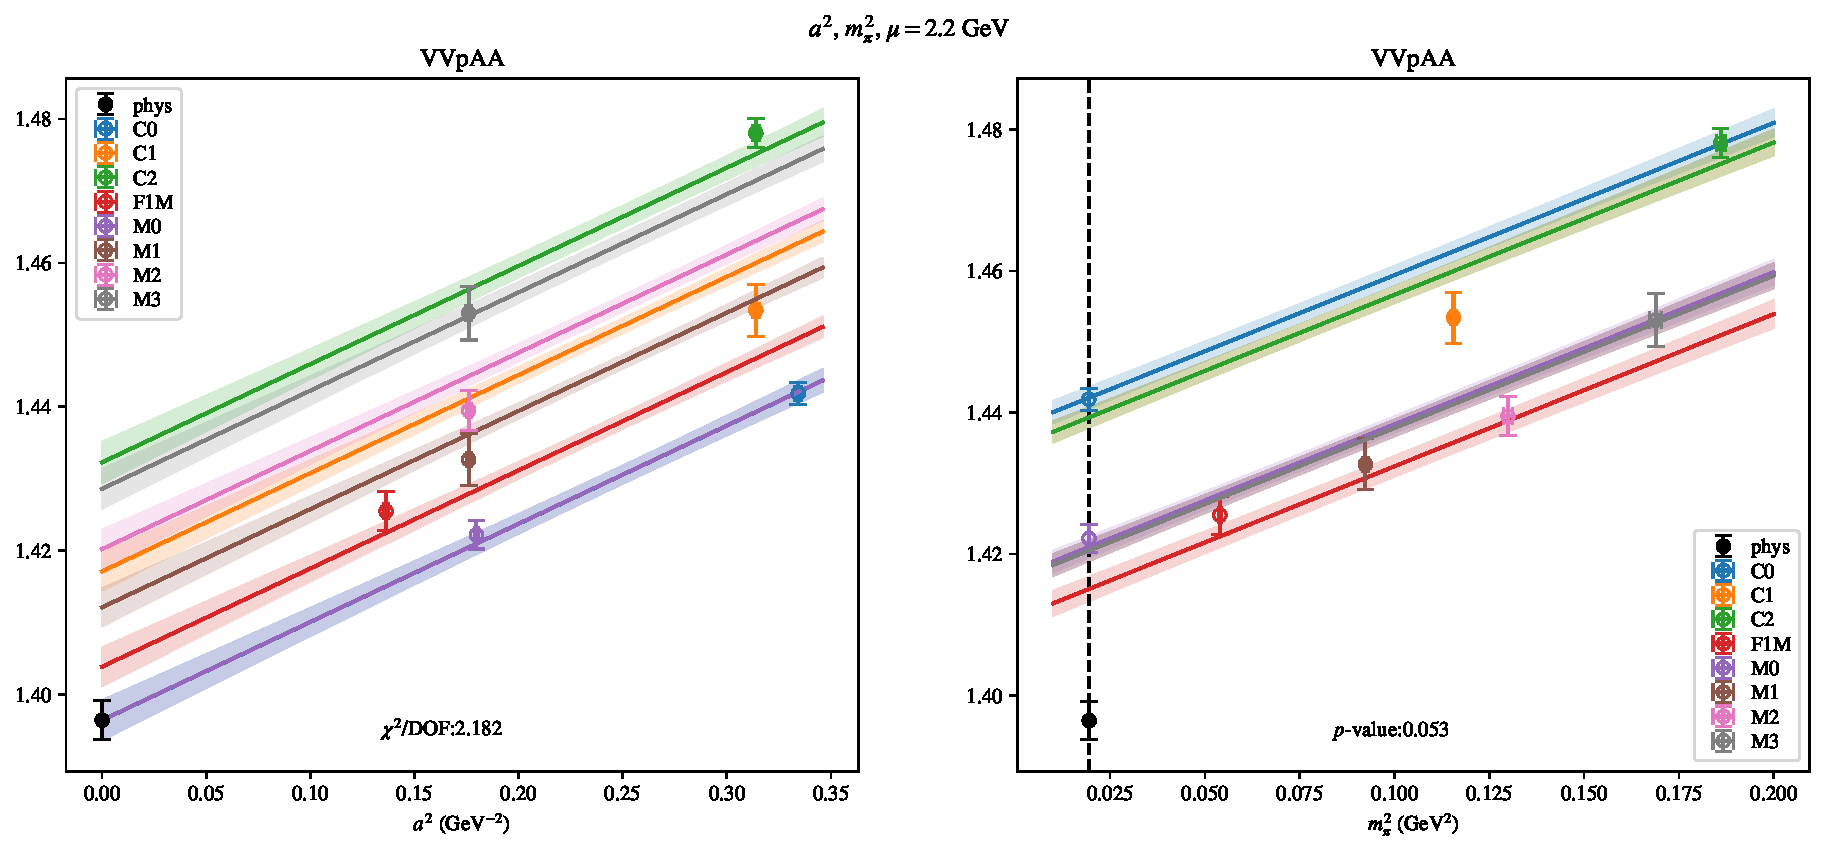
\includepdf[link, pages=-]{VVpAA/SUSY/a2m2_22.pdf}
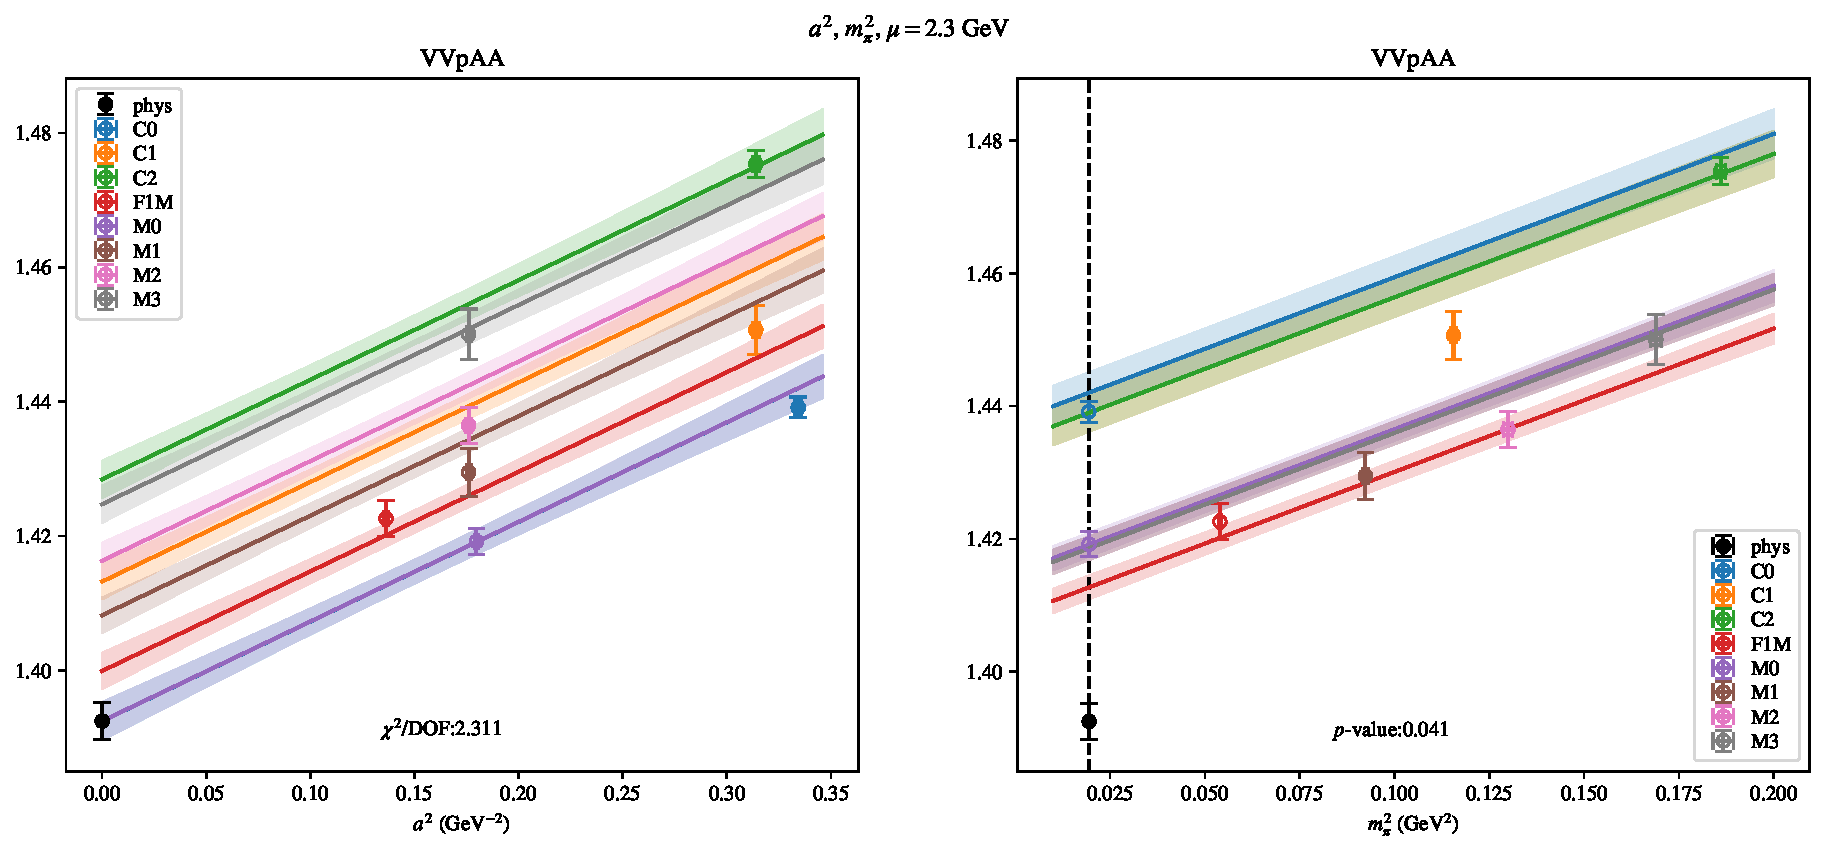
\includepdf[link, pages=-]{VVpAA/SUSY/a2m2_23.pdf}
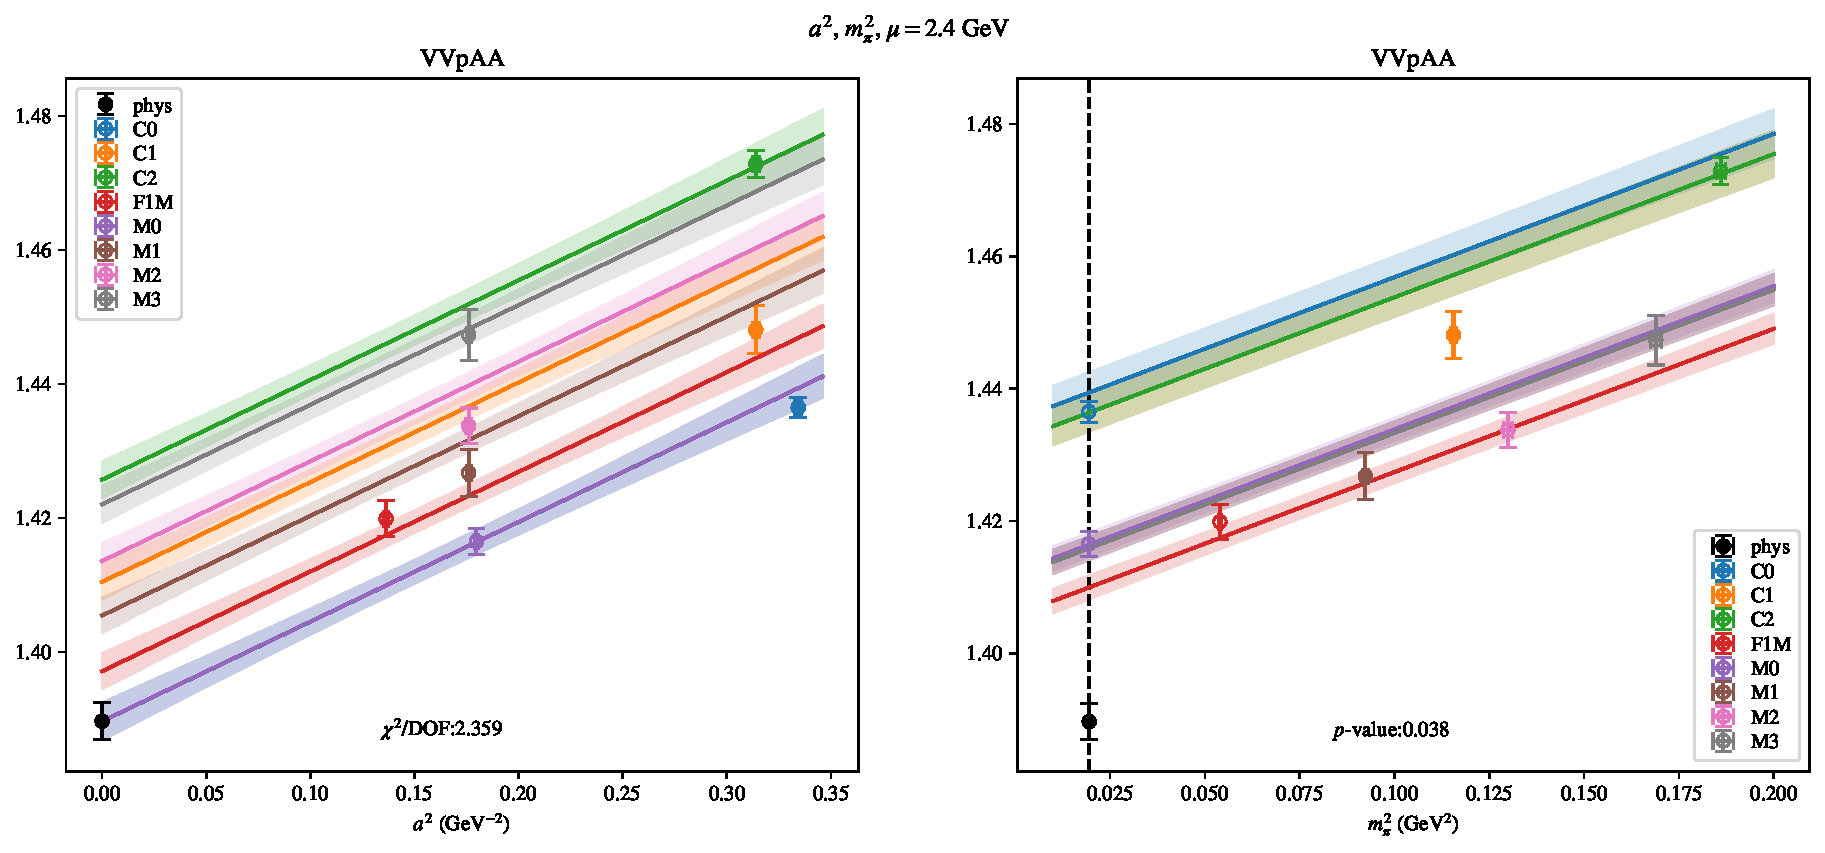
\includepdf[link, pages=-]{VVpAA/SUSY/a2m2_24.pdf}
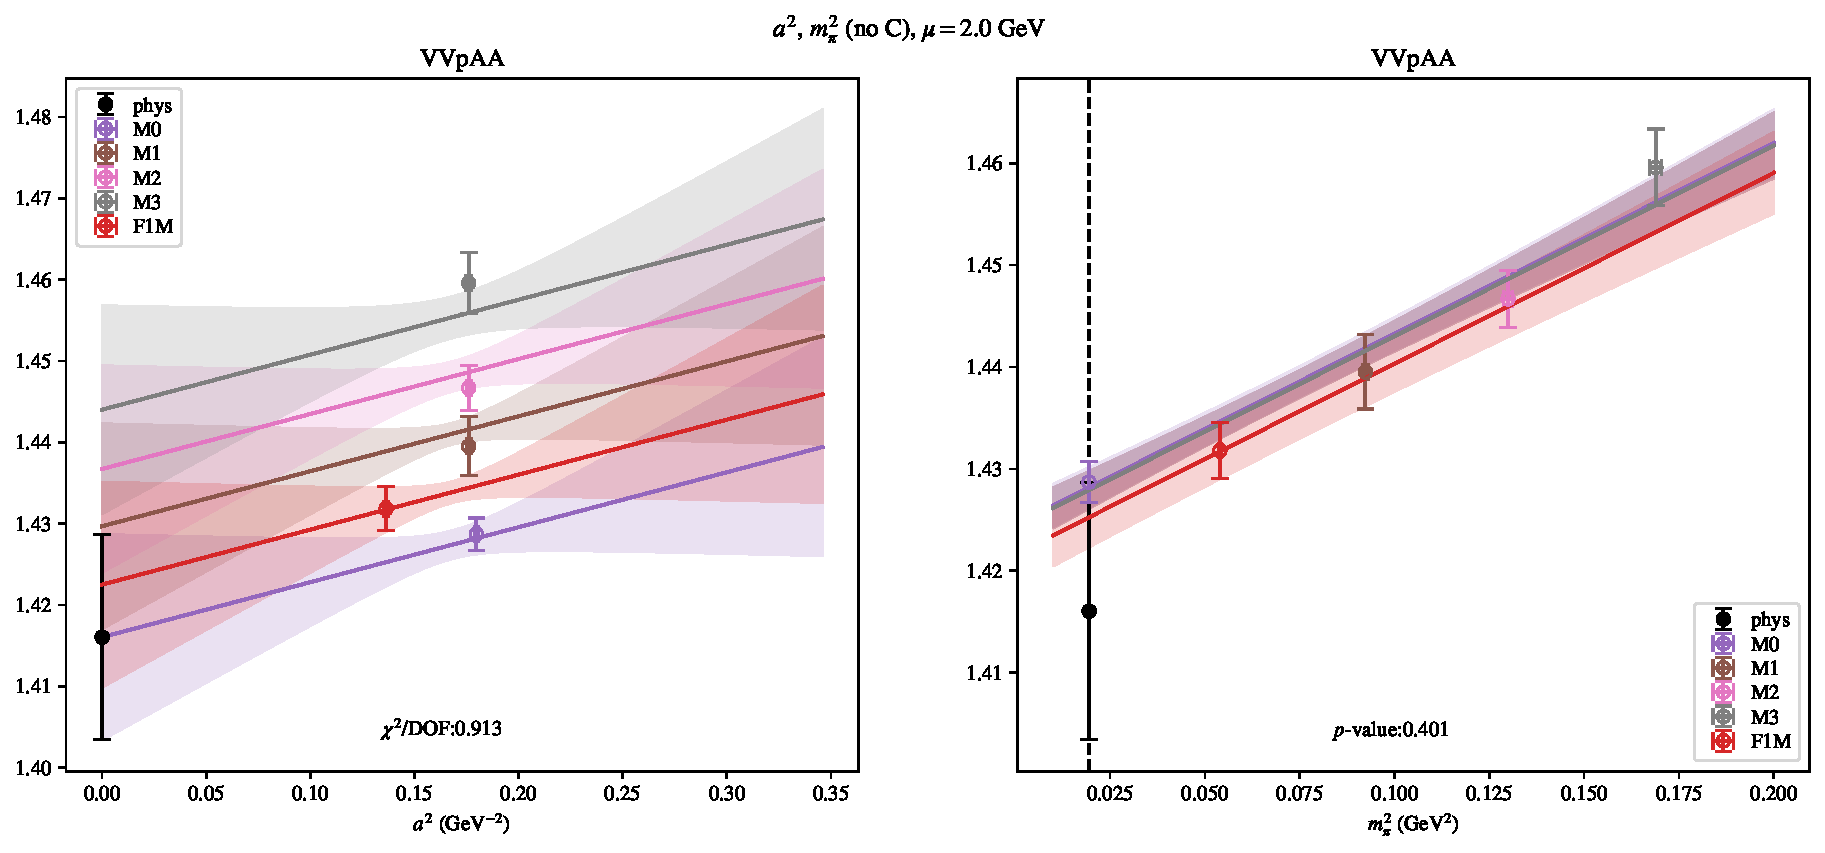
\includepdf[link, pages=-]{VVpAA/SUSY/a2m2noC_20.pdf}
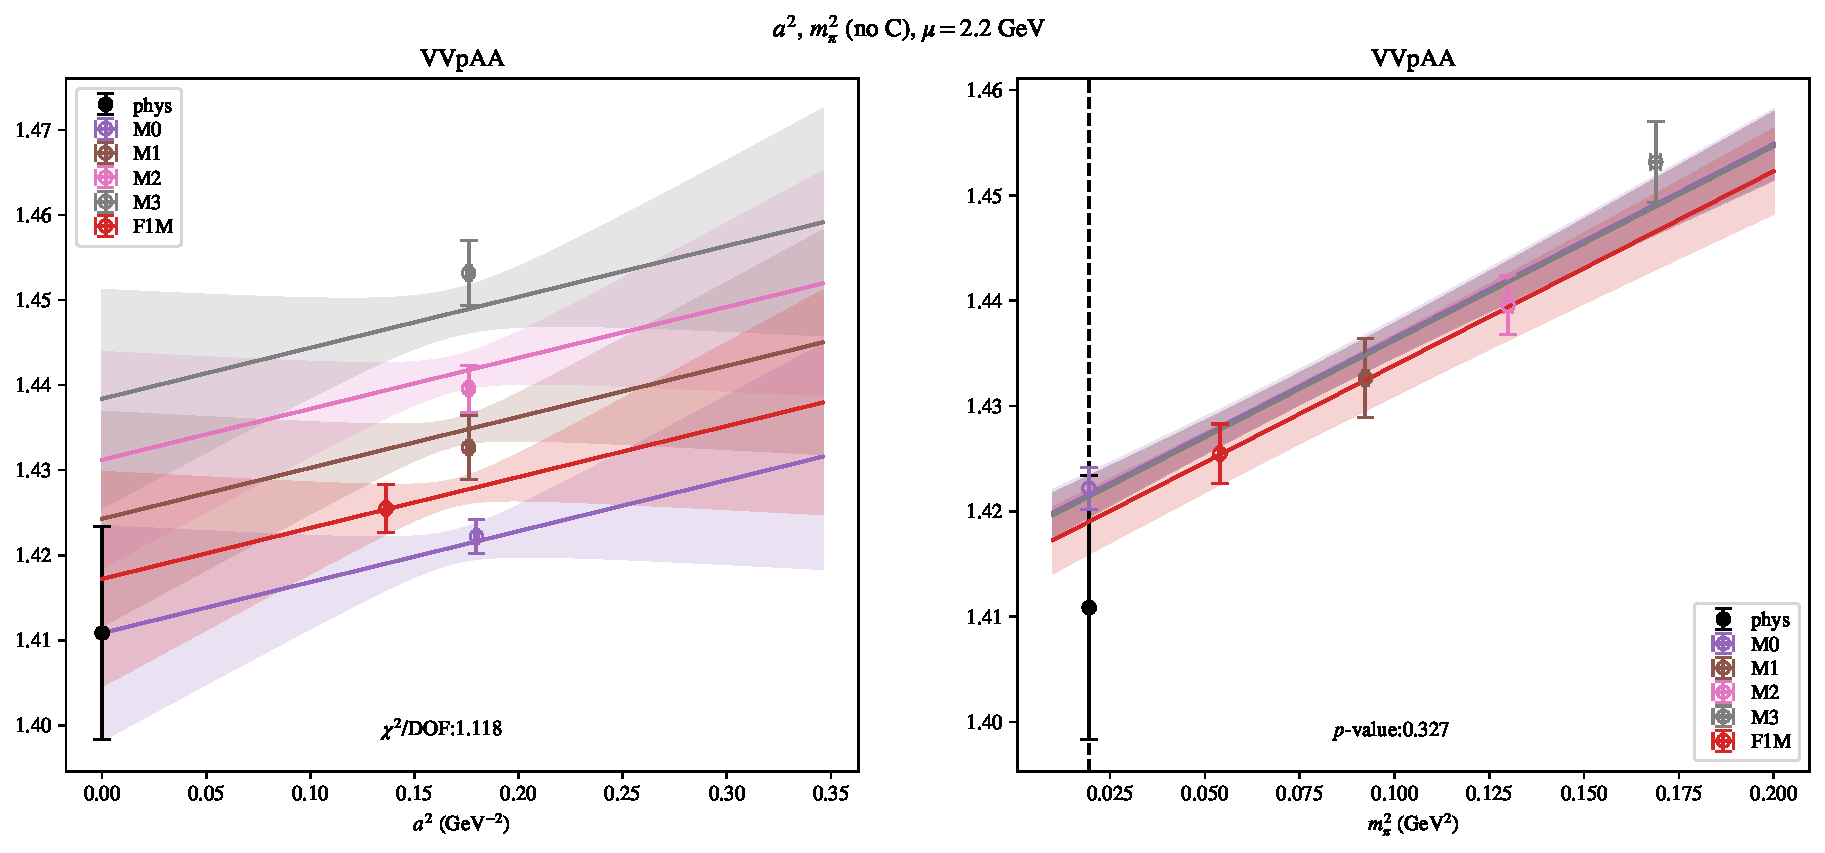
\includepdf[link, pages=-]{VVpAA/SUSY/a2m2noC_22.pdf}
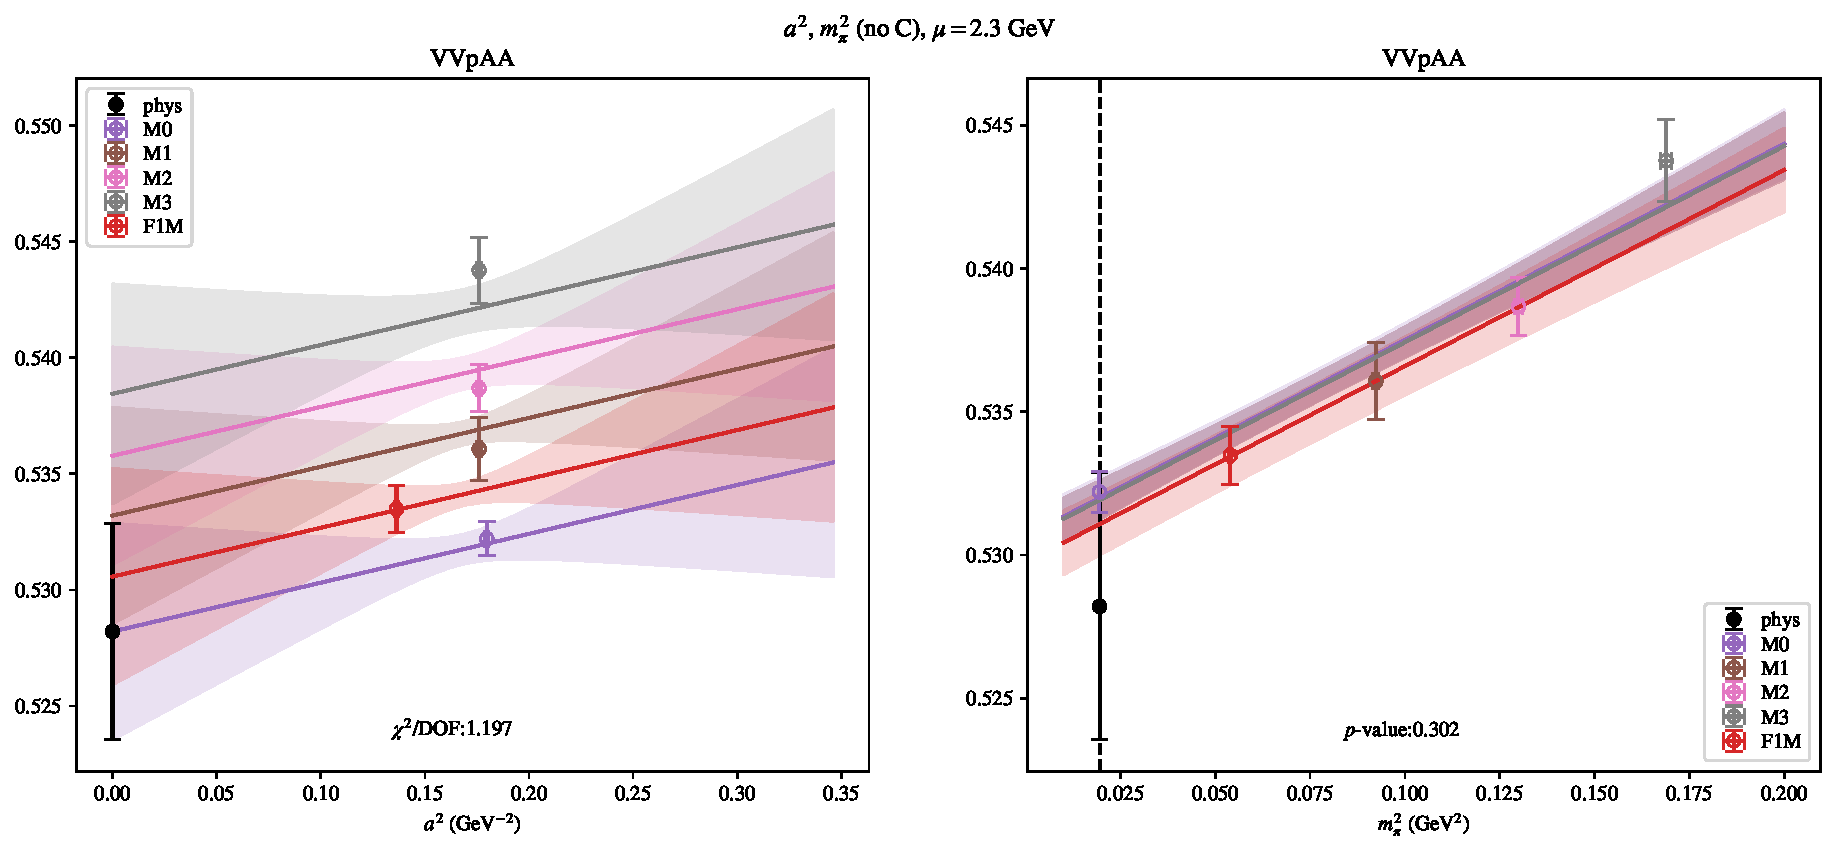
\includepdf[link, pages=-]{VVpAA/SUSY/a2m2noC_23.pdf}
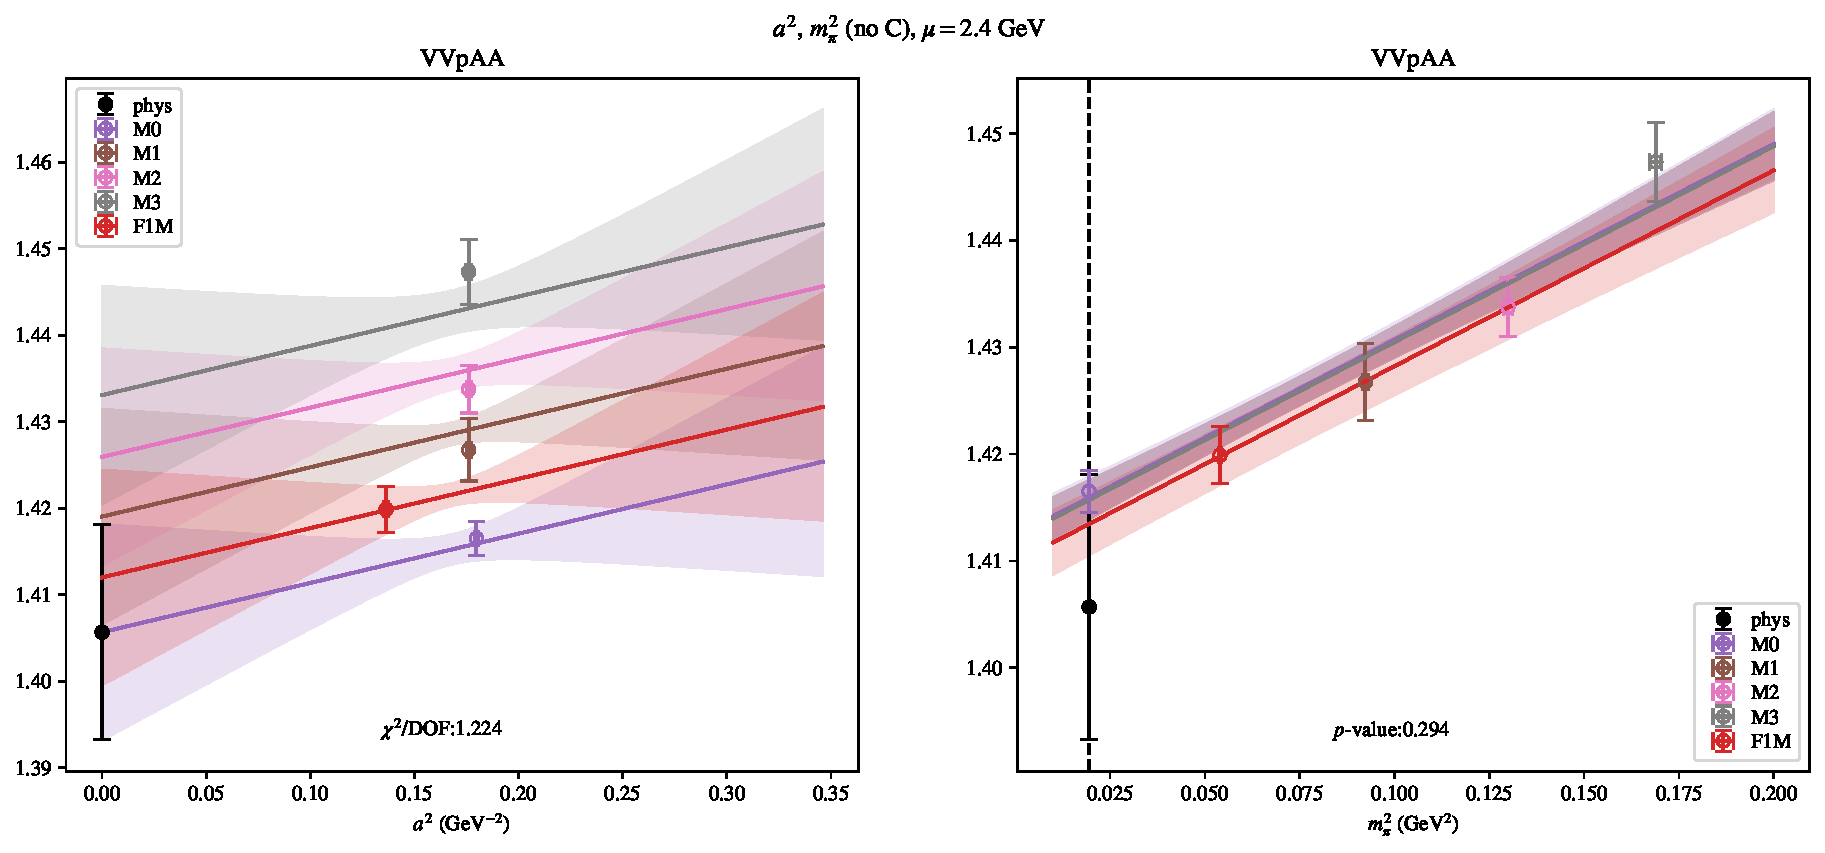
\includepdf[link, pages=-]{VVpAA/SUSY/a2m2noC_24.pdf}
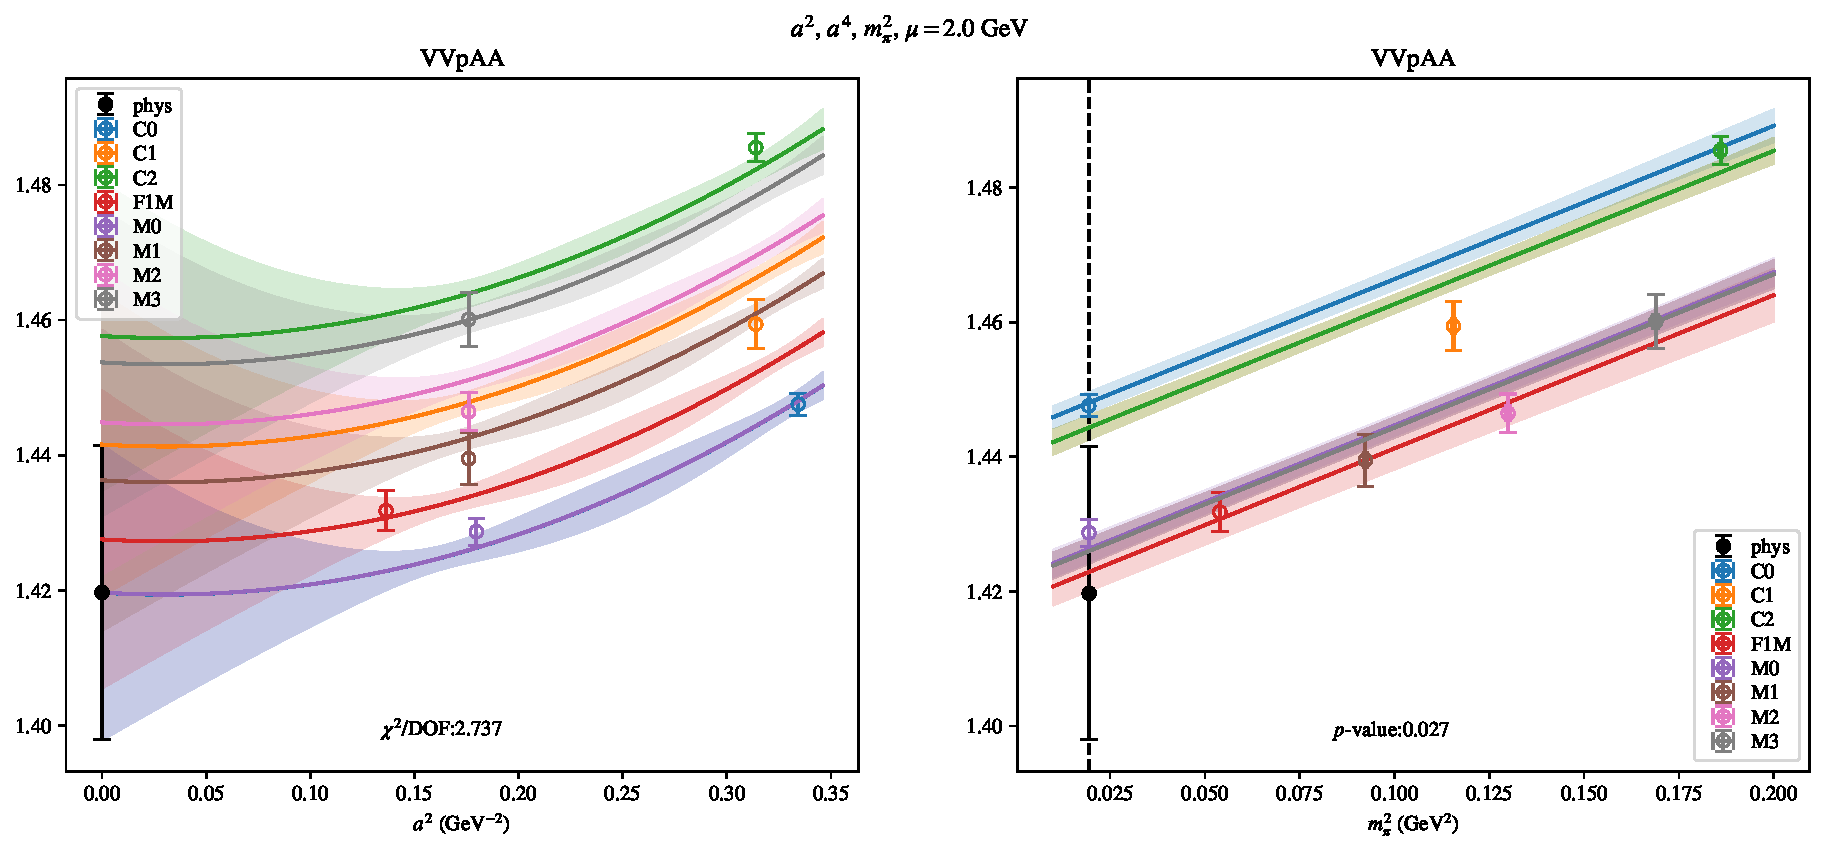
\includepdf[link, pages=-]{VVpAA/SUSY/a2a4m2_20.pdf}
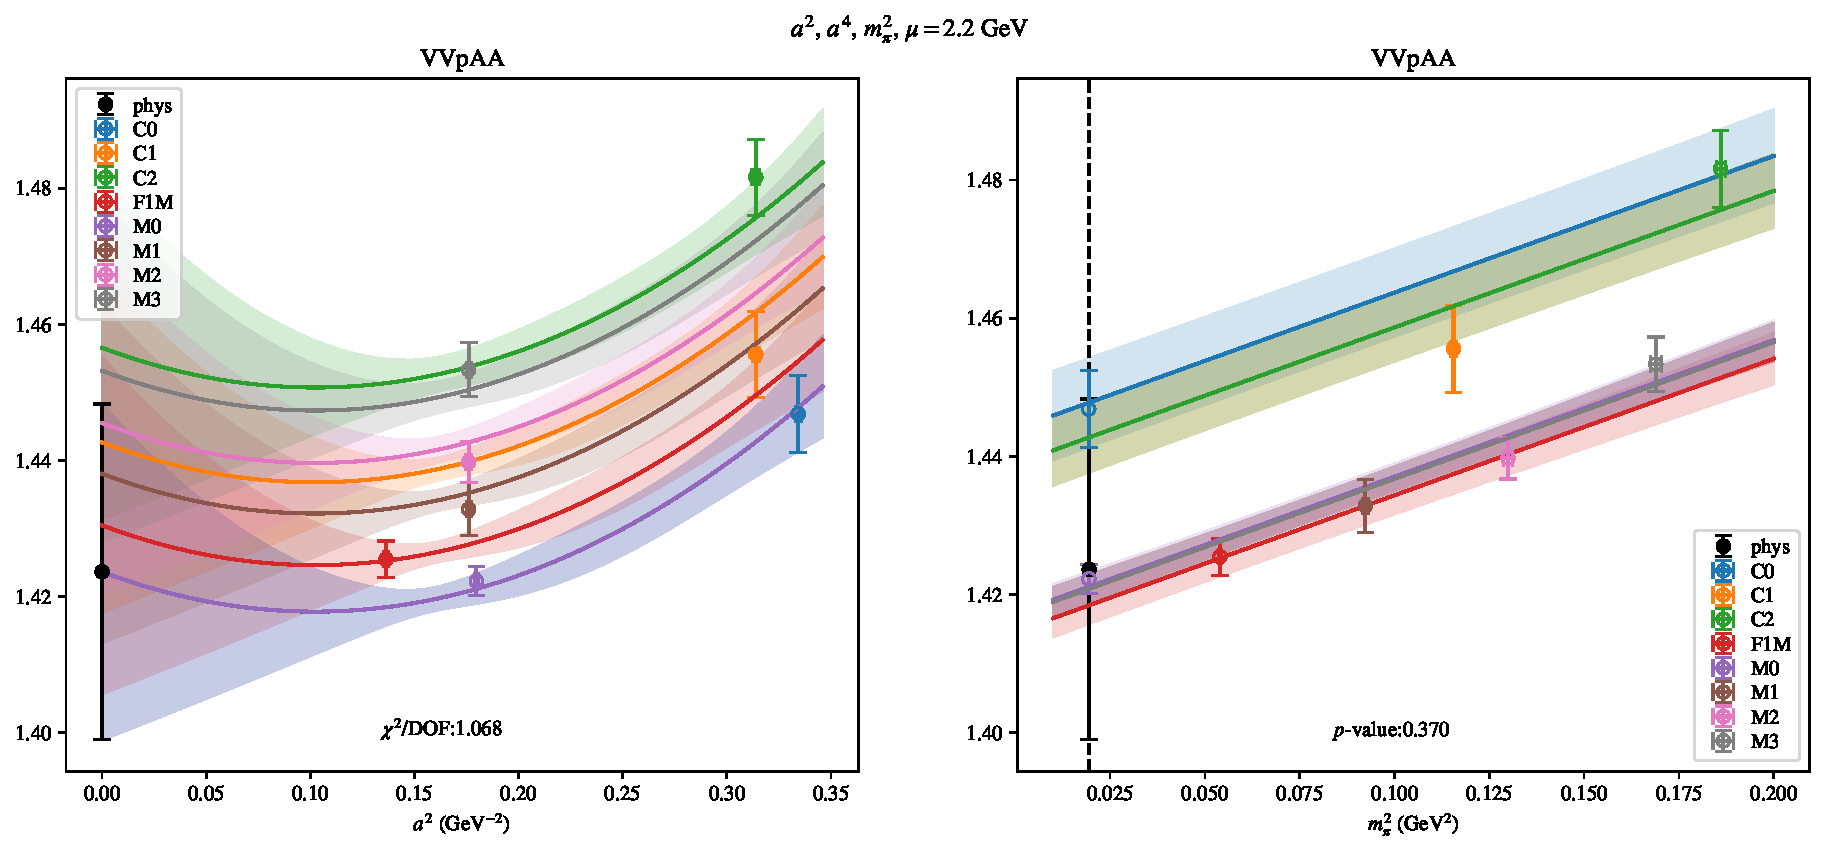
\includepdf[link, pages=-]{VVpAA/SUSY/a2a4m2_22.pdf}
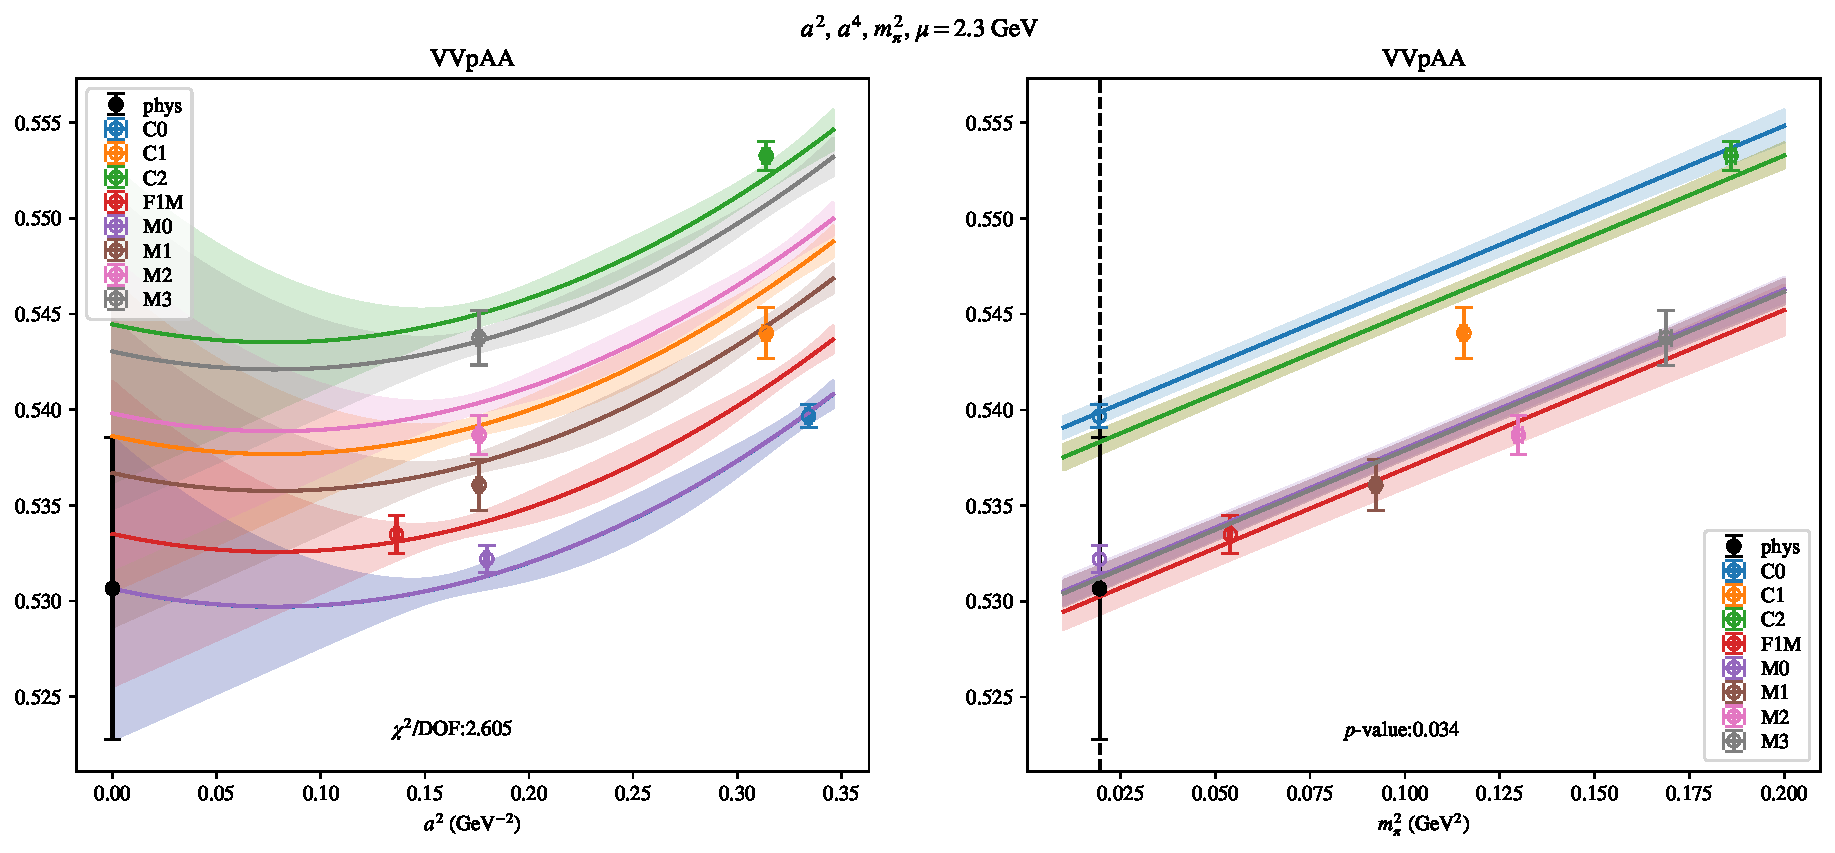
\includepdf[link, pages=-]{VVpAA/SUSY/a2a4m2_23.pdf}
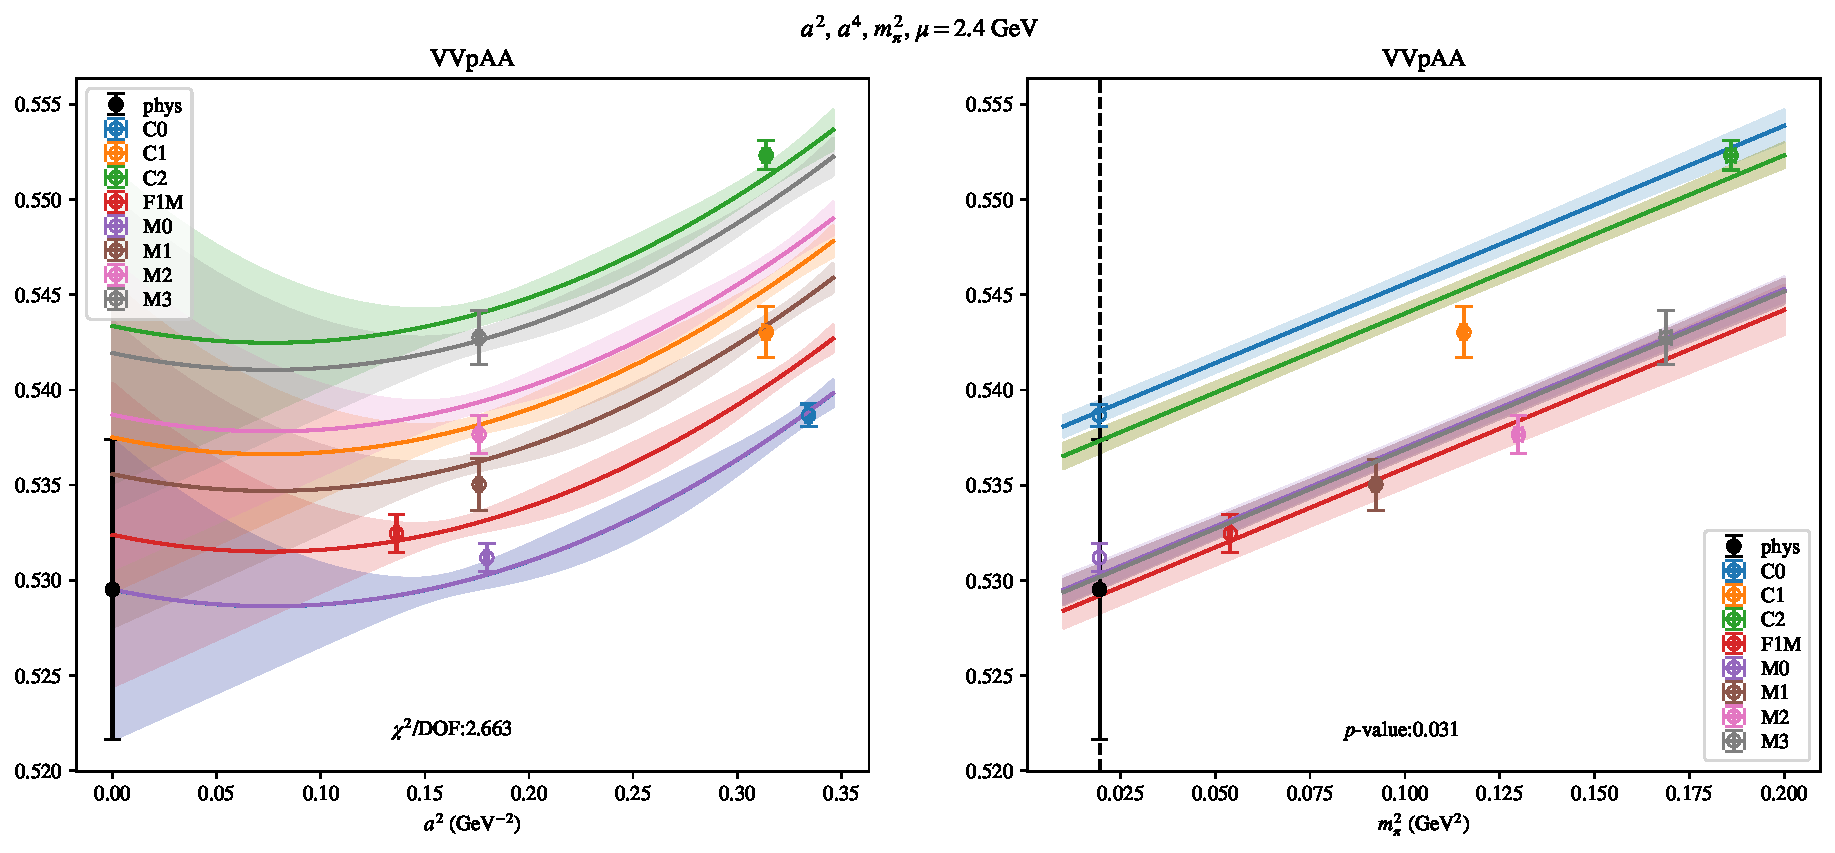
\includepdf[link, pages=-]{VVpAA/SUSY/a2a4m2_24.pdf}
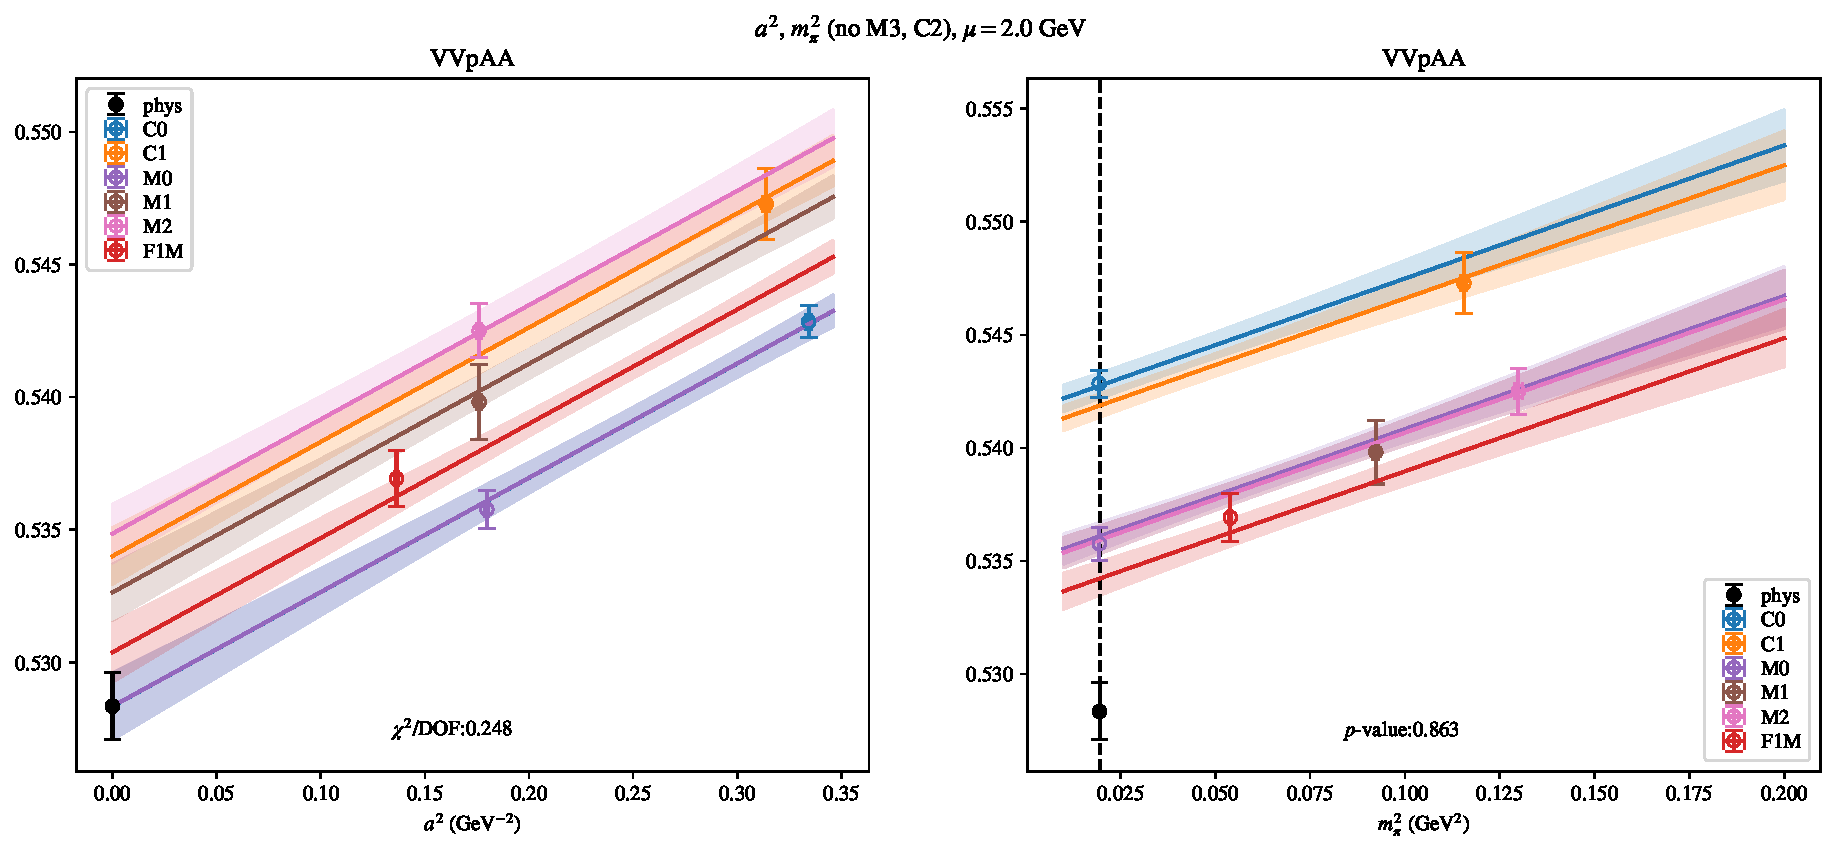
\includepdf[link, pages=-]{VVpAA/SUSY/a2m2mcut_20.pdf}
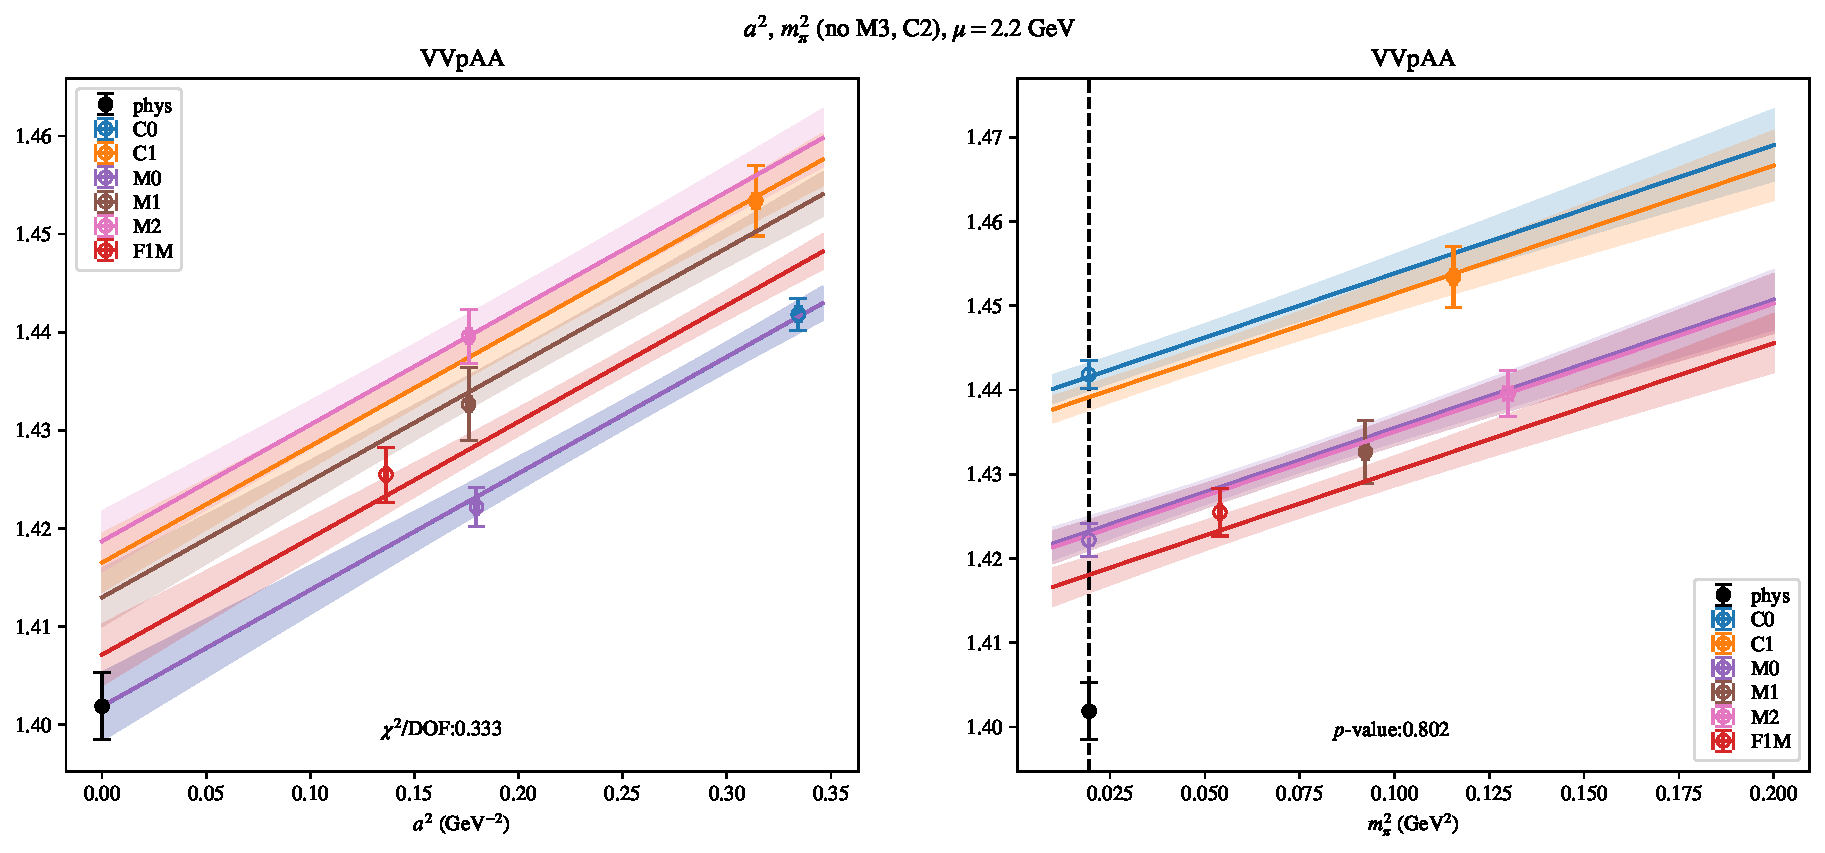
\includepdf[link, pages=-]{VVpAA/SUSY/a2m2mcut_22.pdf}
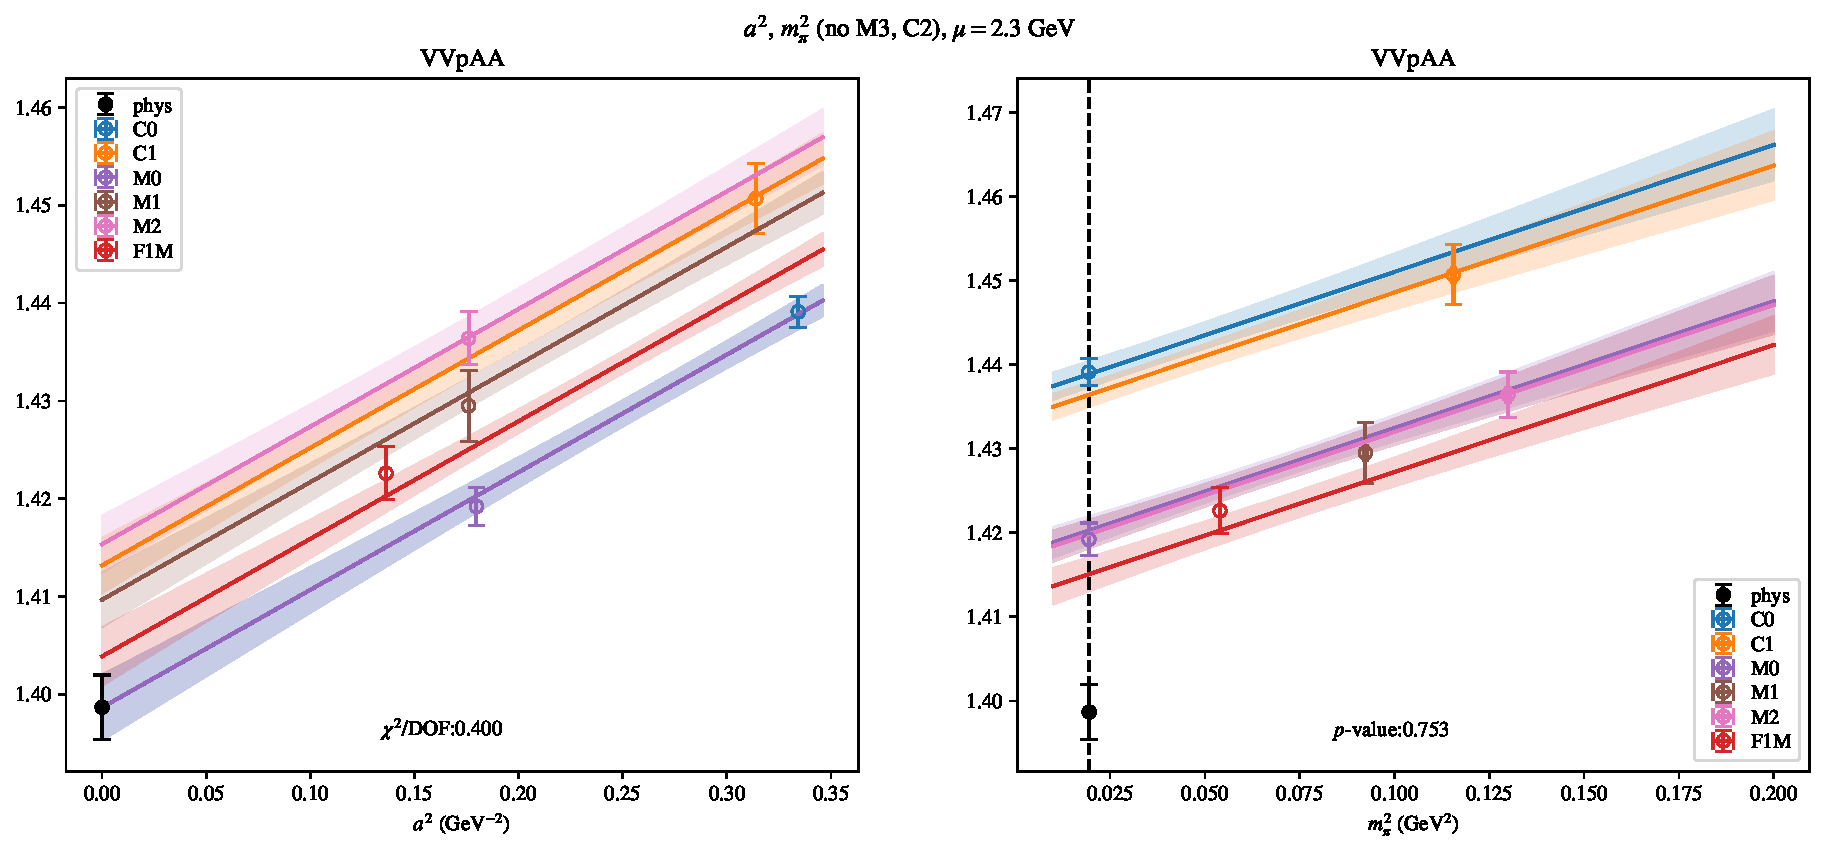
\includepdf[link, pages=-]{VVpAA/SUSY/a2m2mcut_23.pdf}
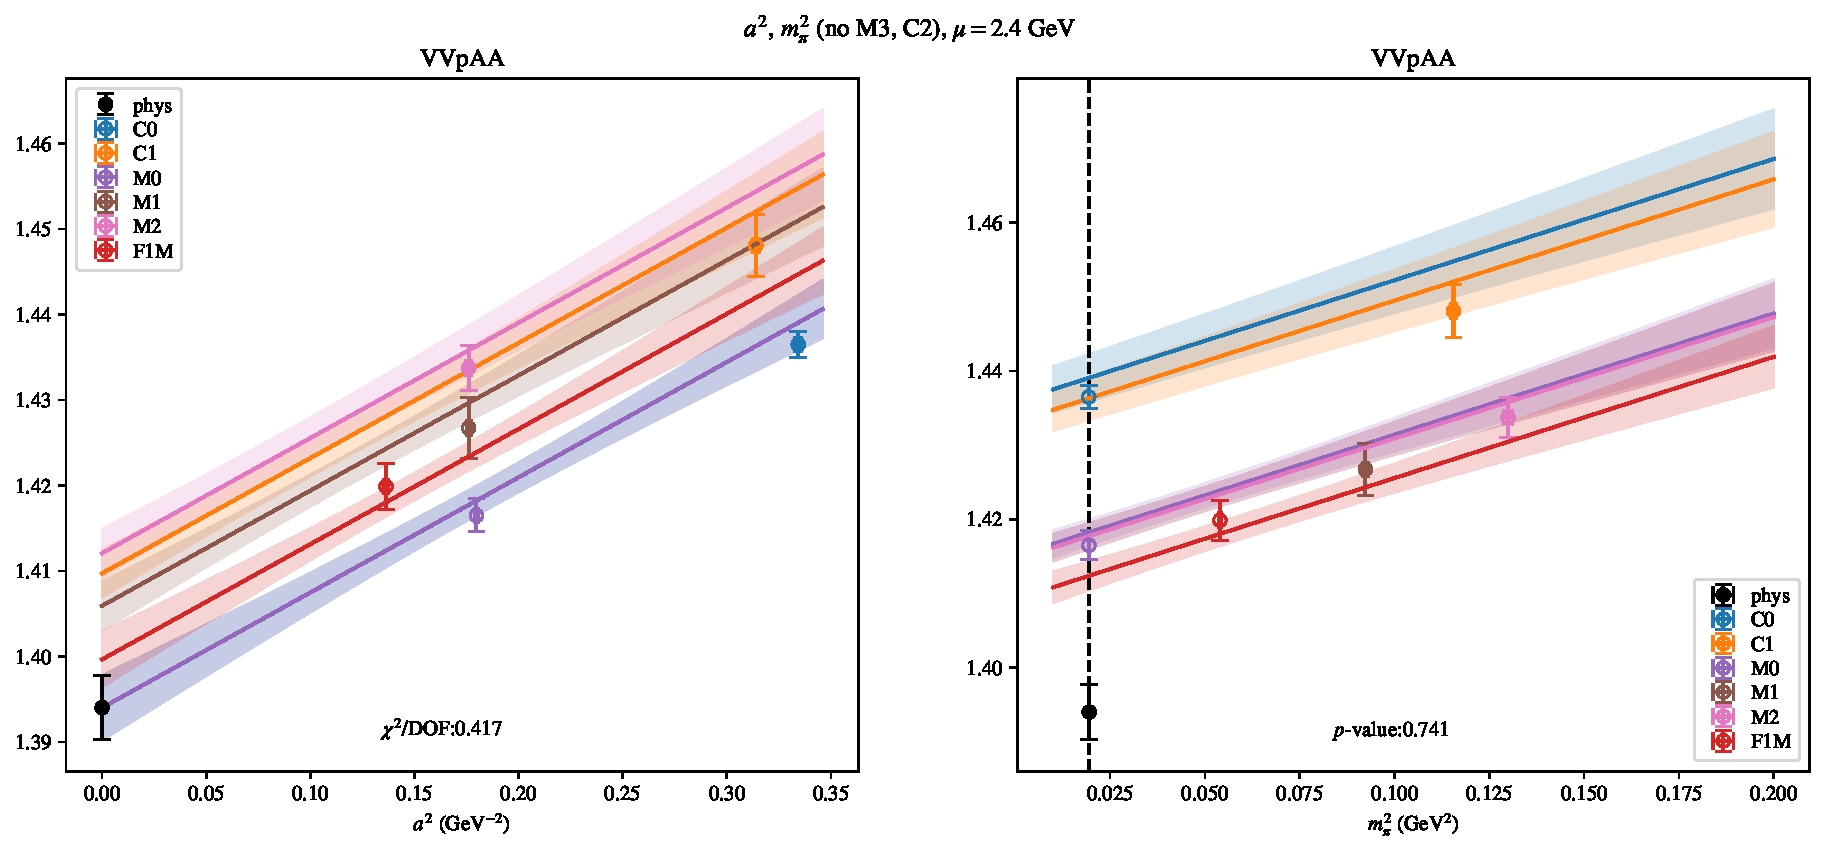
\includepdf[link, pages=-]{VVpAA/SUSY/a2m2mcut_24.pdf}
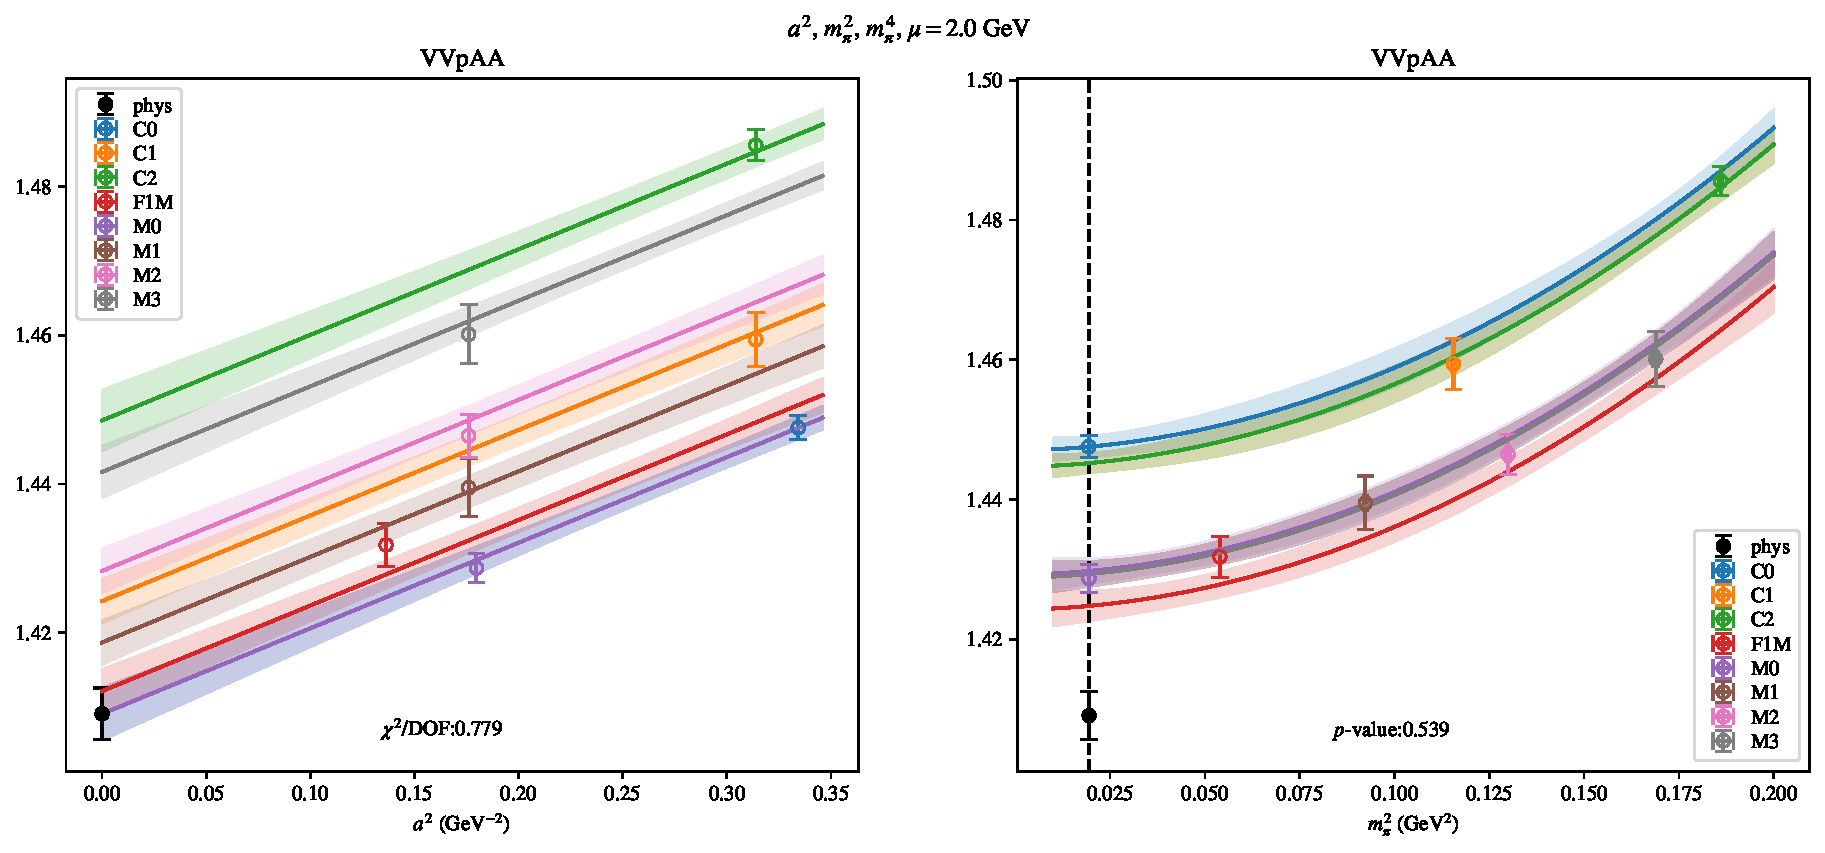
\includepdf[link, pages=-]{VVpAA/SUSY/a2m2m4_20.pdf}
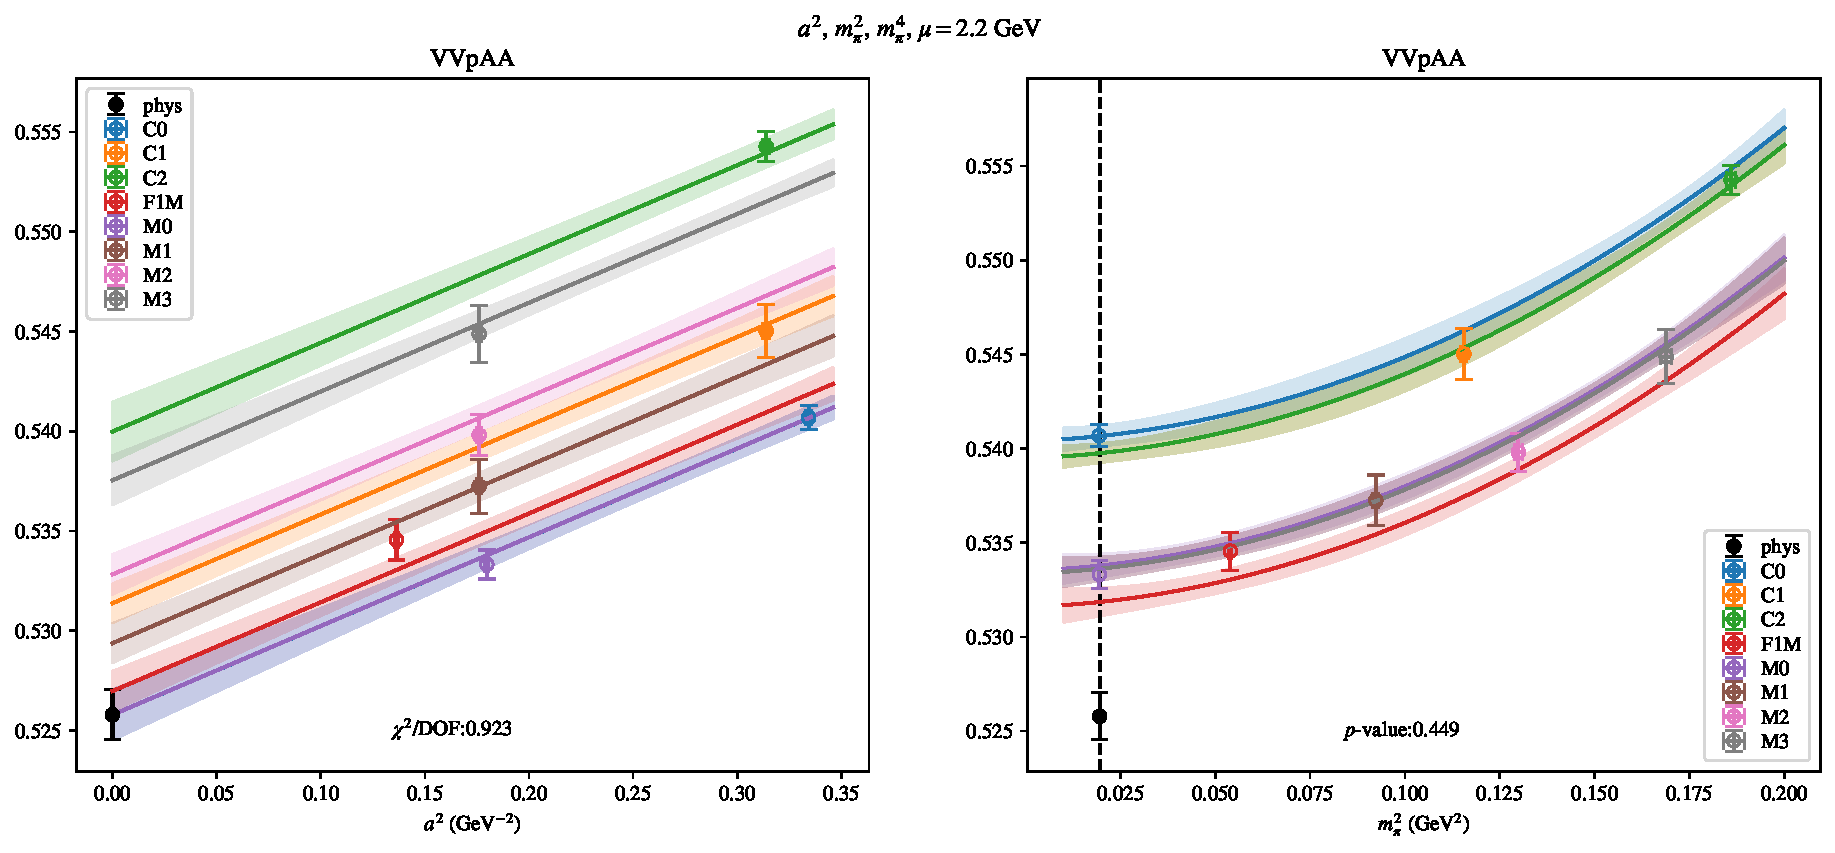
\includepdf[link, pages=-]{VVpAA/SUSY/a2m2m4_22.pdf}
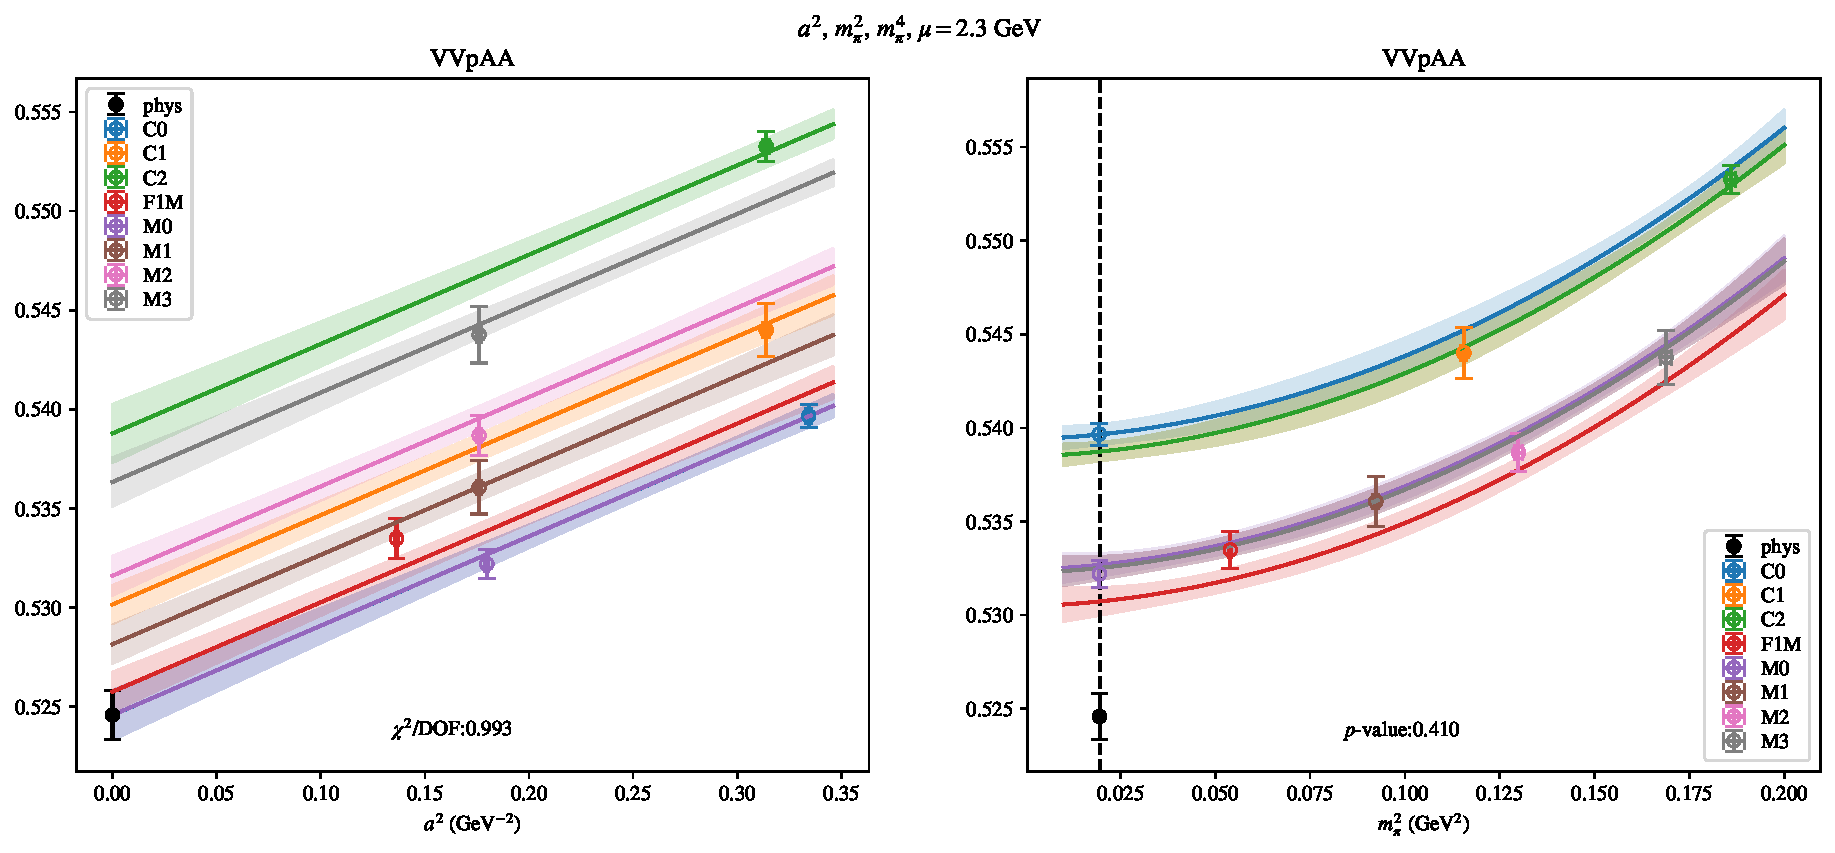
\includepdf[link, pages=-]{VVpAA/SUSY/a2m2m4_23.pdf}
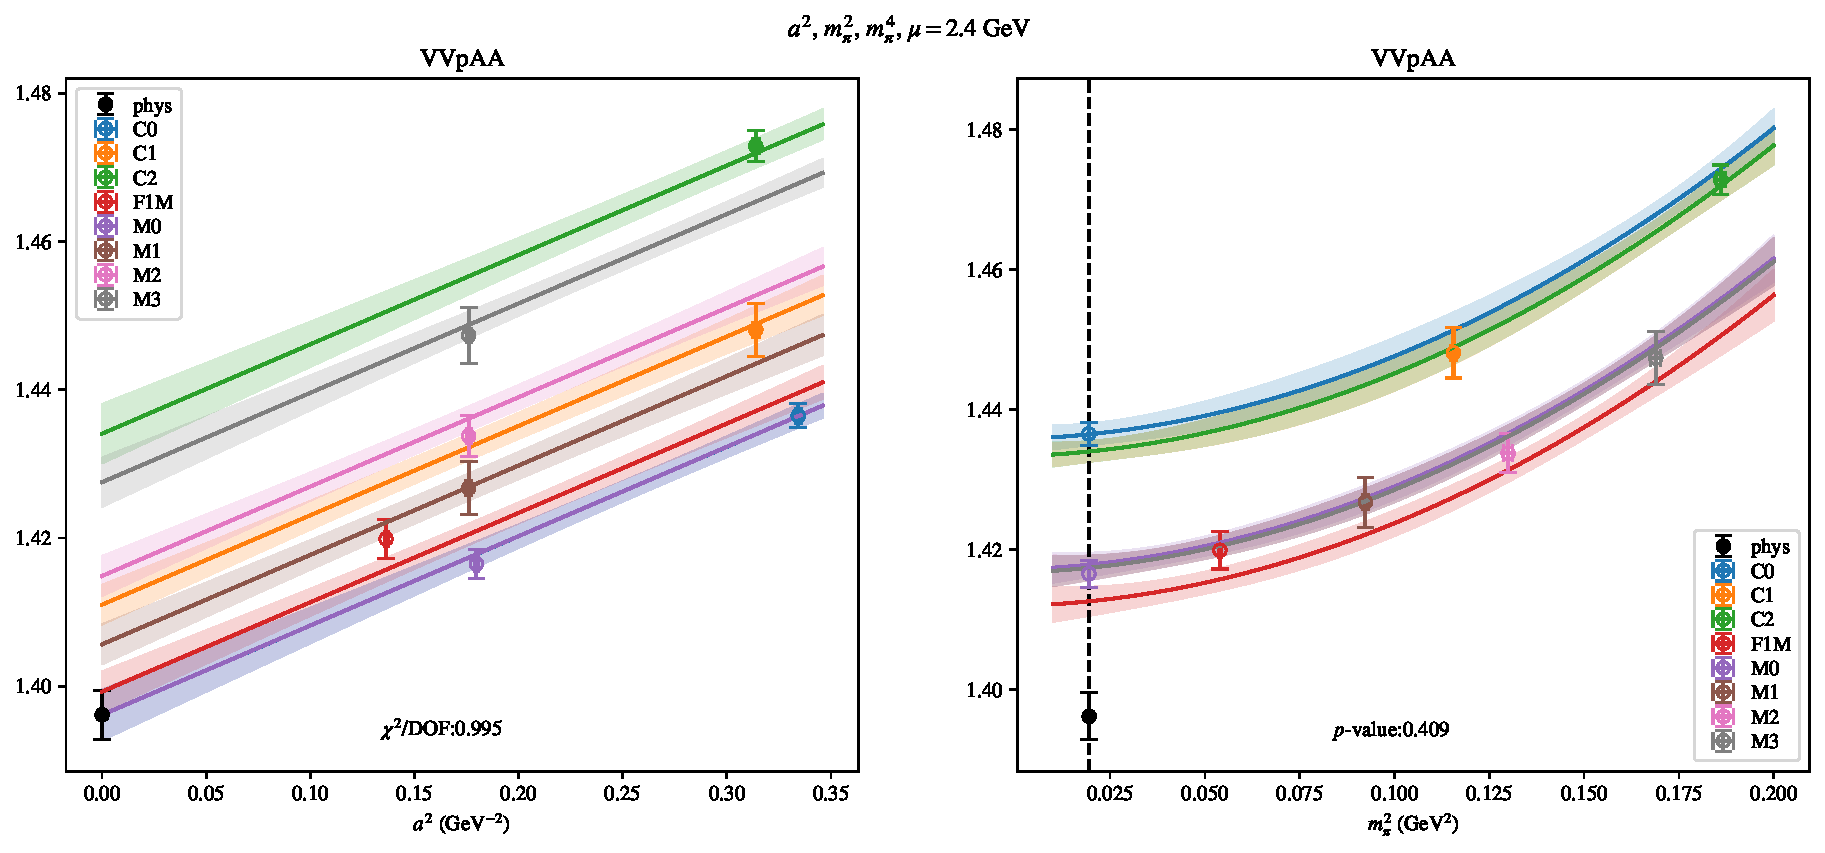
\includepdf[link, pages=-]{VVpAA/SUSY/a2m2m4_24.pdf}
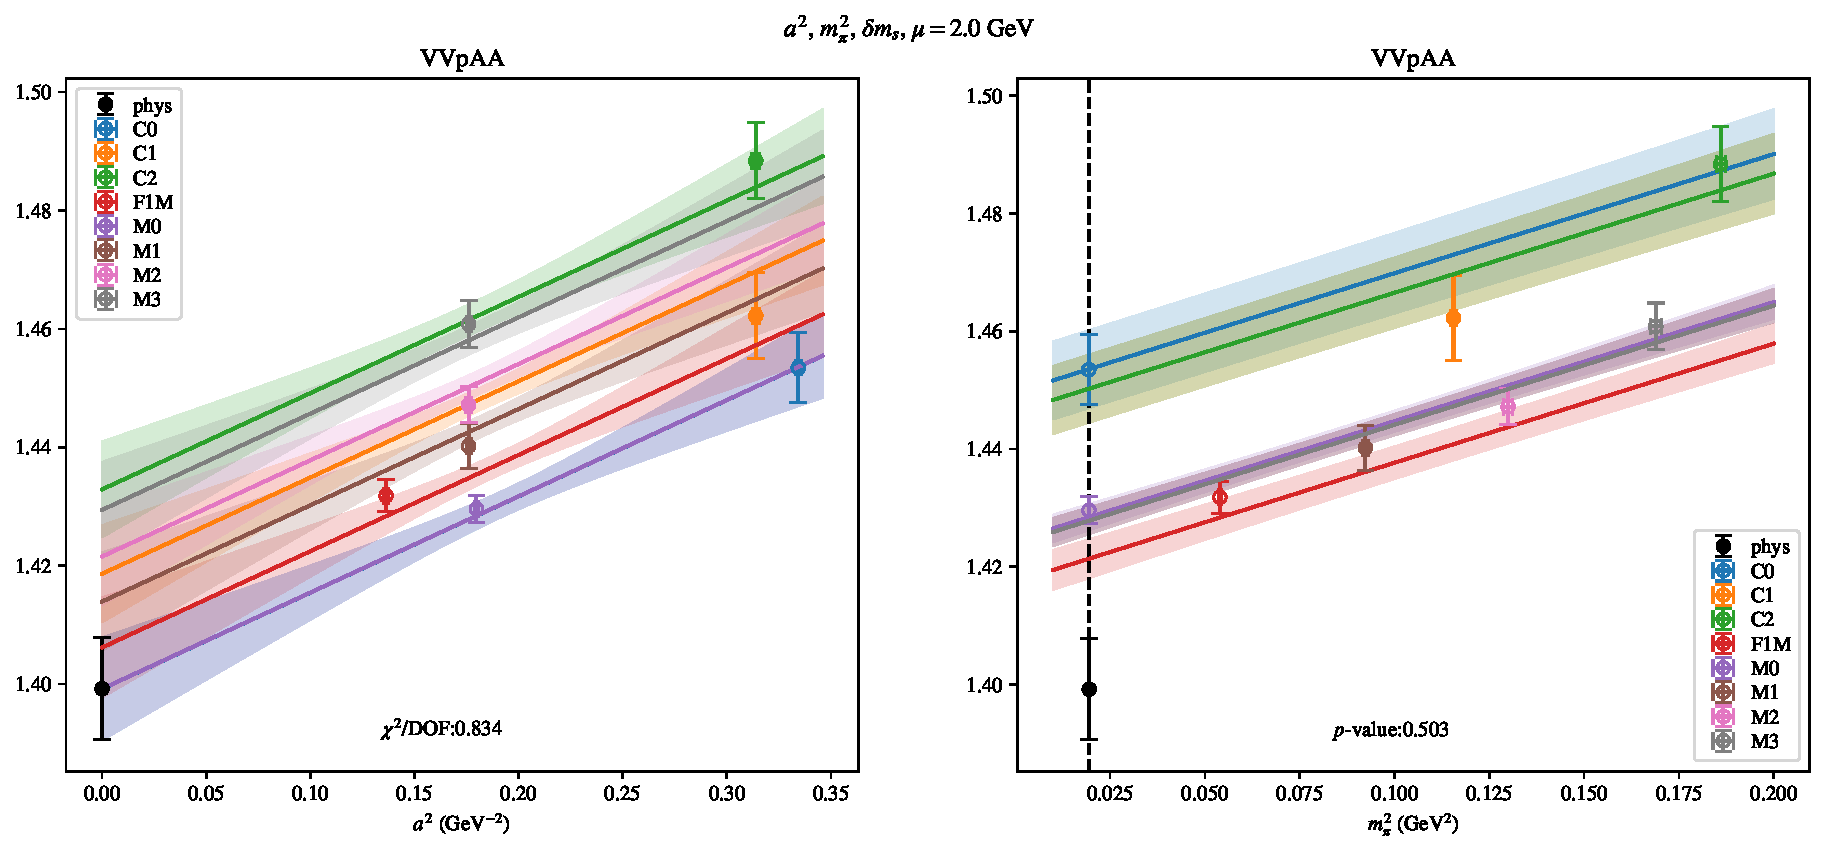
\includepdf[link, pages=-]{VVpAA/SUSY/a2m2delm_20.pdf}
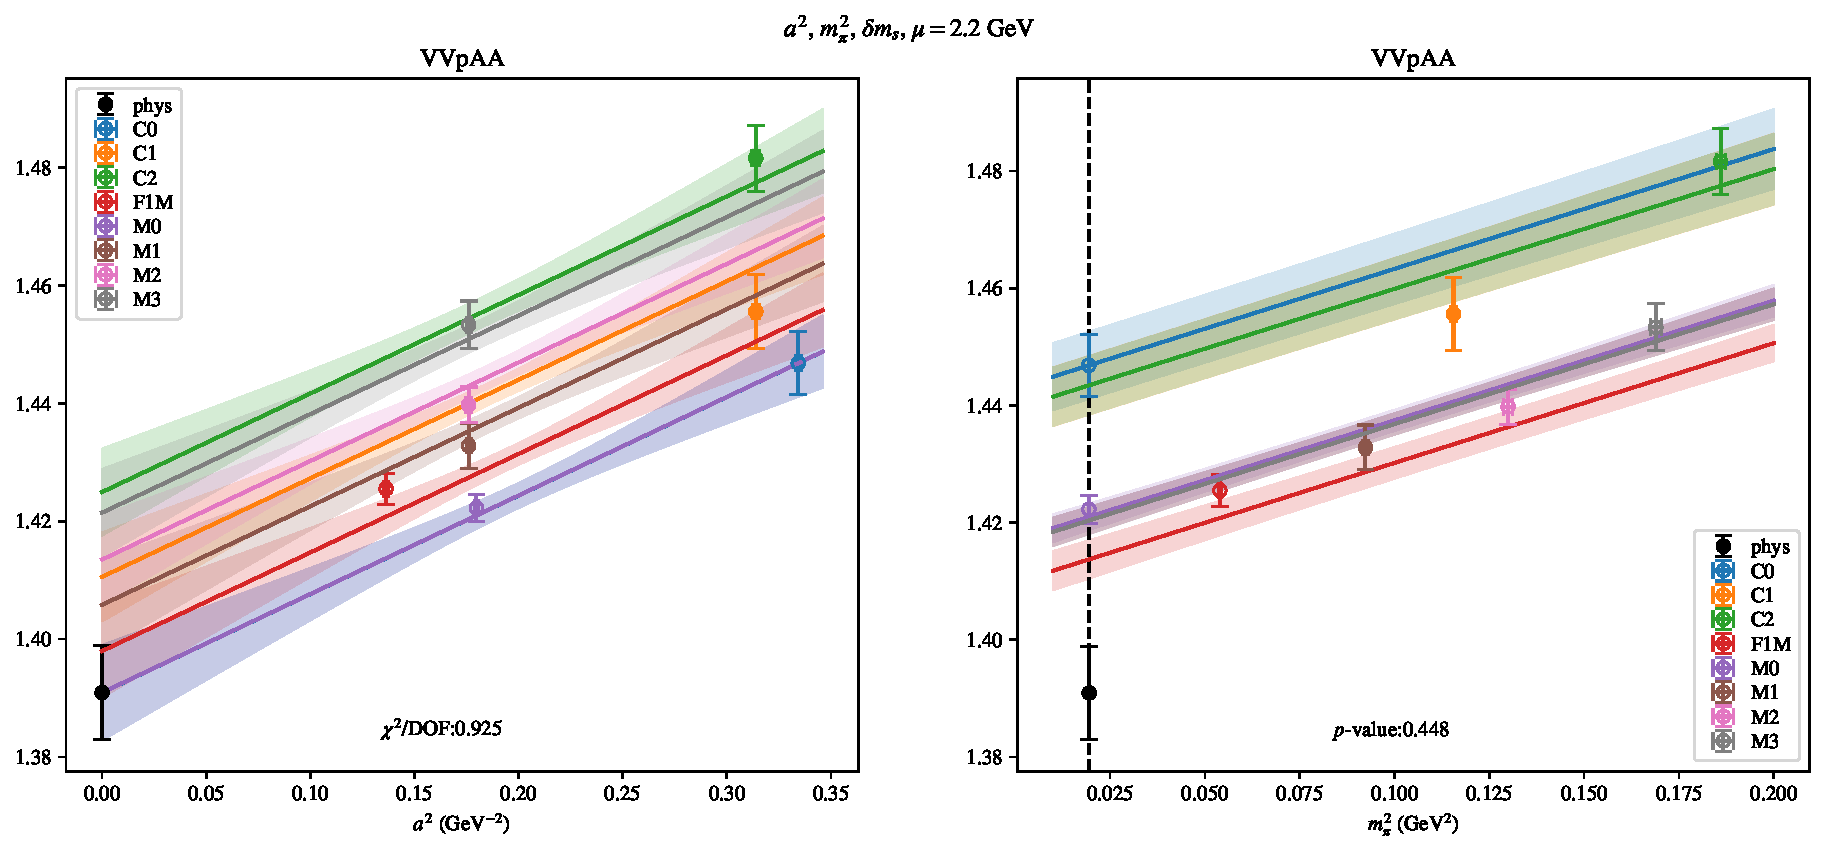
\includepdf[link, pages=-]{VVpAA/SUSY/a2m2delm_22.pdf}
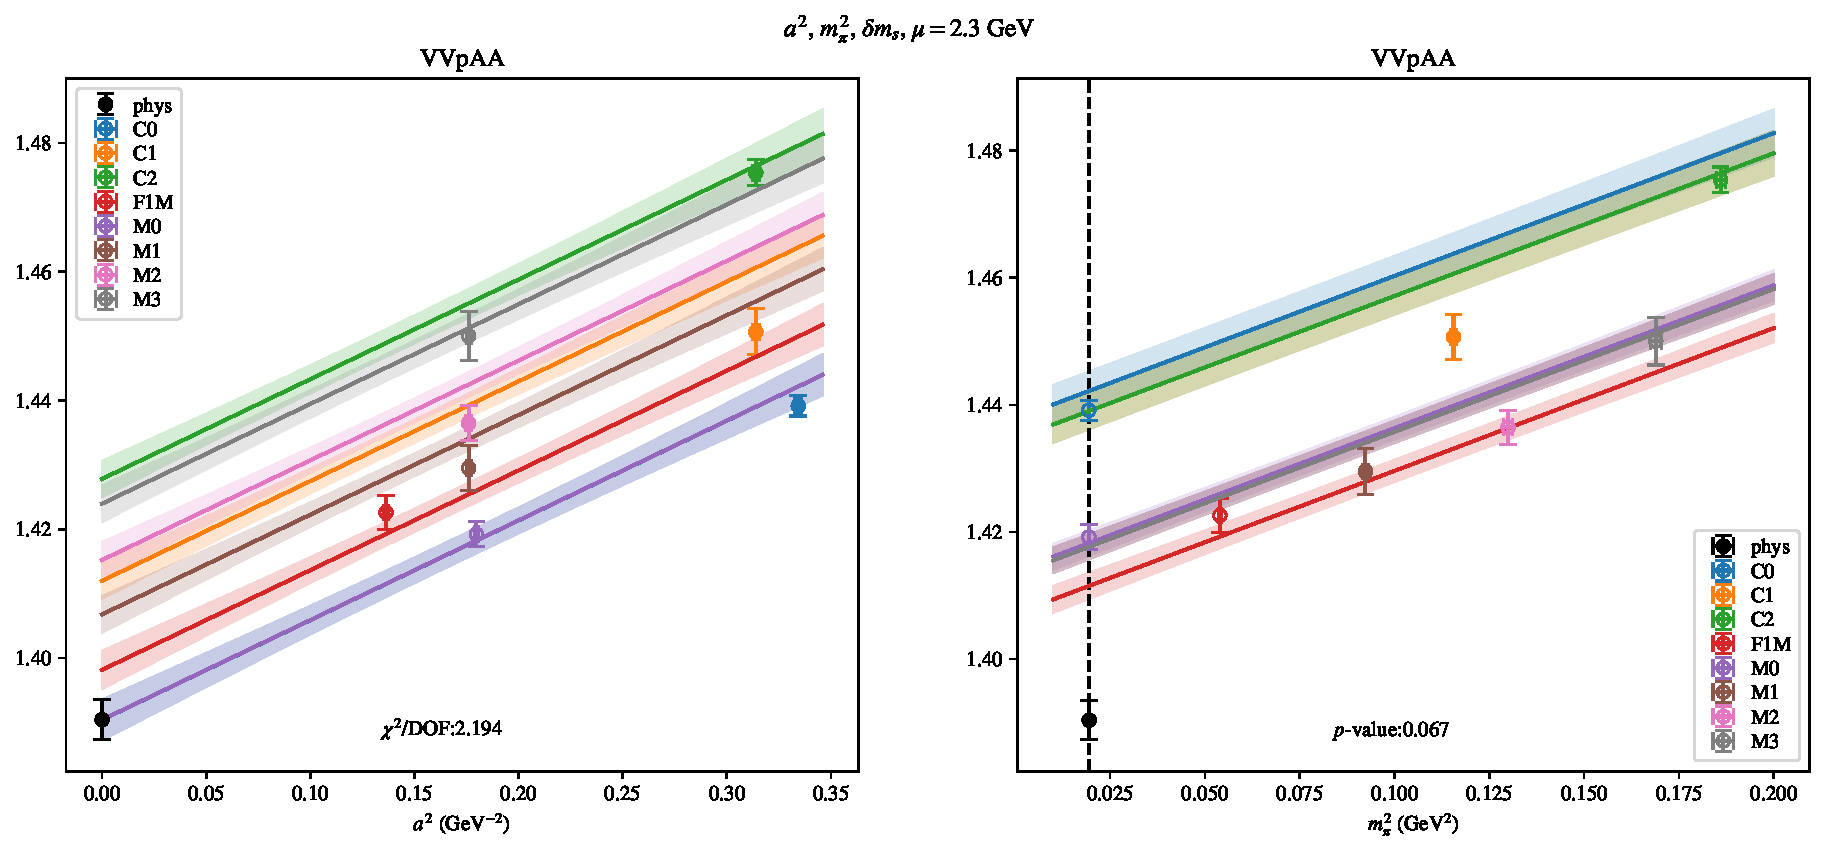
\includepdf[link, pages=-]{VVpAA/SUSY/a2m2delm_23.pdf}
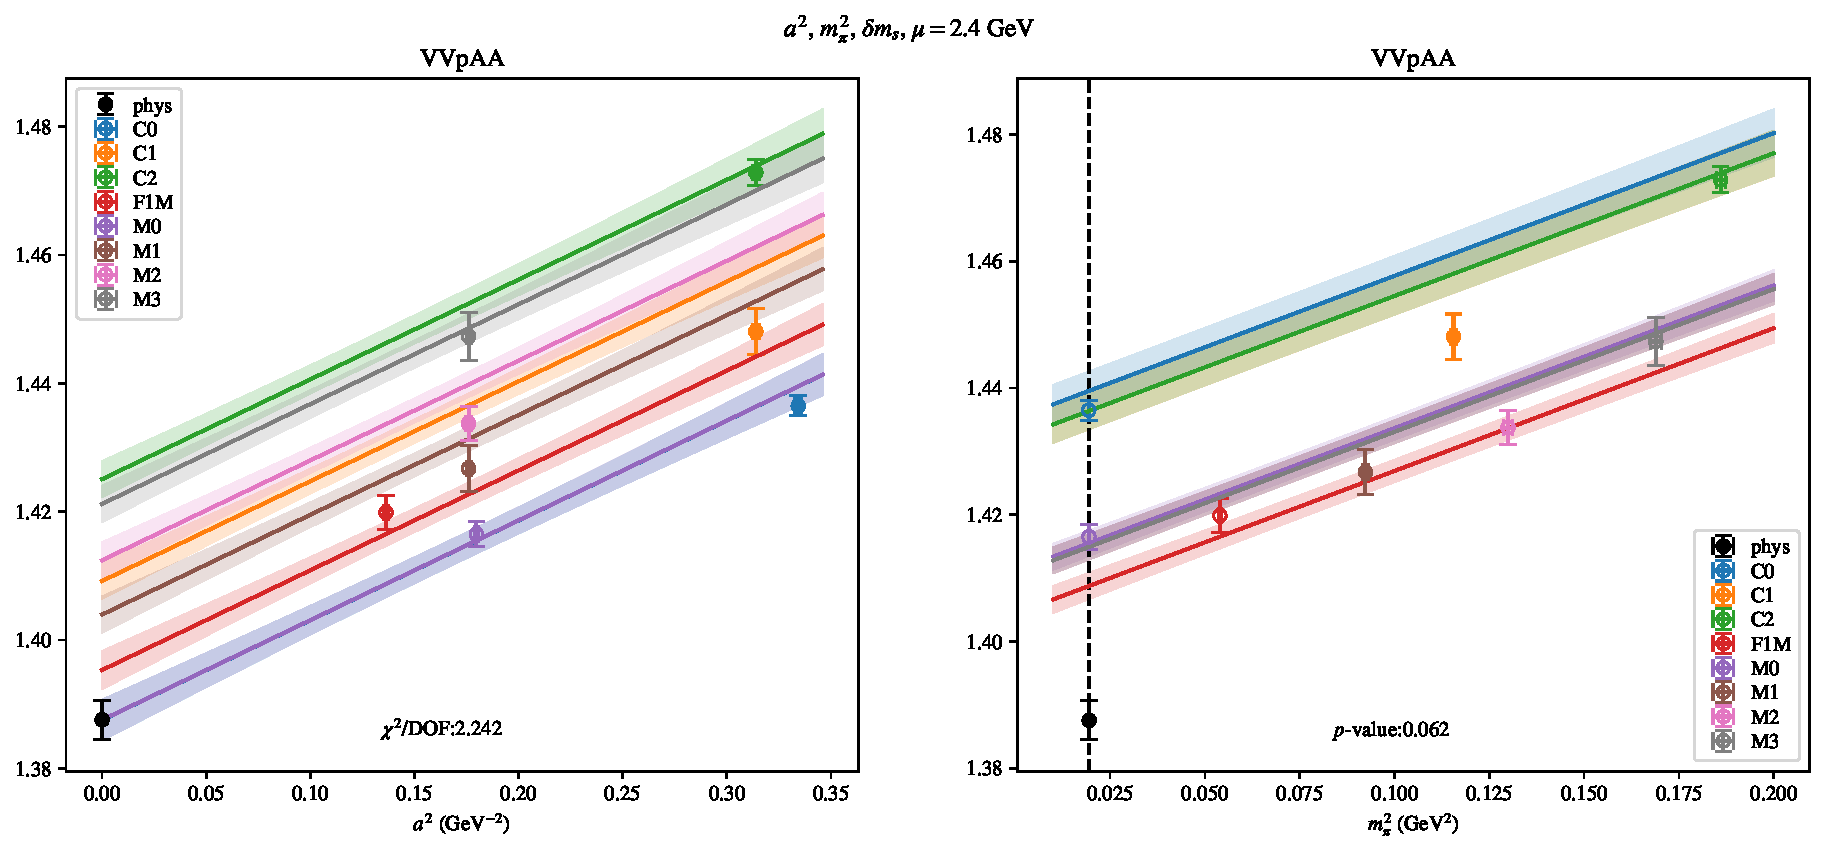
\includepdf[link, pages=-]{VVpAA/SUSY/a2m2delm_24.pdf}
\clearpage
\section{$\mathcal{B}_2$}
\begin{table}[h!]
\begin{center}
\begin{tabular}{|c|c|c|c|c|c|c|}
\hline
$\mu$ (GeV) & $a^2$, $m_\pi^2$& $a^2$, $m_\pi^2$ (no C)& $a^2$, $a^4$, $m_\pi^2$& $a^2$, $m_\pi^2$ (no M3, C2)& $a^2$, $m_\pi^2$, $m_\pi^4$& $a^2$, $m_\pi^2$, $\delta m_s$\\
\hline
2.0& \hyperlink{VVmAA/SUSY/a2m2_20.pdf.1}{\textbf{-0.925(17)}: 2.875 (0.013)} & \hyperlink{VVmAA/SUSY/a2m2noC_20.pdf.1}{\textbf{-0.936(97)}: 2.424 (0.089)} & \hyperlink{VVmAA/SUSY/a2a4m2_20.pdf.1}{\textbf{-0.92(16)}: 3.593 (0.006)} & \hyperlink{VVmAA/SUSY/a2m2mcut_20.pdf.1}{\textbf{-0.925(19)}: 3.107 (0.025)} & \hyperlink{VVmAA/SUSY/a2m2m4_20.pdf.1}{\textbf{-0.924(19)}: 2.585 (0.035)} & \hyperlink{VVmAA/SUSY/a2m2delm_20.pdf.1}{\textbf{-0.925(19)}: 3.479 (0.008)}\\
2.2& \hyperlink{VVmAA/SUSY/a2m2_22.pdf.1}{\textbf{-0.905(17)}: 3.935 (0.001)} & \hyperlink{VVmAA/SUSY/a2m2noC_22.pdf.1}{\textbf{-0.920(92)}: 1.943 (0.143)} & \hyperlink{VVmAA/SUSY/a2a4m2_22.pdf.1}{\textbf{-0.90(15)}: 4.919 (0.001)} & \hyperlink{VVmAA/SUSY/a2m2mcut_22.pdf.1}{\textbf{-0.906(19)}: 4.133 (0.006)} & \hyperlink{VVmAA/SUSY/a2m2m4_22.pdf.1}{\textbf{-0.904(18)}: 4.17 (0.002)} & \hyperlink{VVmAA/SUSY/a2m2delm_22.pdf.1}{\textbf{-0.905(19)}: 4.543 (0.001)}\\
2.3& \hyperlink{VVmAA/SUSY/a2m2_23.pdf.1}{\textbf{-0.897(17)}: 4.403 (0.001)} & \hyperlink{VVmAA/SUSY/a2m2noC_23.pdf.1}{\textbf{-0.913(91)}: 2.266 (0.104)} & \hyperlink{VVmAA/SUSY/a2a4m2_23.pdf.1}{\textbf{-0.89(15)}: 5.498 (0.0)} & \hyperlink{VVmAA/SUSY/a2m2mcut_23.pdf.1}{\textbf{-0.897(18)}: 4.799 (0.002)} & \hyperlink{VVmAA/SUSY/a2m2m4_23.pdf.1}{\textbf{-0.895(18)}: 4.573 (0.001)} & \hyperlink{VVmAA/SUSY/a2m2delm_23.pdf.1}{\textbf{-0.896(18)}: 4.999 (0.001)}\\
2.4& \hyperlink{VVmAA/SUSY/a2m2_24.pdf.1}{\textbf{-0.889(17)}: 4.798 (0.0)} & \hyperlink{VVmAA/SUSY/a2m2noC_24.pdf.1}{\textbf{-0.906(90)}: 2.421 (0.089)} & \hyperlink{VVmAA/SUSY/a2a4m2_24.pdf.1}{\textbf{-0.89(15)}: 5.994 (0.0)} & \hyperlink{VVmAA/SUSY/a2m2mcut_24.pdf.1}{\textbf{-0.890(18)}: 5.37 (0.001)} & \hyperlink{VVmAA/SUSY/a2m2m4_24.pdf.1}{\textbf{-0.888(18)}: 5.094 (0.0)} & \hyperlink{VVmAA/SUSY/a2m2delm_24.pdf.1}{\textbf{-0.888(18)}: 5.458 (0.0)}\\
\hline
\end{tabular}
\caption{Physical point value from chiral and continuum extrapolation at renormalisation scale $\mu$. Entries are \textbf{value(error)}: $\chi^2/\text{DOF}$ ($p$-value).}
\end{center}
\end{table}
\begin{table}[h!]
\begin{center}
\begin{tabular}{|c c|c|c|c|c|c|c|}
\hline
$\mu$ (GeV) &  & $a^2$, $m_\pi^2$& $a^2$, $m_\pi^2$ (no C)& $a^2$, $a^4$, $m_\pi^2$& $a^2$, $m_\pi^2$ (no M3, C2)& $a^2$, $m_\pi^2$, $m_\pi^4$& $a^2$, $m_\pi^2$, $\delta m_s$\\
\hline
\multirow{2}{0.5in}{2.0} & $\alpha$ & 0.3752(79)& 0.308(63)& 0.37(16)& 0.3751(87)& 0.3808(87)& 0.3770(86)\\
 & $\beta$ & 0.00666(16)& 0.00614(28)& 0.00666(17)& 0.00706(26)& 0.00835(79)& 0.00669(17)\\
\hline
\multirow{2}{0.5in}{2.2} & $\alpha$ & 0.4225(80)& 0.329(61)& 0.42(16)& 0.4191(88)& 0.4273(87)& 0.4257(87)\\
 & $\beta$ & 0.00706(15)& 0.00635(24)& 0.00706(17)& 0.00739(25)& 0.00845(74)& 0.00712(16)\\
\hline
\multirow{2}{0.5in}{2.3} & $\alpha$ & 0.4442(81)& 0.338(61)& 0.42(16)& 0.4411(89)& 0.4497(88)& 0.4477(88)\\
 & $\beta$ & 0.00715(15)& 0.00644(23)& 0.00714(17)& 0.00750(25)& 0.00867(74)& 0.00722(16)\\
\hline
\multirow{2}{0.5in}{2.4} & $\alpha$ & 0.4632(82)& 0.354(61)& 0.44(16)& 0.4598(90)& 0.4688(89)& 0.4668(88)\\
 & $\beta$ & 0.00725(15)& 0.00651(22)& 0.00724(17)& 0.00756(25)& 0.00872(74)& 0.00732(16)\\
\hline
\end{tabular}
\caption{Fit values of coefficients in $Q = Q_{phys} + \mathbf{\alpha} a^2 + \mathbf{\beta}\left(\frac{m_\pi^2}{f_\pi^2}-\frac{m_{\pi,PDG}^2}{f_\pi^2}\right) + \ldots$.}
\end{center}
\end{table}
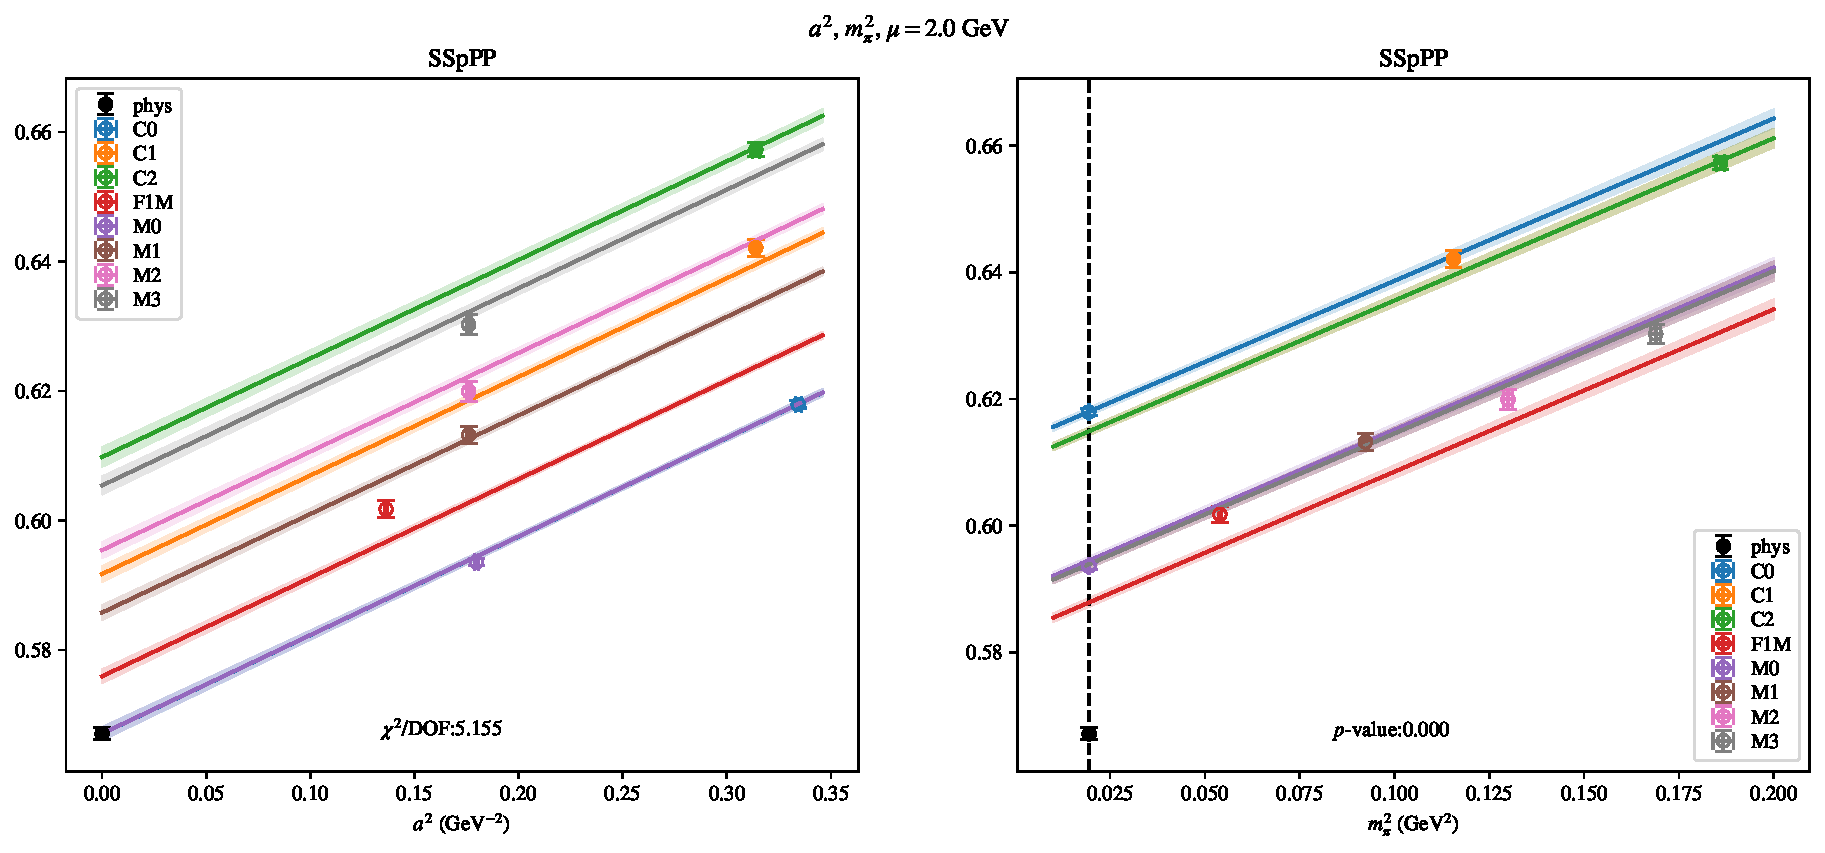
\includepdf[link, pages=-]{VVmAA/SUSY/a2m2_20.pdf}
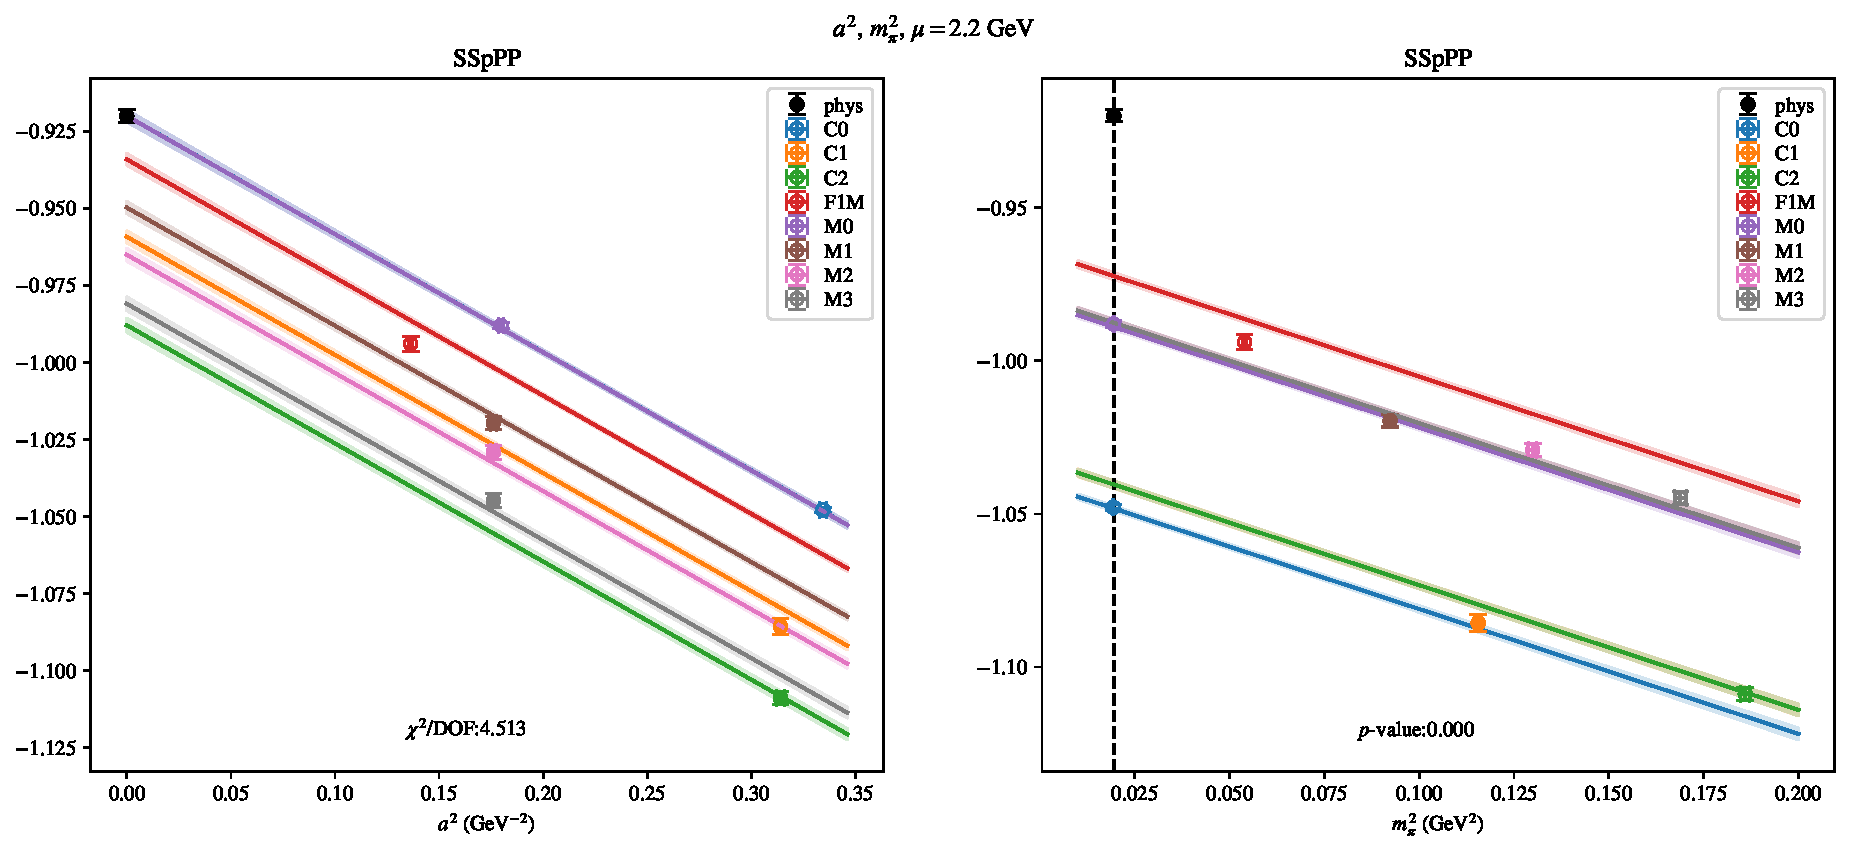
\includepdf[link, pages=-]{VVmAA/SUSY/a2m2_22.pdf}
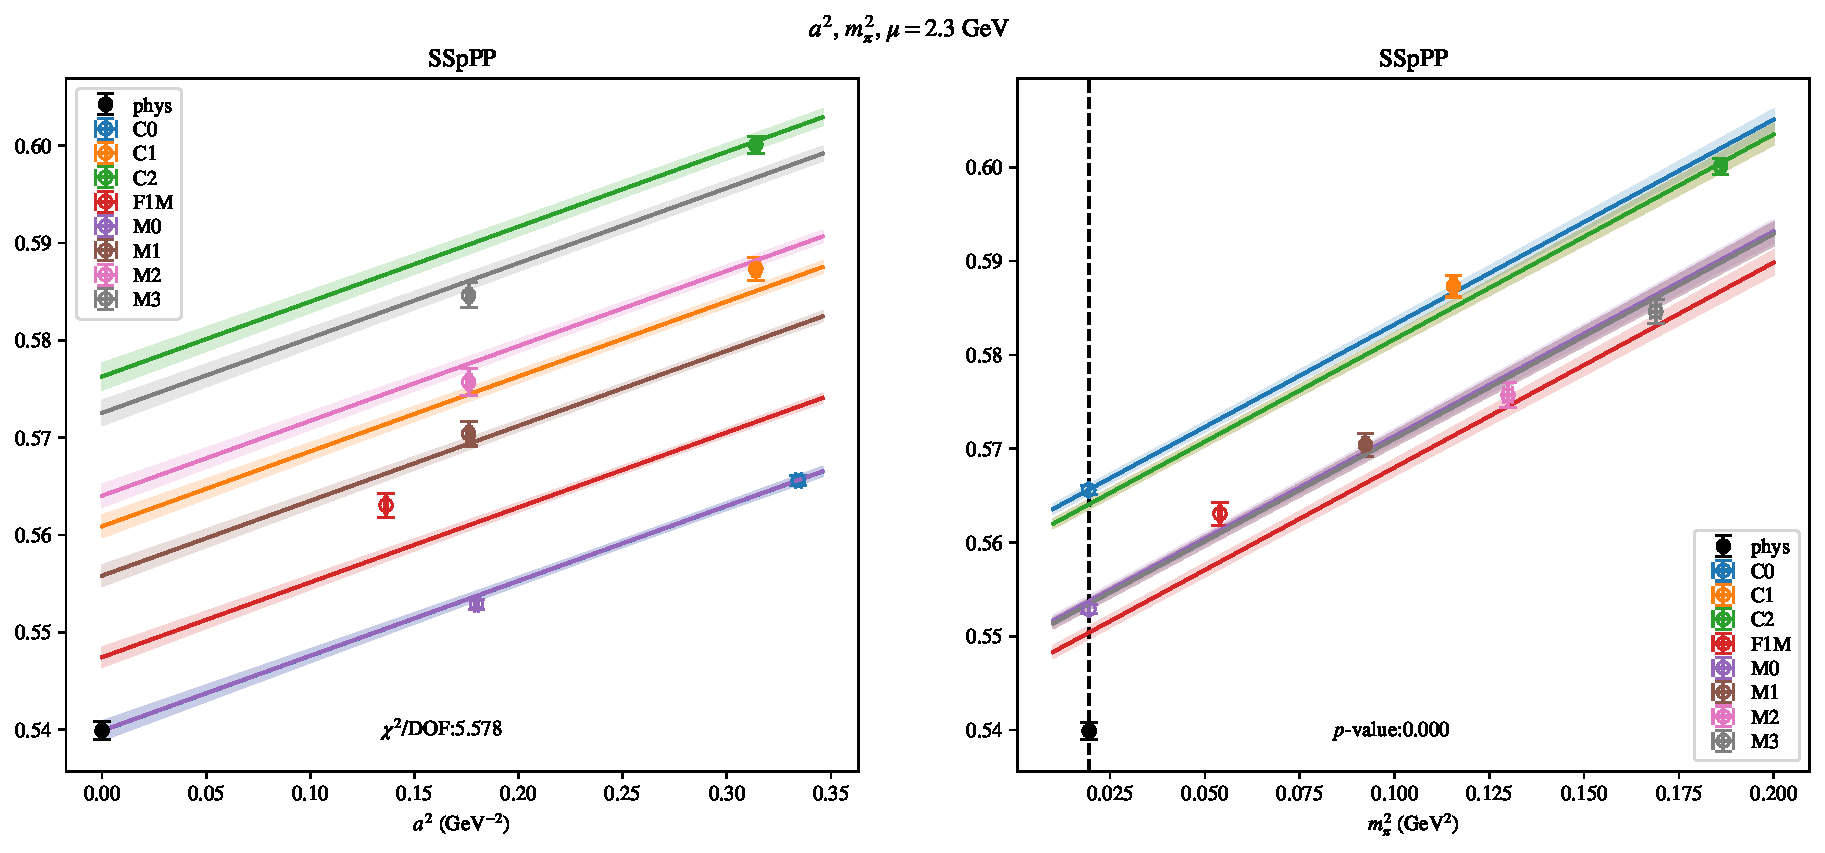
\includepdf[link, pages=-]{VVmAA/SUSY/a2m2_23.pdf}
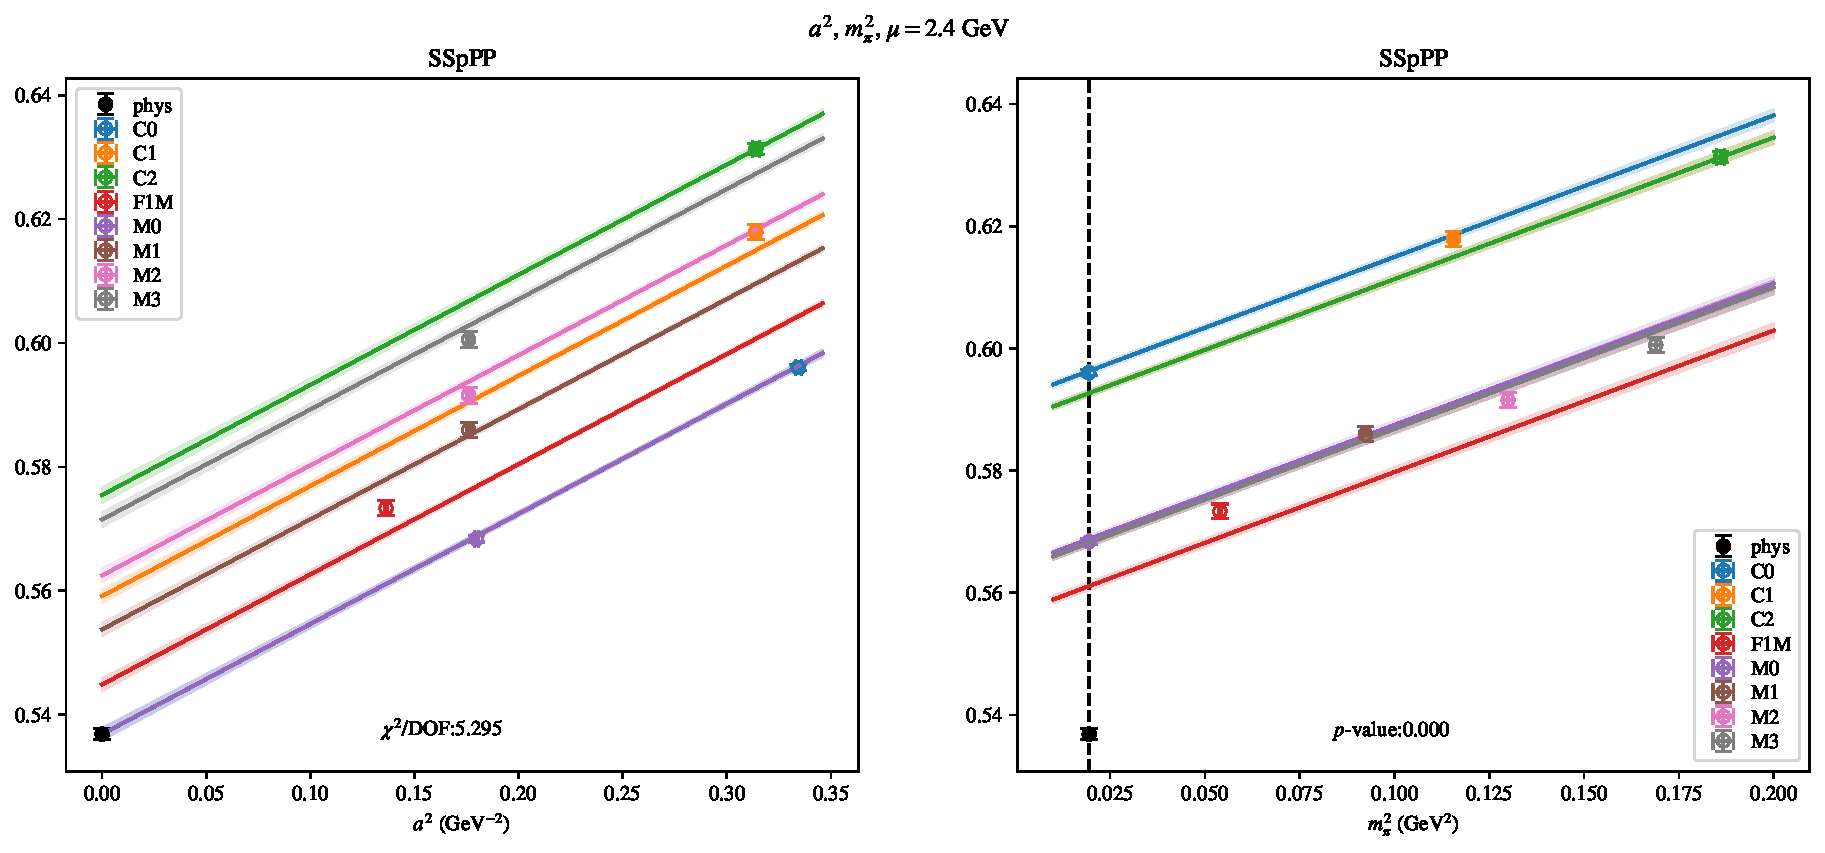
\includepdf[link, pages=-]{VVmAA/SUSY/a2m2_24.pdf}
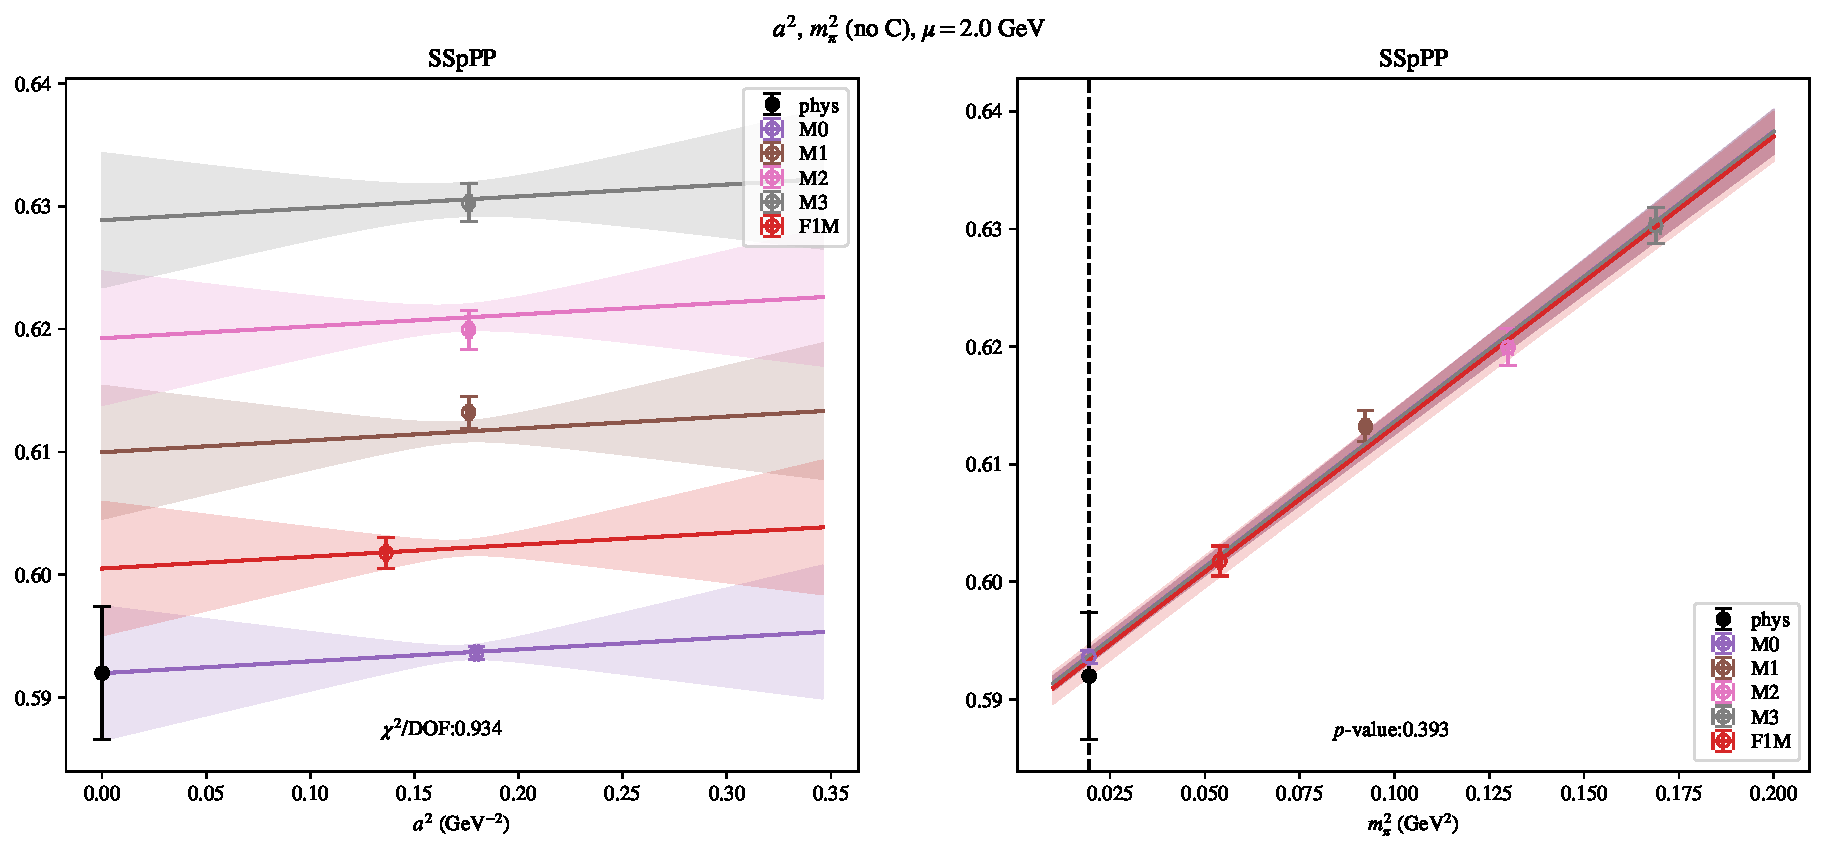
\includepdf[link, pages=-]{VVmAA/SUSY/a2m2noC_20.pdf}
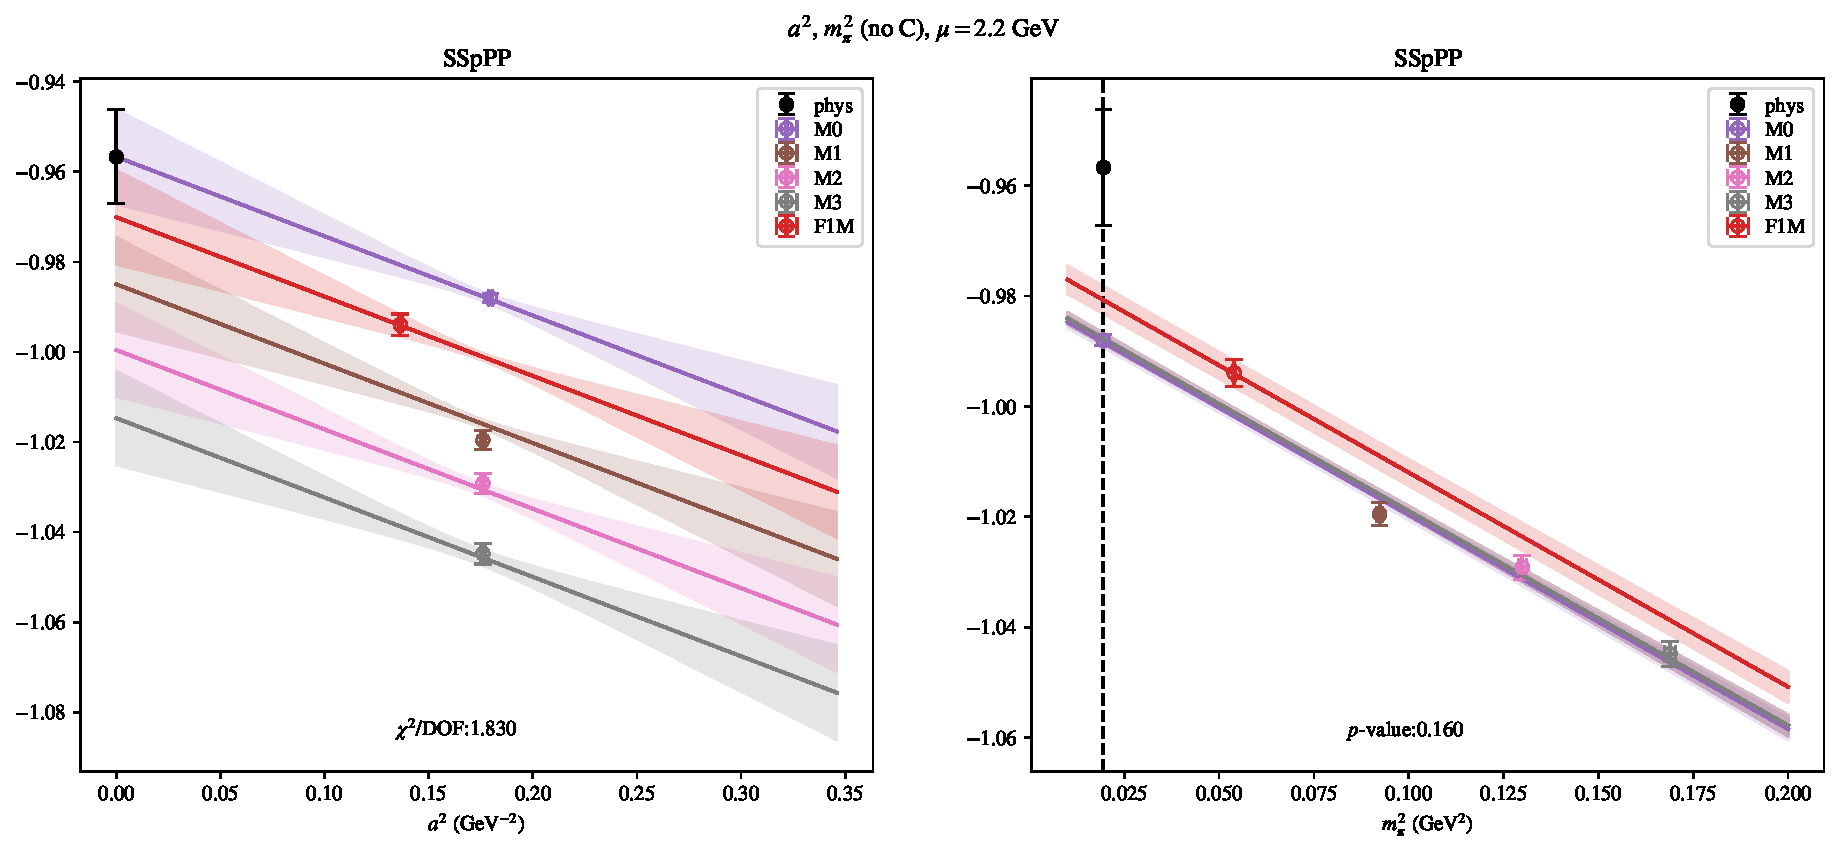
\includepdf[link, pages=-]{VVmAA/SUSY/a2m2noC_22.pdf}
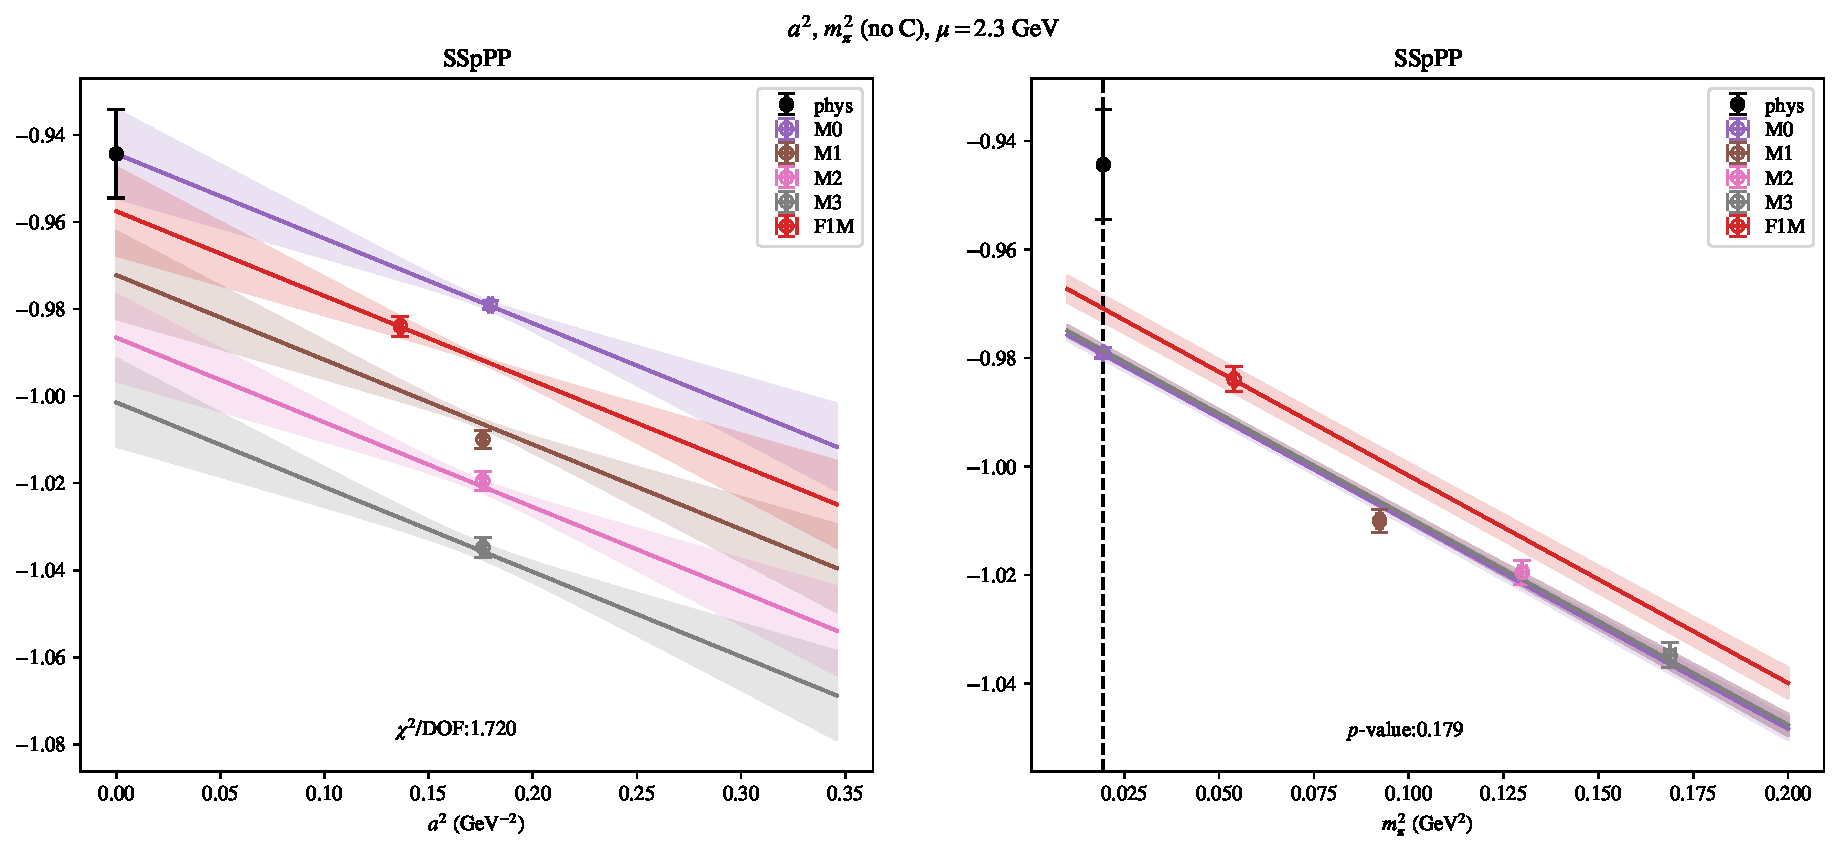
\includepdf[link, pages=-]{VVmAA/SUSY/a2m2noC_23.pdf}
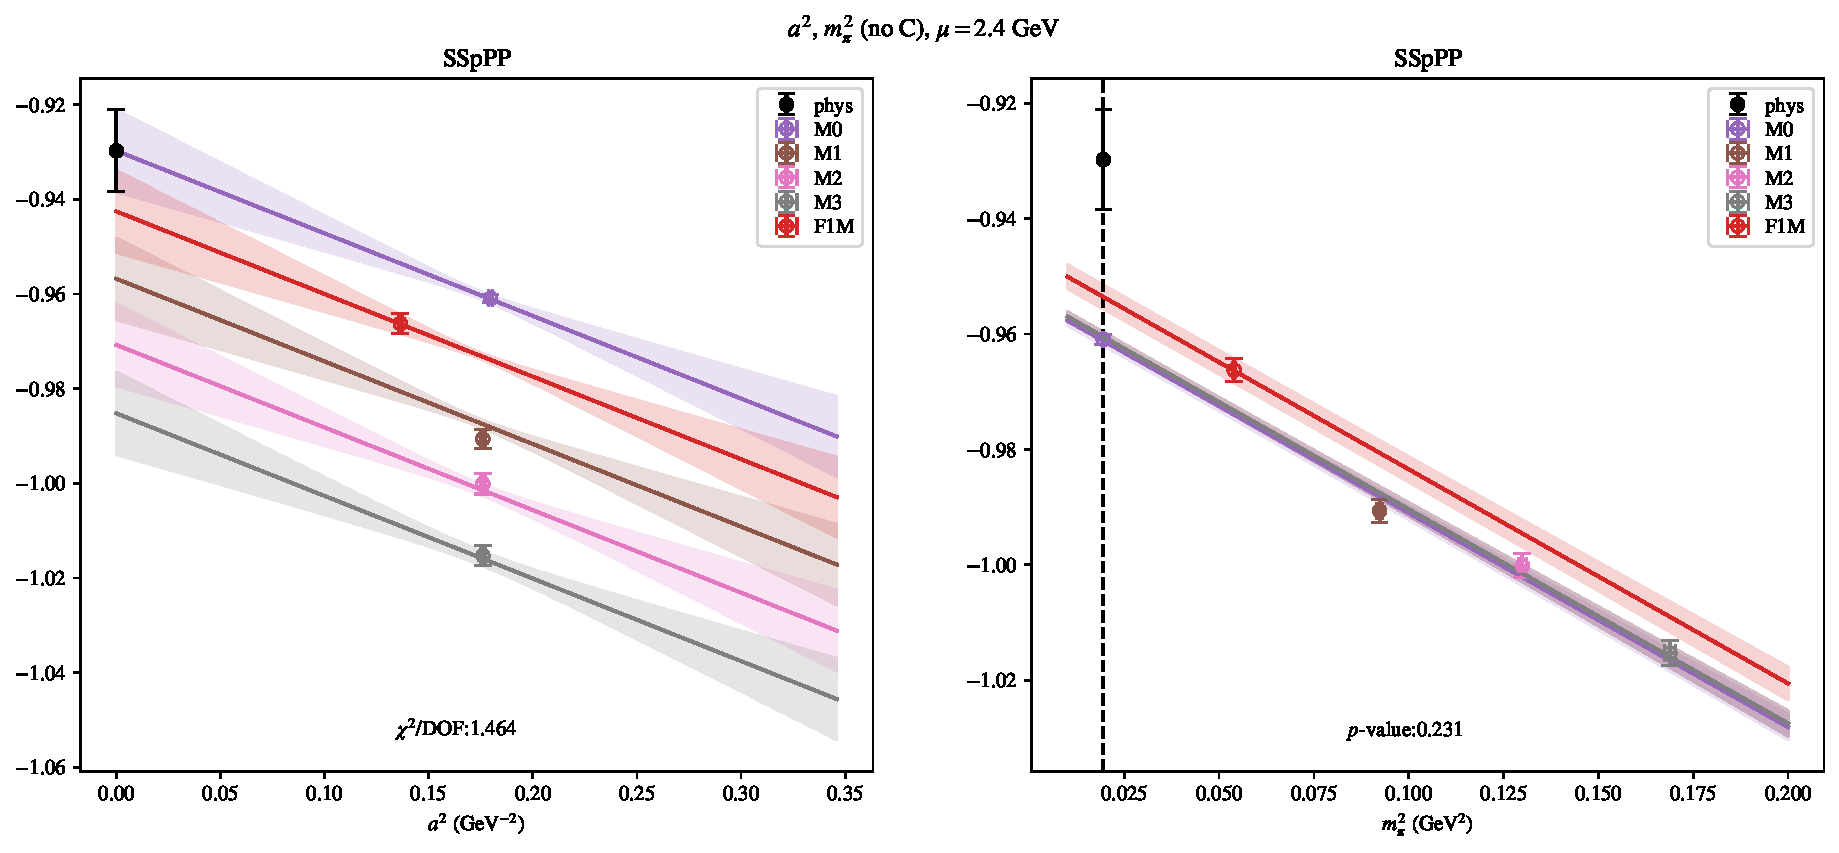
\includepdf[link, pages=-]{VVmAA/SUSY/a2m2noC_24.pdf}
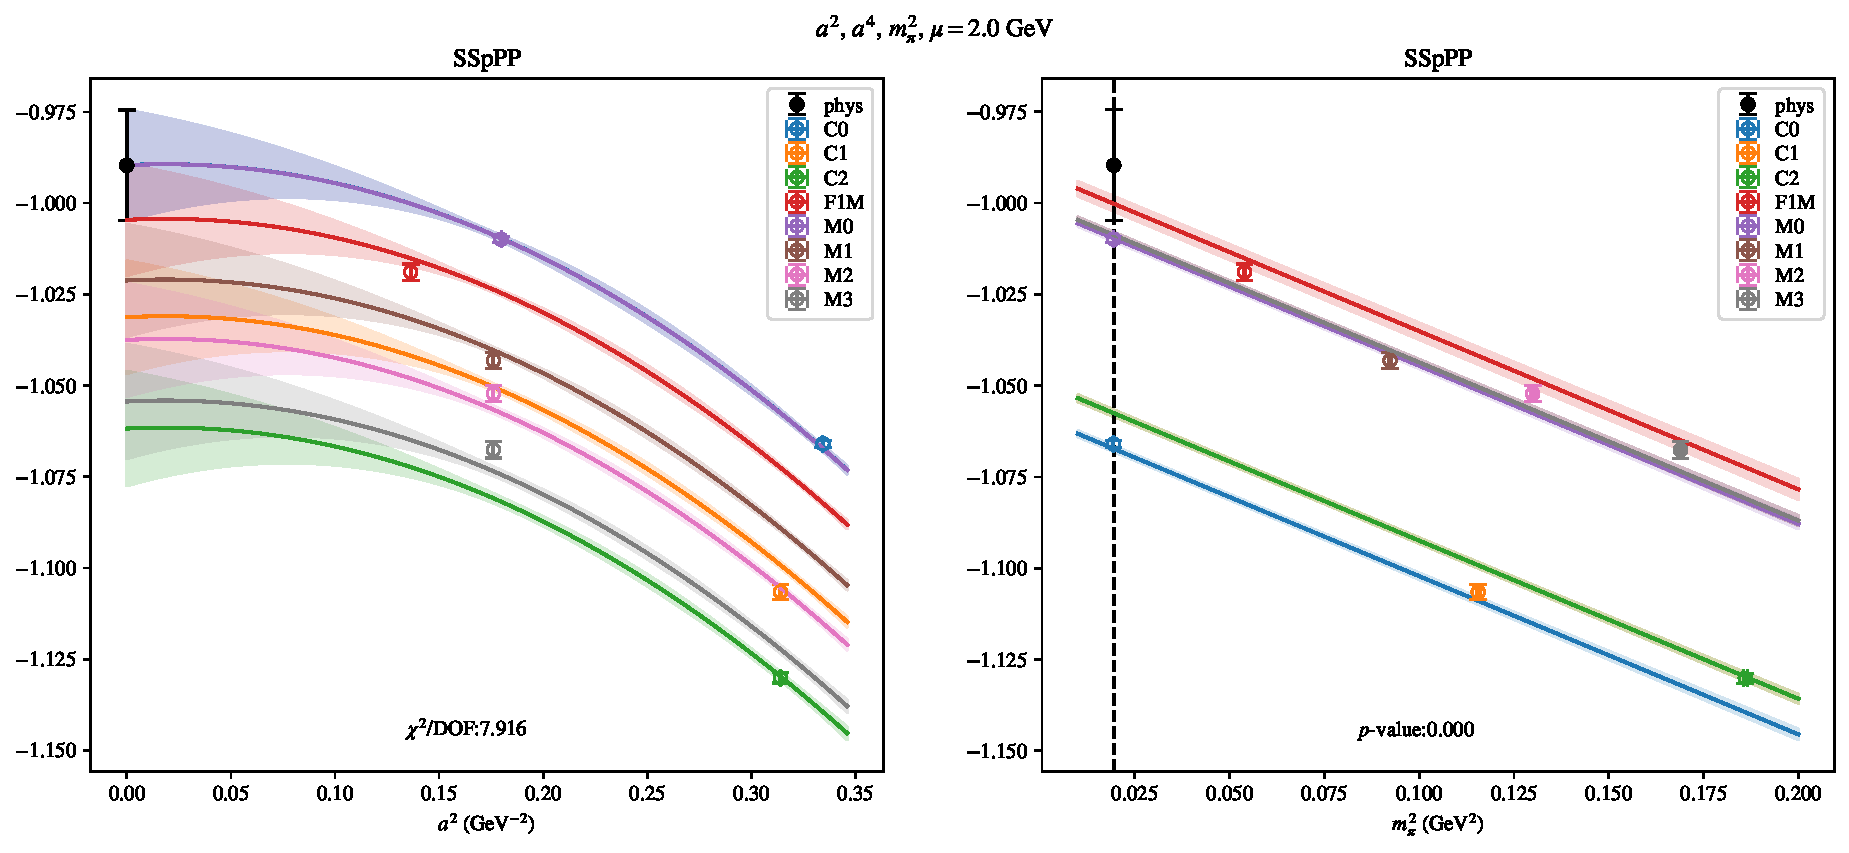
\includepdf[link, pages=-]{VVmAA/SUSY/a2a4m2_20.pdf}
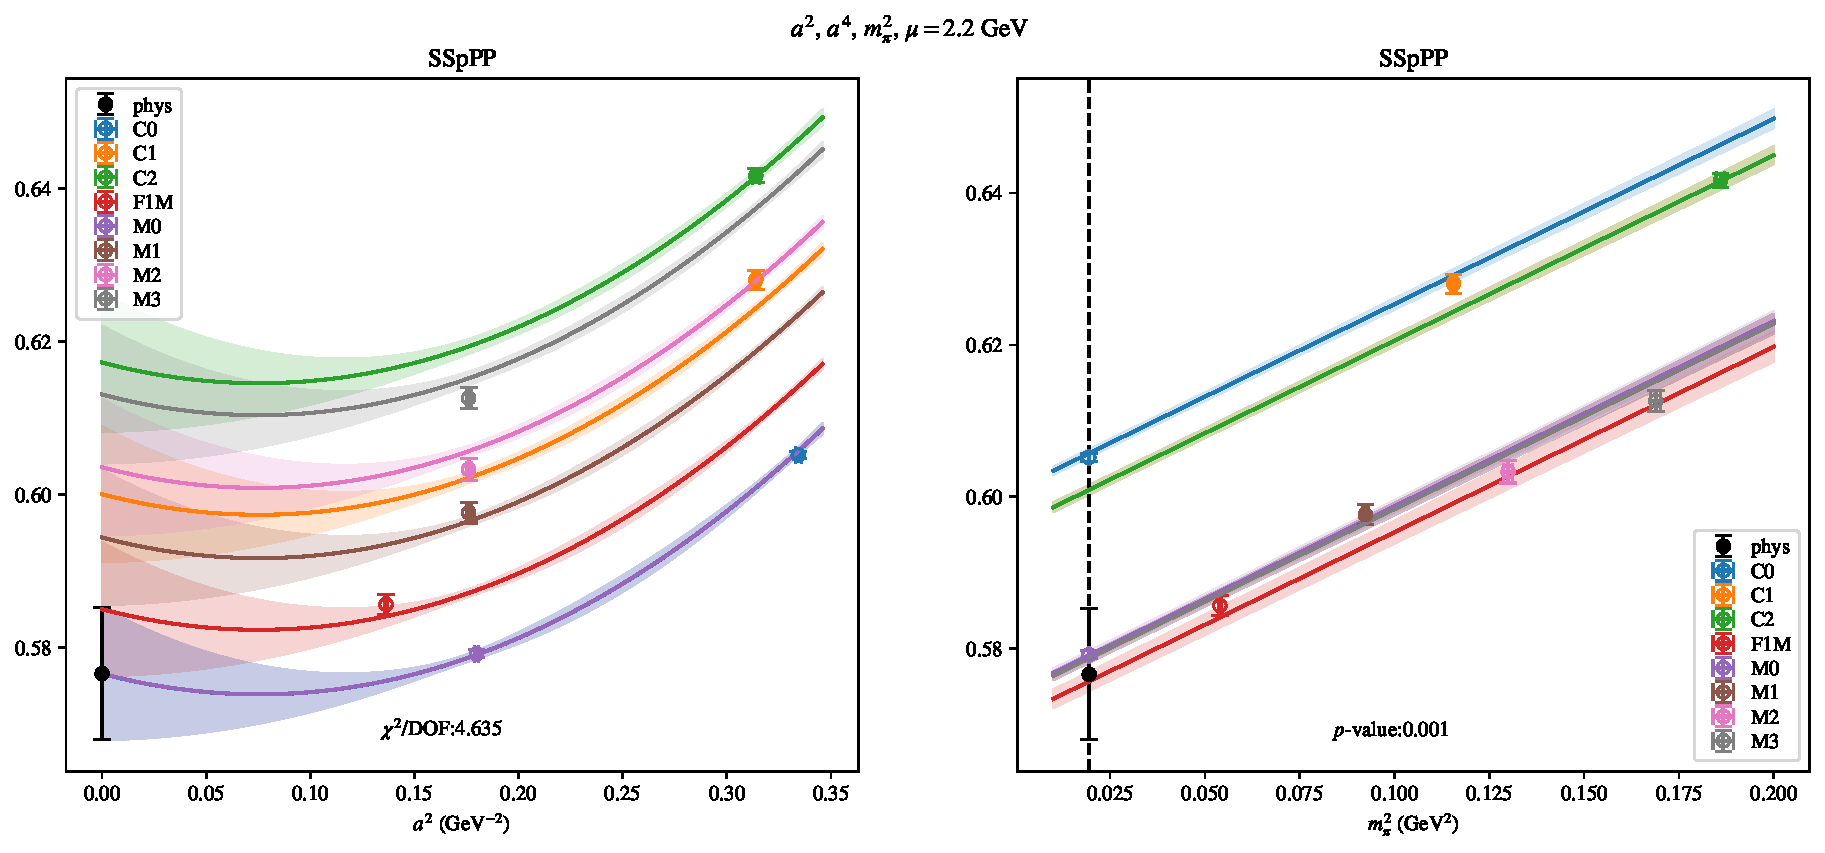
\includepdf[link, pages=-]{VVmAA/SUSY/a2a4m2_22.pdf}
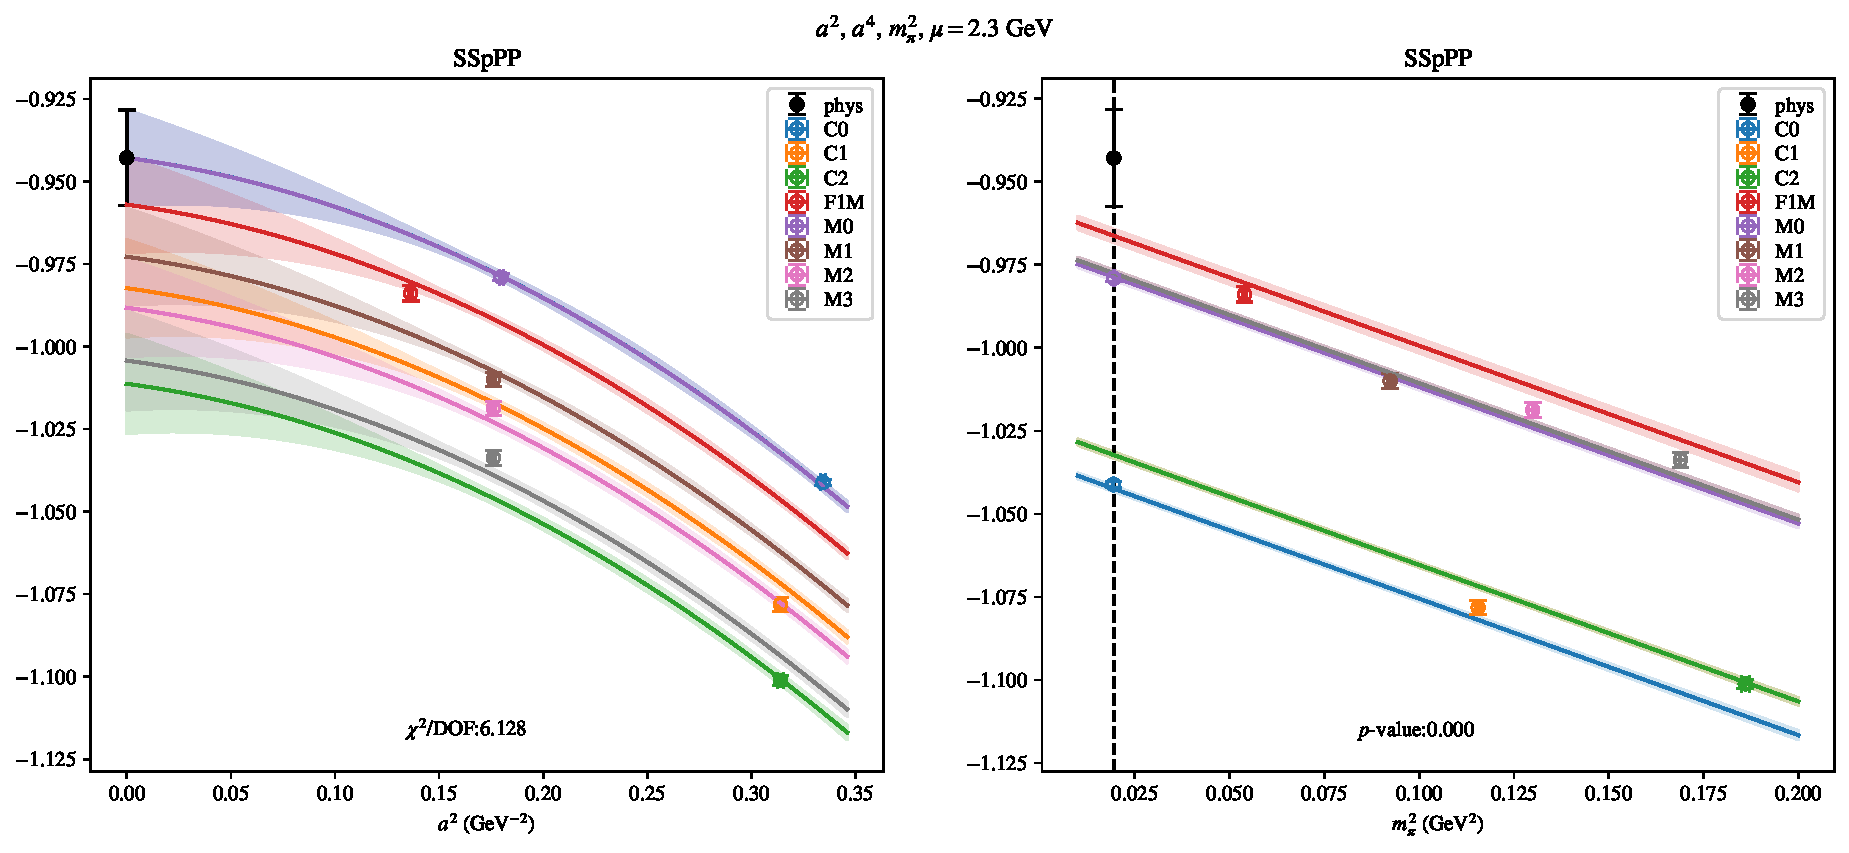
\includepdf[link, pages=-]{VVmAA/SUSY/a2a4m2_23.pdf}
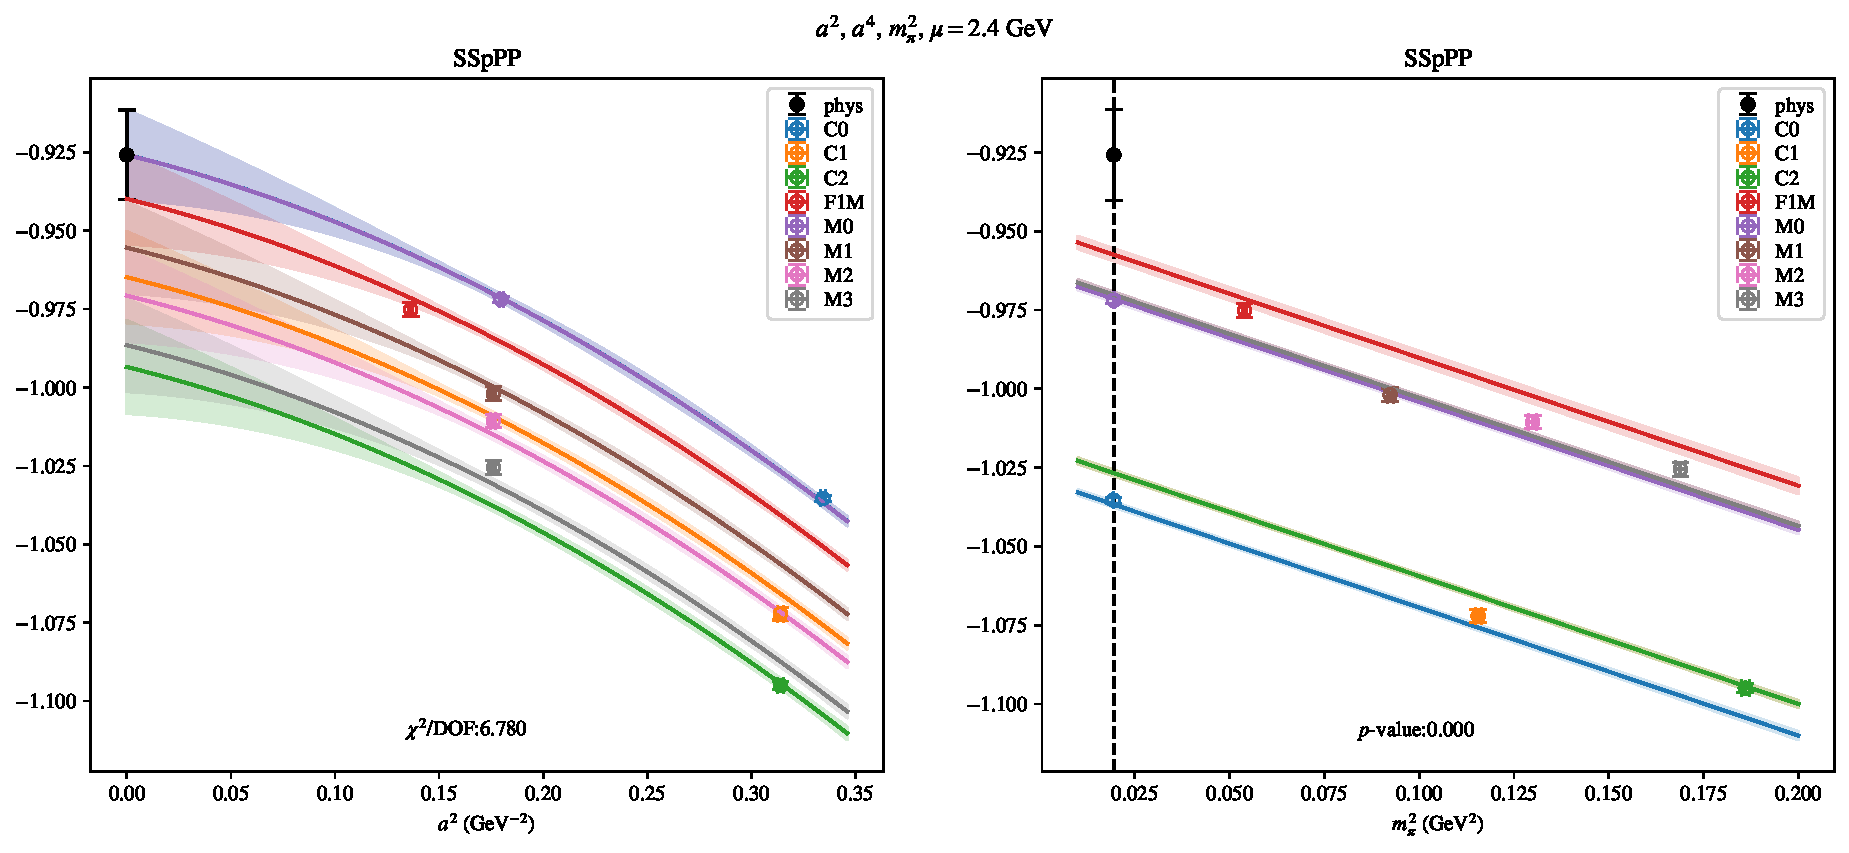
\includepdf[link, pages=-]{VVmAA/SUSY/a2a4m2_24.pdf}
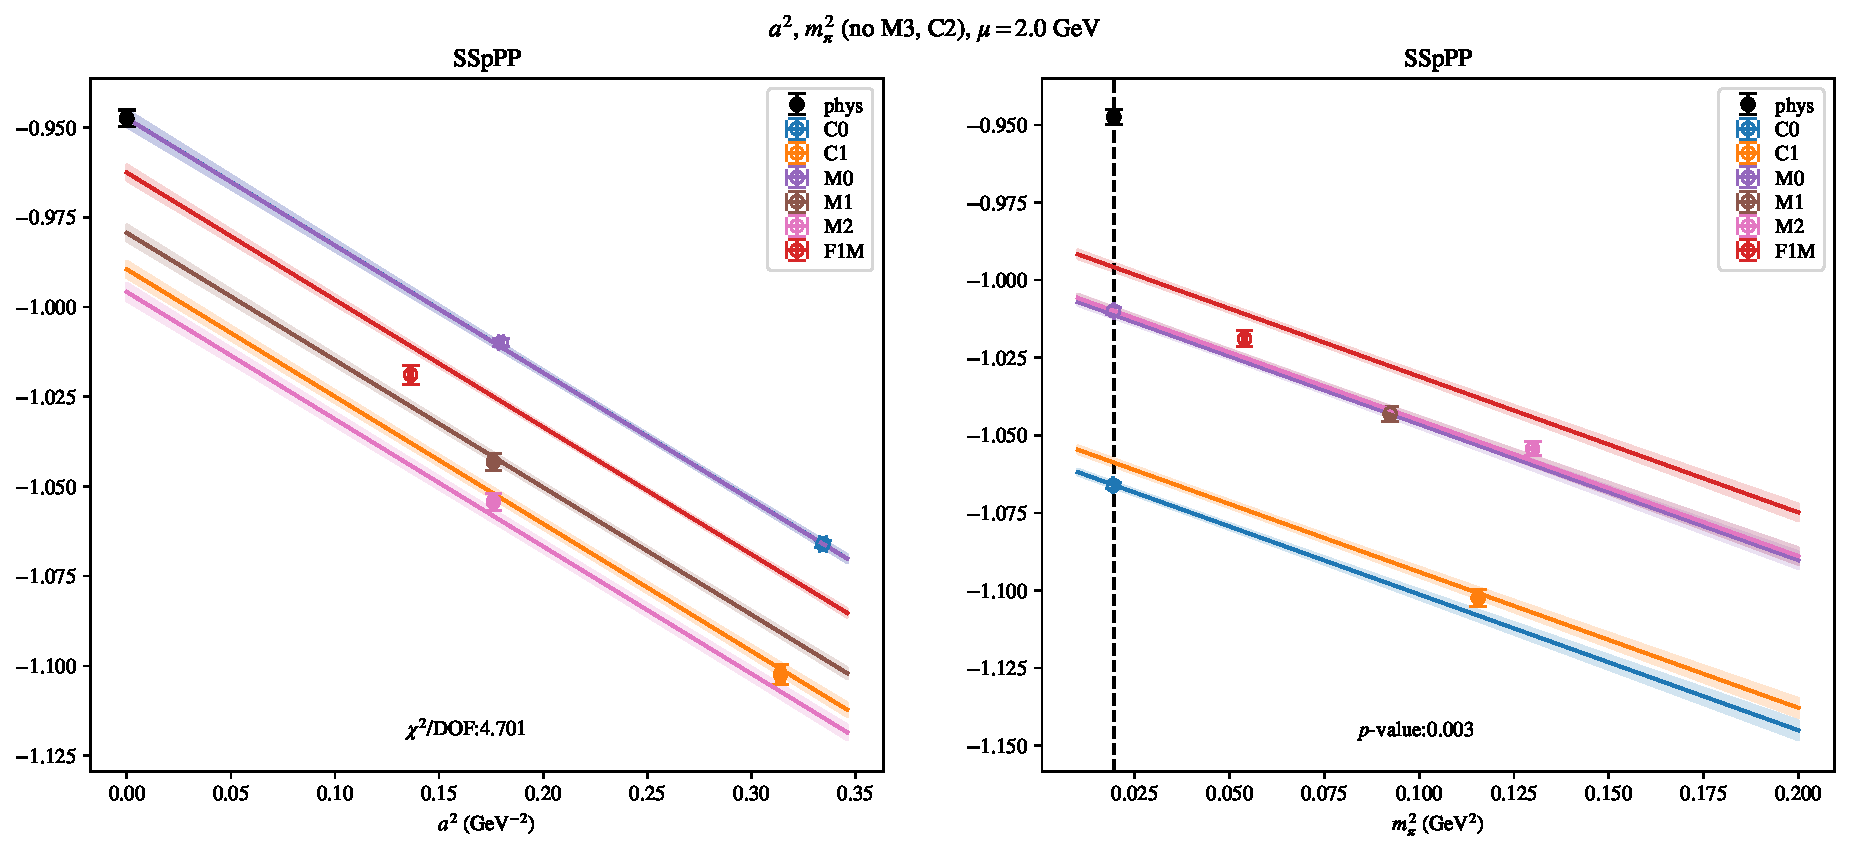
\includepdf[link, pages=-]{VVmAA/SUSY/a2m2mcut_20.pdf}
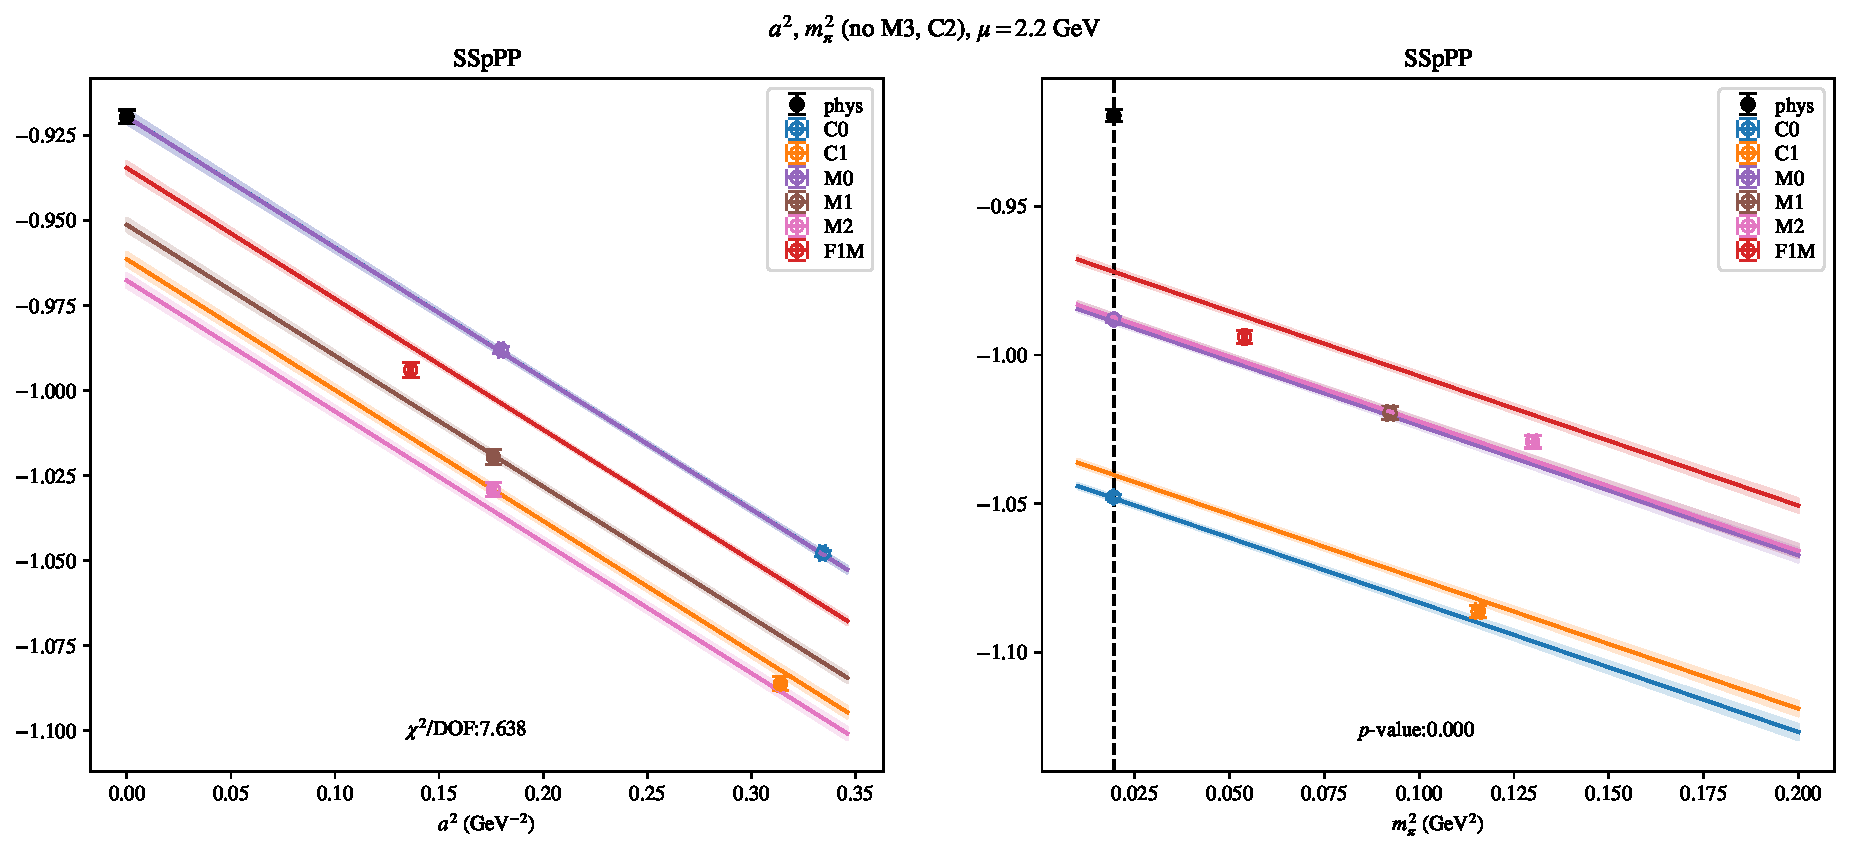
\includepdf[link, pages=-]{VVmAA/SUSY/a2m2mcut_22.pdf}
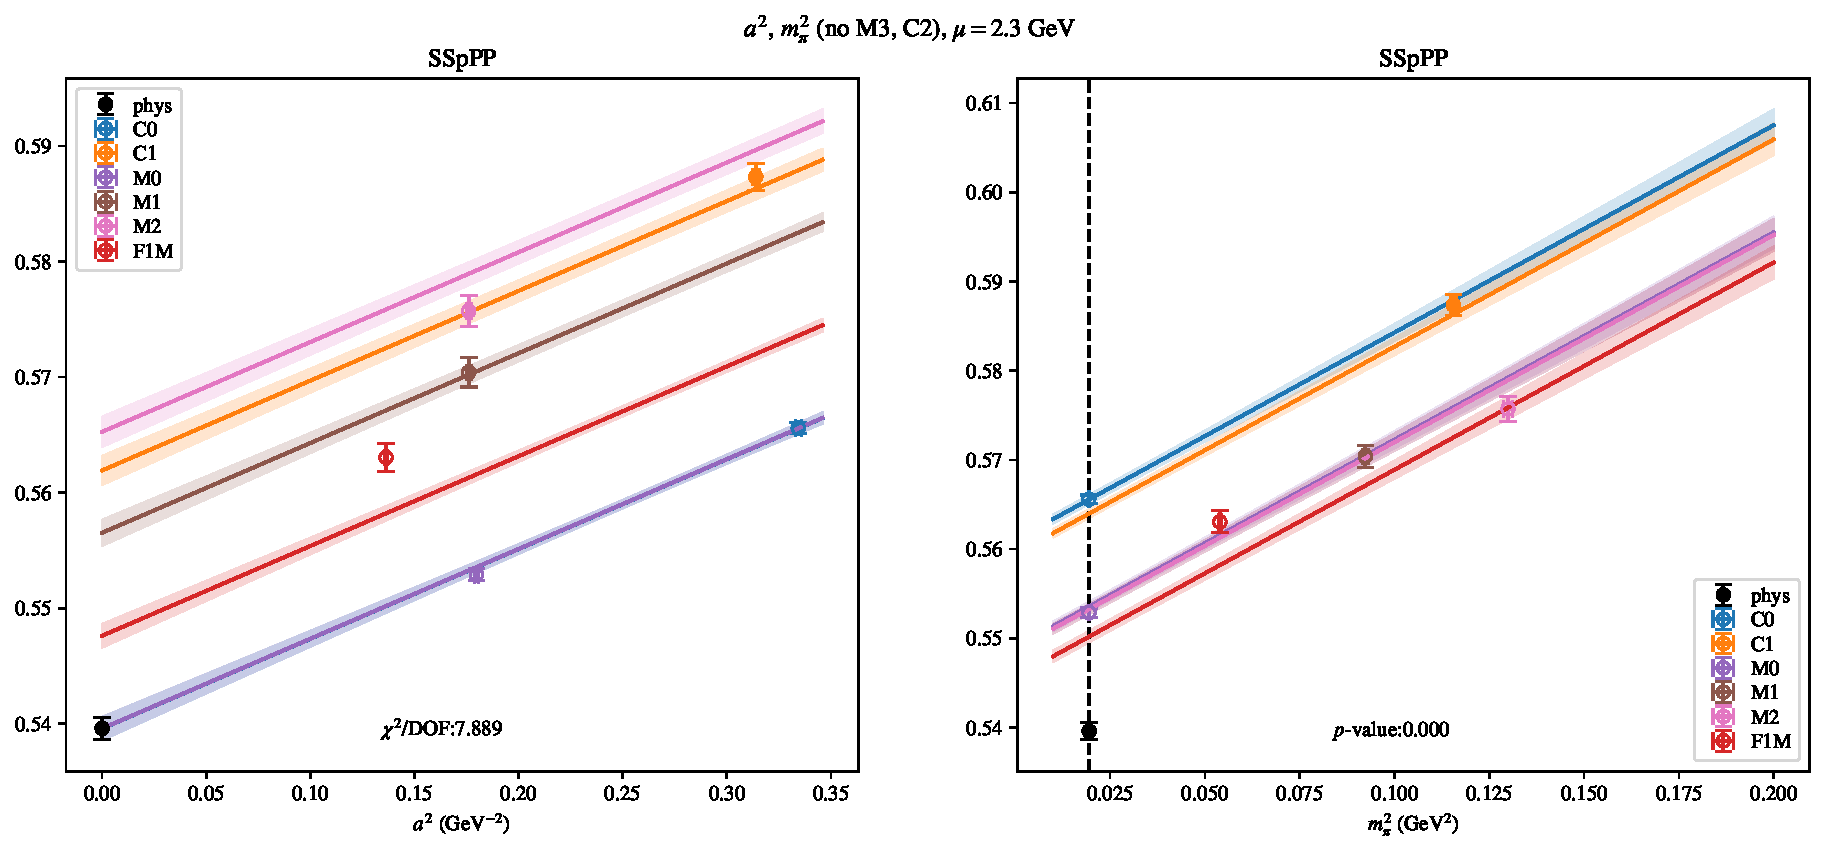
\includepdf[link, pages=-]{VVmAA/SUSY/a2m2mcut_23.pdf}
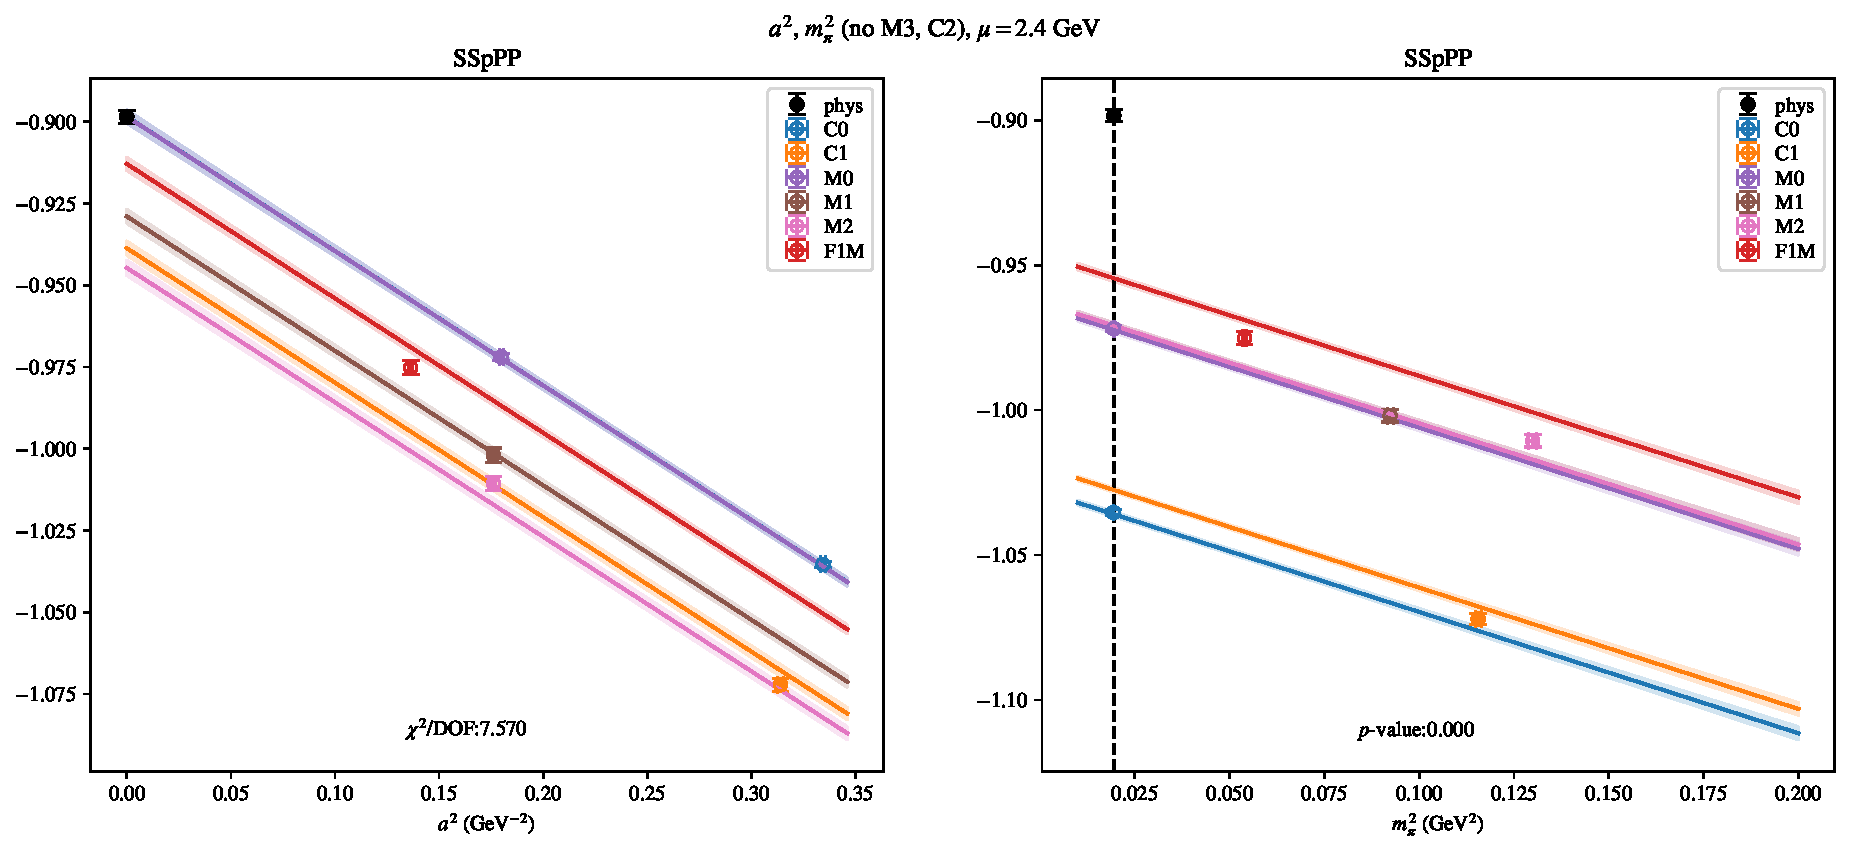
\includepdf[link, pages=-]{VVmAA/SUSY/a2m2mcut_24.pdf}
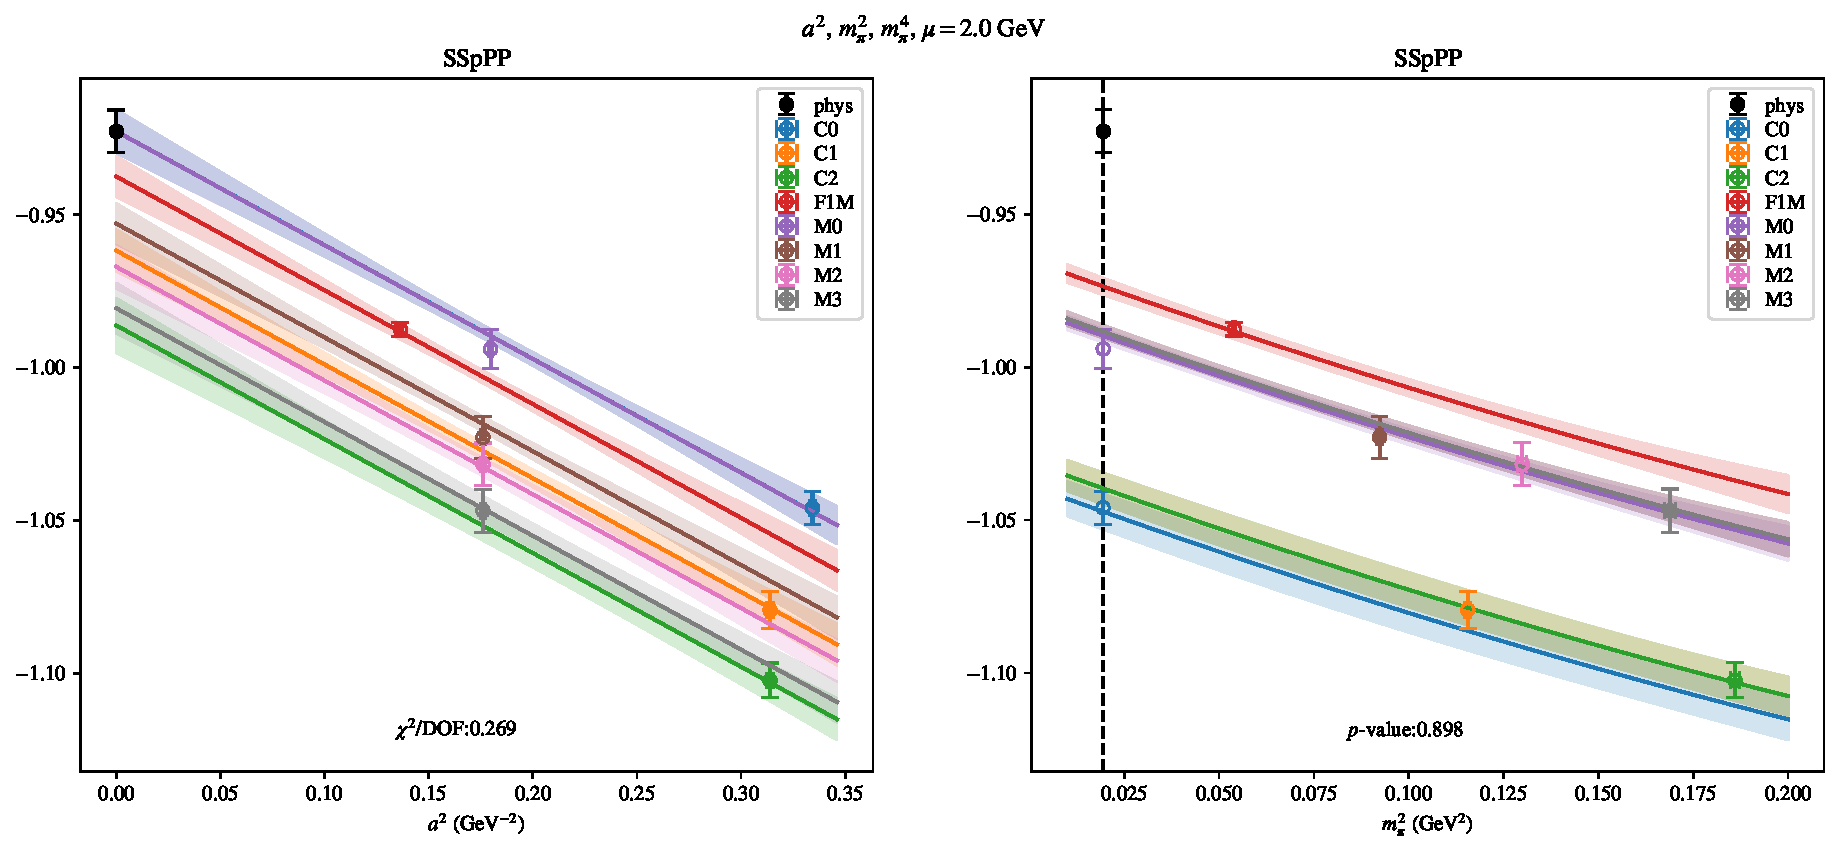
\includepdf[link, pages=-]{VVmAA/SUSY/a2m2m4_20.pdf}
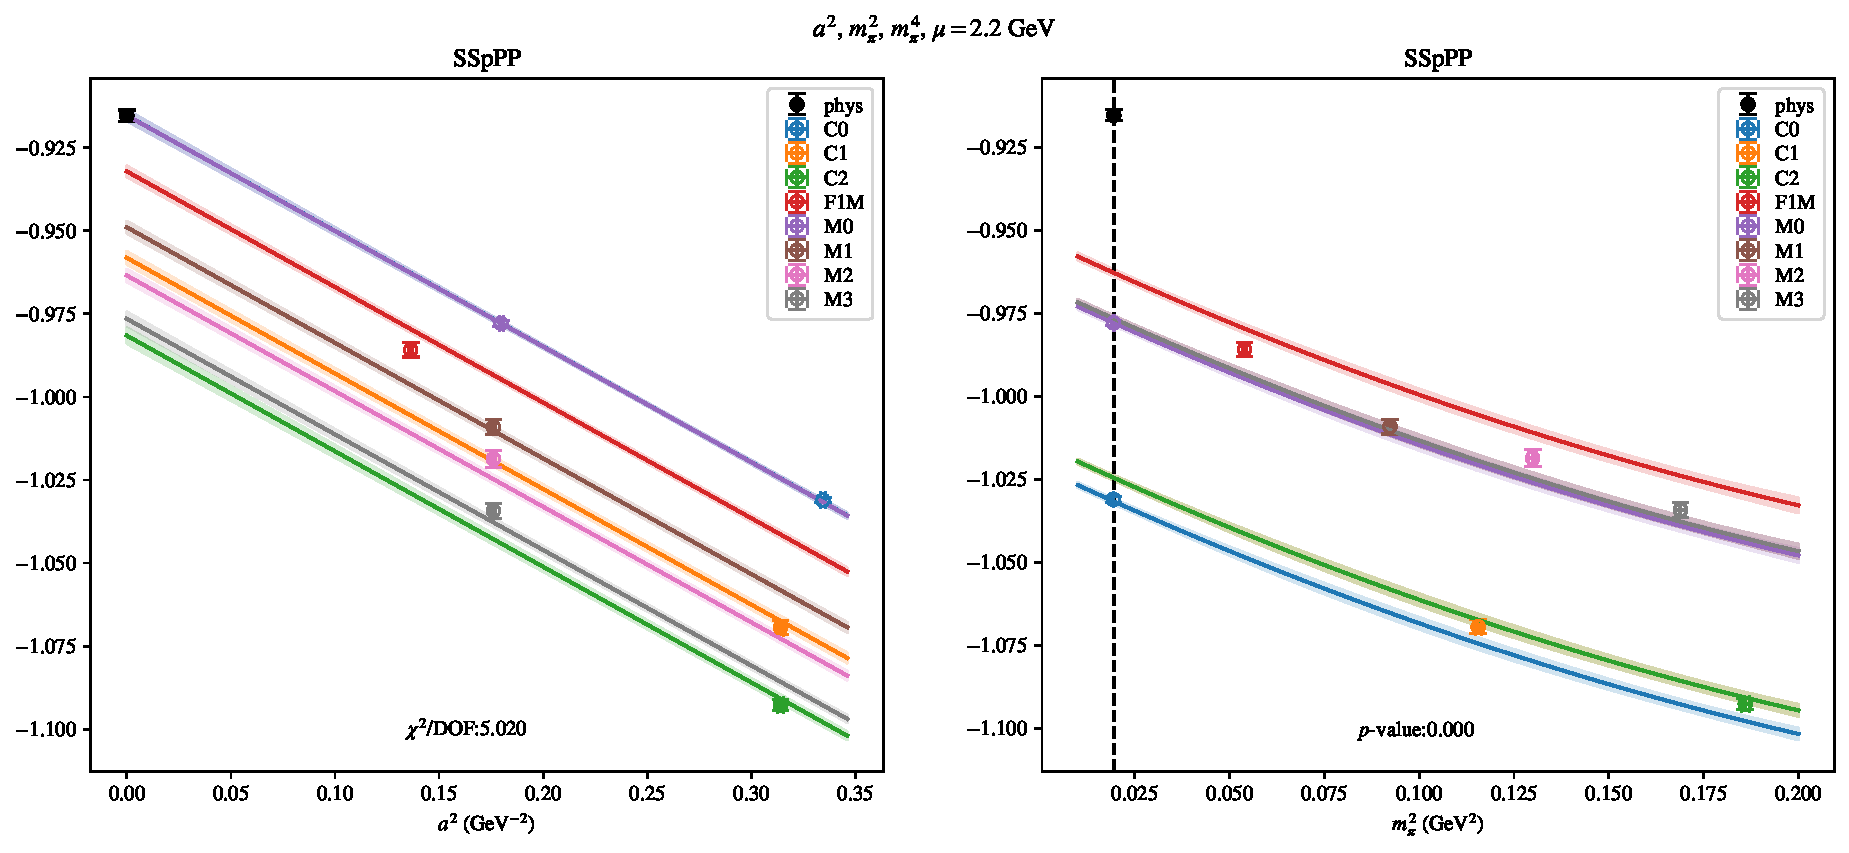
\includepdf[link, pages=-]{VVmAA/SUSY/a2m2m4_22.pdf}
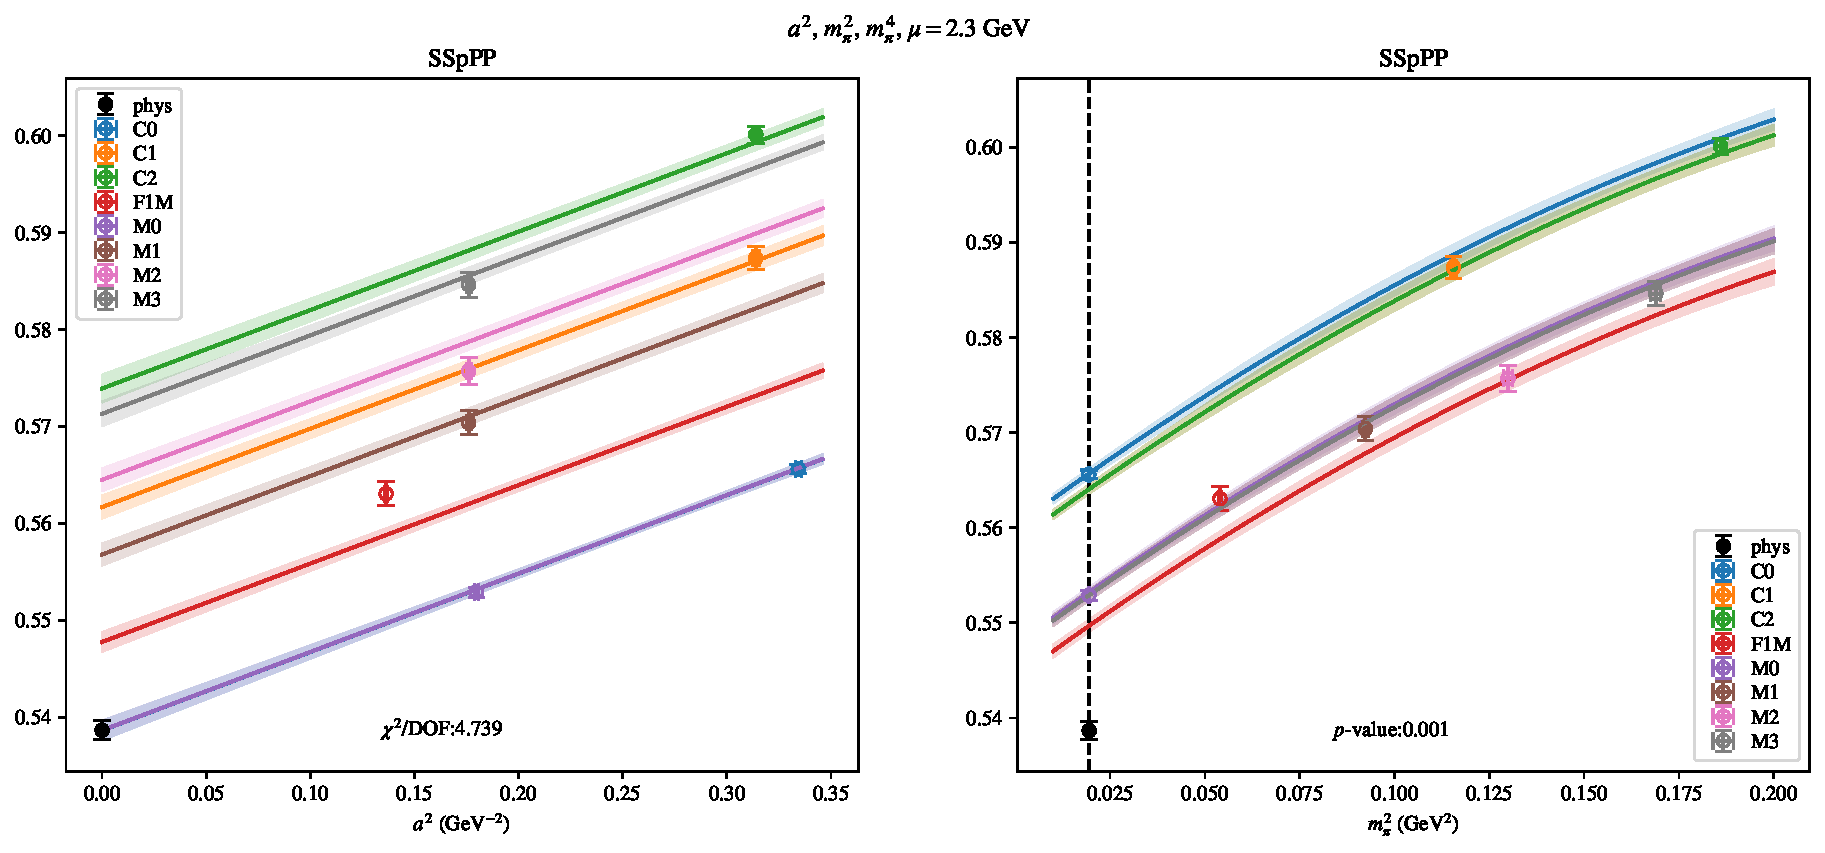
\includepdf[link, pages=-]{VVmAA/SUSY/a2m2m4_23.pdf}
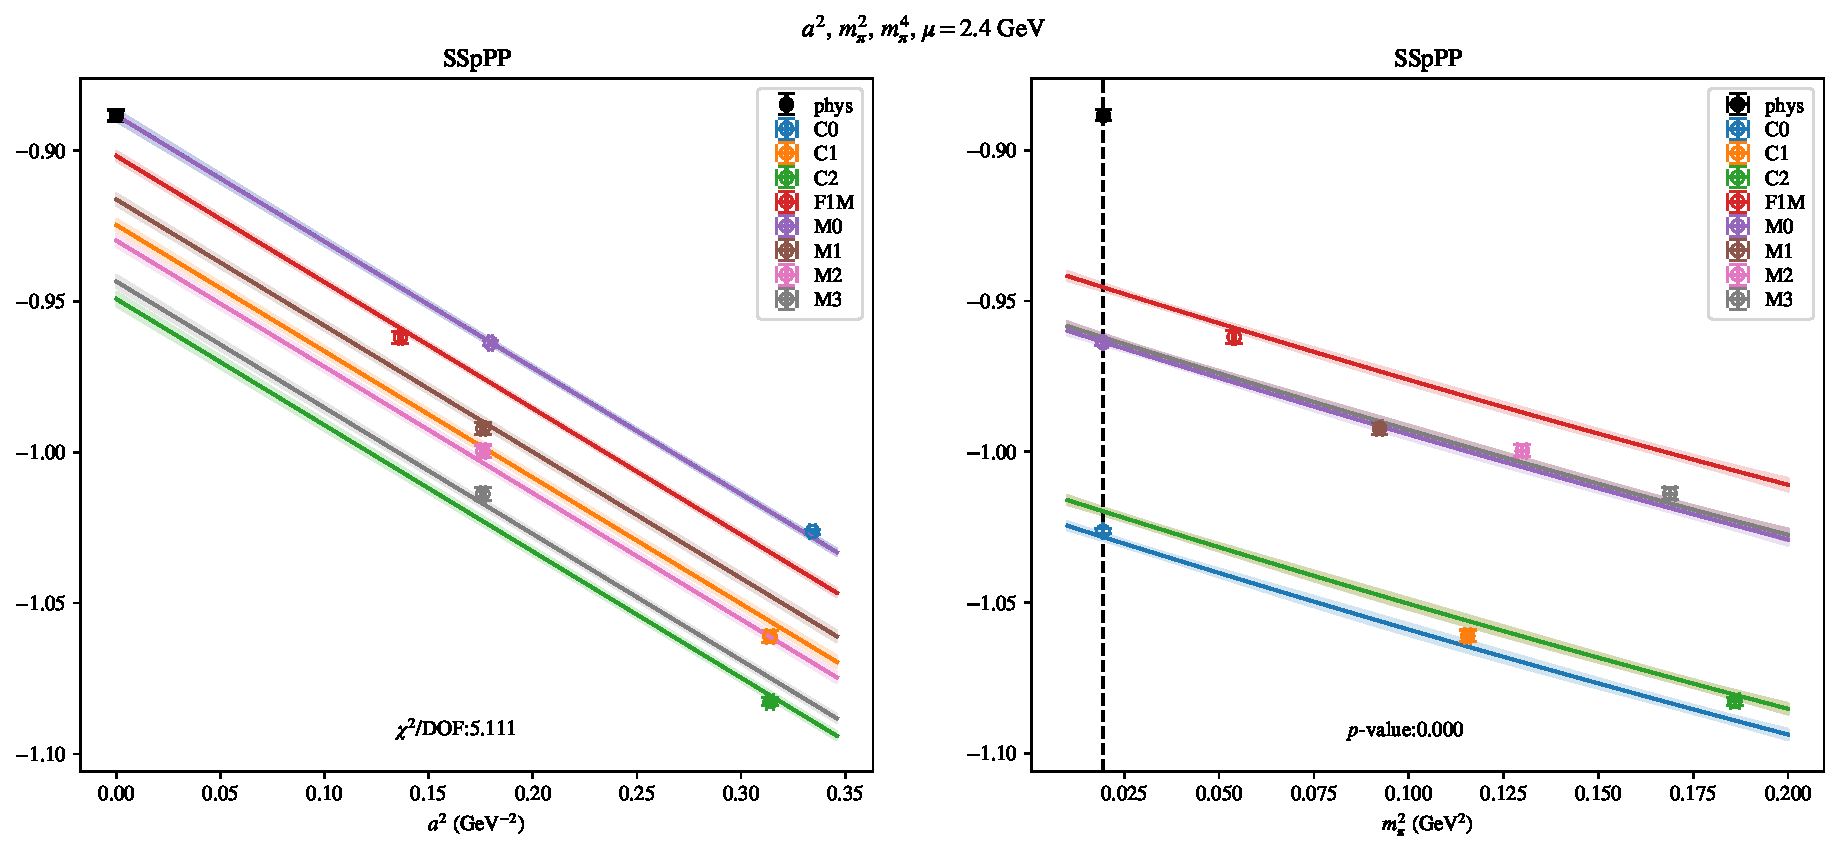
\includepdf[link, pages=-]{VVmAA/SUSY/a2m2m4_24.pdf}
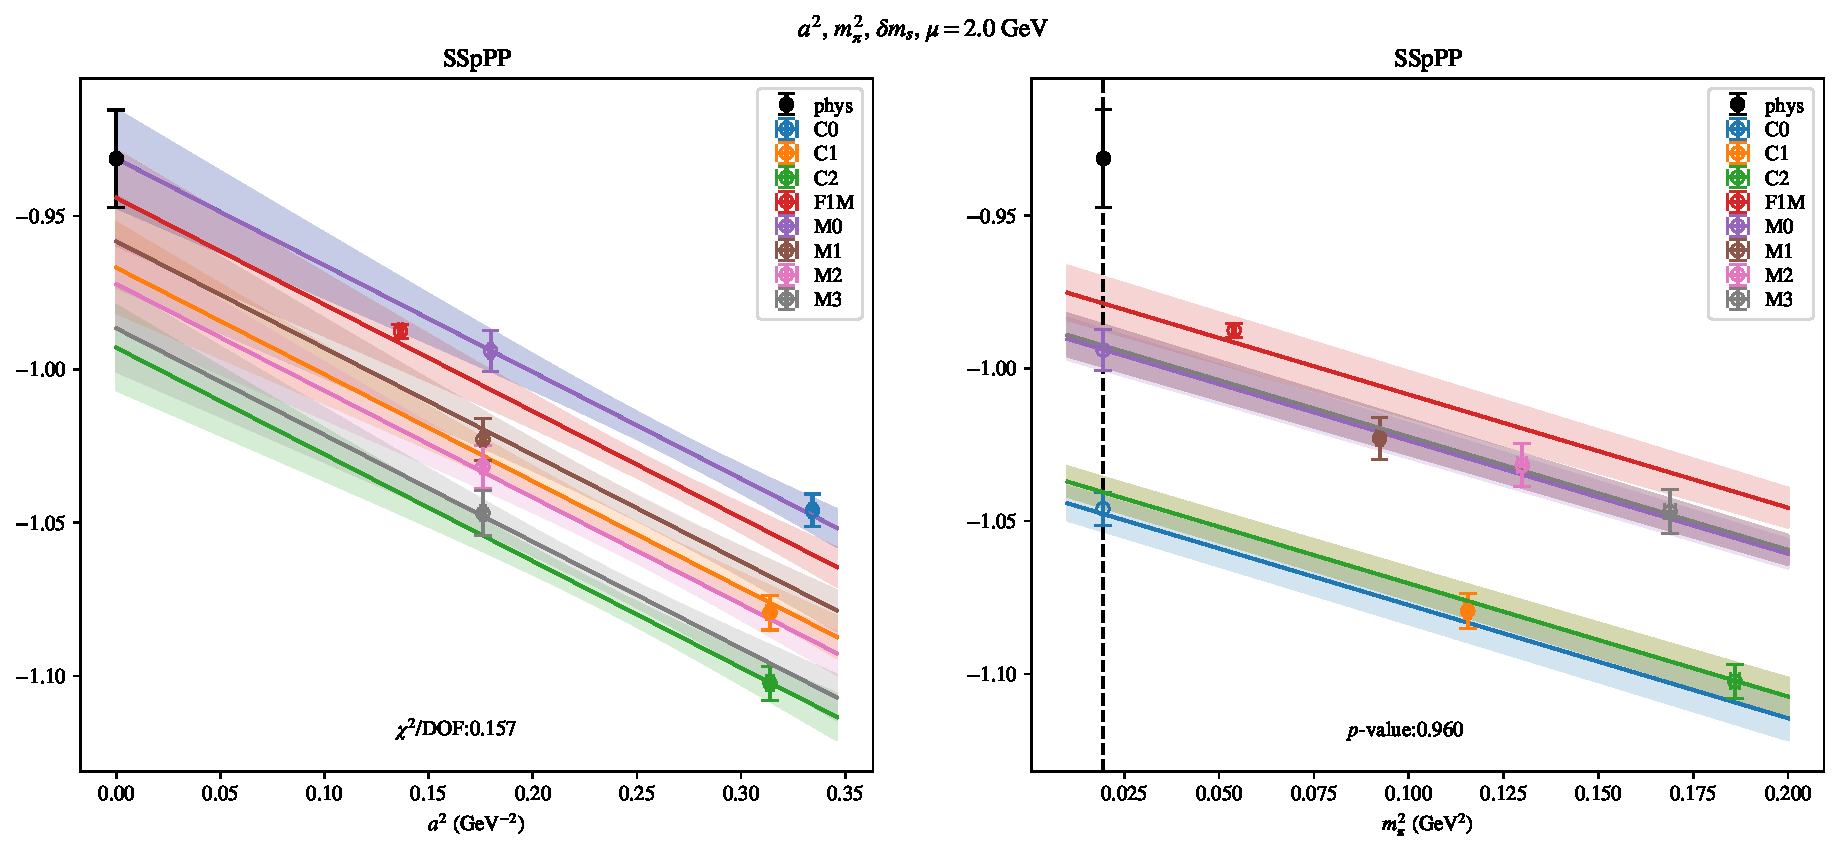
\includepdf[link, pages=-]{VVmAA/SUSY/a2m2delm_20.pdf}
\includepdf[link, pages=-]{VVmAA/SUSY/a2m2delm_22.pdf}
\includepdf[link, pages=-]{VVmAA/SUSY/a2m2delm_23.pdf}
\includepdf[link, pages=-]{VVmAA/SUSY/a2m2delm_24.pdf}
\clearpage
\section{$\mathcal{B}_3$}
\begin{table}[h!]
\begin{center}
\begin{tabular}{|c|c|c|c|c|c|c|}
\hline
$\mu$ (GeV) & $a^2$, $m_\pi^2$& $a^2$, $m_\pi^2$ (no C)& $a^2$, $a^4$, $m_\pi^2$& $a^2$, $m_\pi^2$ (no M3, C2)& $a^2$, $m_\pi^2$, $m_\pi^4$& $a^2$, $m_\pi^2$, $\delta m_s$\\
\hline
2.0& \hyperlink{SSmPP/SUSY/a2m2_20.pdf.1}{\textbf{0.28164(67)}: 4.433 (0.0)} & \hyperlink{SSmPP/SUSY/a2m2noC_20.pdf.1}{\textbf{0.2859(30)}: 4.463 (0.012)} & \hyperlink{SSmPP/SUSY/a2a4m2_20.pdf.1}{\textbf{0.2826(52)}: 5.531 (0.0)} & \hyperlink{SSmPP/SUSY/a2m2mcut_20.pdf.1}{\textbf{0.28157(72)}: 4.725 (0.003)} & \hyperlink{SSmPP/SUSY/a2m2m4_20.pdf.1}{\textbf{0.28095(73)}: 3.752 (0.005)} & \hyperlink{SSmPP/SUSY/a2m2delm_20.pdf.1}{\textbf{0.28141(75)}: 5.331 (0.0)}\\
2.2& \hyperlink{SSmPP/SUSY/a2m2_22.pdf.1}{\textbf{0.27303(66)}: 6.117 (0.0)} & \hyperlink{SSmPP/SUSY/a2m2noC_22.pdf.1}{\textbf{0.2789(28)}: 3.583 (0.028)} & \hyperlink{SSmPP/SUSY/a2a4m2_22.pdf.1}{\textbf{0.2742(51)}: 7.63 (0.0)} & \hyperlink{SSmPP/SUSY/a2m2mcut_22.pdf.1}{\textbf{0.27326(71)}: 5.632 (0.001)} & \hyperlink{SSmPP/SUSY/a2m2m4_22.pdf.1}{\textbf{0.27242(71)}: 5.958 (0.0)} & \hyperlink{SSmPP/SUSY/a2m2delm_22.pdf.1}{\textbf{0.27266(74)}: 7.008 (0.0)}\\
2.3& \hyperlink{SSmPP/SUSY/a2m2_23.pdf.1}{\textbf{0.26918(66)}: 6.811 (0.0)} & \hyperlink{SSmPP/SUSY/a2m2noC_23.pdf.1}{\textbf{0.2760(28)}: 3.885 (0.021)} & \hyperlink{SSmPP/SUSY/a2a4m2_23.pdf.1}{\textbf{0.2716(51)}: 8.436 (0.0)} & \hyperlink{SSmPP/SUSY/a2m2mcut_23.pdf.1}{\textbf{0.26941(72)}: 6.776 (0.0)} & \hyperlink{SSmPP/SUSY/a2m2m4_23.pdf.1}{\textbf{0.26855(72)}: 6.755 (0.0)} & \hyperlink{SSmPP/SUSY/a2m2delm_23.pdf.1}{\textbf{0.26875(75)}: 7.557 (0.0)}\\
2.4& \hyperlink{SSmPP/SUSY/a2m2_24.pdf.1}{\textbf{0.26582(67)}: 7.61 (0.0)} & \hyperlink{SSmPP/SUSY/a2m2noC_24.pdf.1}{\textbf{0.2728(28)}: 3.909 (0.02)} & \hyperlink{SSmPP/SUSY/a2a4m2_24.pdf.1}{\textbf{0.2679(51)}: 9.453 (0.0)} & \hyperlink{SSmPP/SUSY/a2m2mcut_24.pdf.1}{\textbf{0.26611(73)}: 7.937 (0.0)} & \hyperlink{SSmPP/SUSY/a2m2m4_24.pdf.1}{\textbf{0.26523(73)}: 7.981 (0.0)} & \hyperlink{SSmPP/SUSY/a2m2delm_24.pdf.1}{\textbf{0.26538(76)}: 8.448 (0.0)}\\
\hline
\end{tabular}
\caption{Physical point value from chiral and continuum extrapolation at renormalisation scale $\mu$. Entries are \textbf{value(error)}: $\chi^2/\text{DOF}$ ($p$-value).}
\end{center}
\end{table}
\begin{table}[h!]
\begin{center}
\begin{tabular}{|c c|c|c|c|c|c|c|}
\hline
$\mu$ (GeV) &  & $a^2$, $m_\pi^2$& $a^2$, $m_\pi^2$ (no C)& $a^2$, $a^4$, $m_\pi^2$& $a^2$, $m_\pi^2$ (no M3, C2)& $a^2$, $m_\pi^2$, $m_\pi^4$& $a^2$, $m_\pi^2$, $\delta m_s$\\
\hline
\multirow{2}{0.5in}{2.0} & $\alpha$ & 0.642(10)& 0.549(67)& 0.60(18)& 0.642(11)& 0.651(11)& 0.645(11)\\
 & $\beta$ & 0.00696(20)& 0.00632(31)& 0.00694(21)& 0.00753(31)& 0.00949(94)& 0.00701(21)\\
\hline
\multirow{2}{0.5in}{2.2} & $\alpha$ & 0.755(11)& 0.623(66)& 0.71(18)& 0.749(12)& 0.763(12)& 0.760(12)\\
 & $\beta$ & 0.00749(19)& 0.00660(27)& 0.00748(22)& 0.00809(31)& 0.00986(92)& 0.00758(21)\\
\hline
\multirow{2}{0.5in}{2.3} & $\alpha$ & 0.810(11)& 0.655(67)& 0.72(18)& 0.805(12)& 0.820(12)& 0.817(12)\\
 & $\beta$ & 0.00766(20)& 0.00672(25)& 0.00762(22)& 0.00821(31)& 0.01002(93)& 0.00777(21)\\
\hline
\multirow{2}{0.5in}{2.4} & $\alpha$ & 0.862(12)& 0.700(67)& 0.78(19)& 0.856(13)& 0.871(13)& 0.869(13)\\
 & $\beta$ & 0.00785(20)& 0.00683(25)& 0.00781(23)& 0.00831(31)& 0.01003(94)& 0.00797(22)\\
\hline
\end{tabular}
\caption{Fit values of coefficients in $Q = Q_{phys} + \mathbf{\alpha} a^2 + \mathbf{\beta}\left(\frac{m_\pi^2}{f_\pi^2}-\frac{m_{\pi,PDG}^2}{f_\pi^2}\right) + \ldots$.}
\end{center}
\end{table}
\includepdf[link, pages=-]{SSmPP/SUSY/a2m2_20.pdf}
\includepdf[link, pages=-]{SSmPP/SUSY/a2m2_22.pdf}
\includepdf[link, pages=-]{SSmPP/SUSY/a2m2_23.pdf}
\includepdf[link, pages=-]{SSmPP/SUSY/a2m2_24.pdf}
\includepdf[link, pages=-]{SSmPP/SUSY/a2m2noC_20.pdf}
\includepdf[link, pages=-]{SSmPP/SUSY/a2m2noC_22.pdf}
\includepdf[link, pages=-]{SSmPP/SUSY/a2m2noC_23.pdf}
\includepdf[link, pages=-]{SSmPP/SUSY/a2m2noC_24.pdf}
\includepdf[link, pages=-]{SSmPP/SUSY/a2a4m2_20.pdf}
\includepdf[link, pages=-]{SSmPP/SUSY/a2a4m2_22.pdf}
\includepdf[link, pages=-]{SSmPP/SUSY/a2a4m2_23.pdf}
\includepdf[link, pages=-]{SSmPP/SUSY/a2a4m2_24.pdf}
\includepdf[link, pages=-]{SSmPP/SUSY/a2m2mcut_20.pdf}
\includepdf[link, pages=-]{SSmPP/SUSY/a2m2mcut_22.pdf}
\includepdf[link, pages=-]{SSmPP/SUSY/a2m2mcut_23.pdf}
\includepdf[link, pages=-]{SSmPP/SUSY/a2m2mcut_24.pdf}
\includepdf[link, pages=-]{SSmPP/SUSY/a2m2m4_20.pdf}
\includepdf[link, pages=-]{SSmPP/SUSY/a2m2m4_22.pdf}
\includepdf[link, pages=-]{SSmPP/SUSY/a2m2m4_23.pdf}
\includepdf[link, pages=-]{SSmPP/SUSY/a2m2m4_24.pdf}
\includepdf[link, pages=-]{SSmPP/SUSY/a2m2delm_20.pdf}
\includepdf[link, pages=-]{SSmPP/SUSY/a2m2delm_22.pdf}
\includepdf[link, pages=-]{SSmPP/SUSY/a2m2delm_23.pdf}
\includepdf[link, pages=-]{SSmPP/SUSY/a2m2delm_24.pdf}
\clearpage
\section{$\mathcal{B}_4$}
\begin{table}[h!]
\begin{center}
\begin{tabular}{|c|c|c|c|c|c|c|}
\hline
$\mu$ (GeV) & $a^2$, $m_\pi^2$& $a^2$, $m_\pi^2$ (no C)& $a^2$, $a^4$, $m_\pi^2$& $a^2$, $m_\pi^2$ (no M3, C2)& $a^2$, $m_\pi^2$, $m_\pi^4$& $a^2$, $m_\pi^2$, $\delta m_s$\\
\hline
2.0& \hyperlink{SSpPP/SUSY/a2m2_20.pdf.1}{\textbf{1.8001(27)}: 16.344 (0.0)} & \hyperlink{SSpPP/SUSY/a2m2noC_20.pdf.1}{\textbf{1.692(13)}: 0.633 (0.531)} & \hyperlink{SSpPP/SUSY/a2a4m2_20.pdf.1}{\textbf{1.622(20)}: 1.014 (0.399)} & \hyperlink{SSpPP/SUSY/a2m2mcut_20.pdf.1}{\textbf{1.8014(27)}: 25.726 (0.0)} & \hyperlink{SSpPP/SUSY/a2m2m4_20.pdf.1}{\textbf{1.8052(28)}: 15.706 (0.0)} & \hyperlink{SSpPP/SUSY/a2m2delm_20.pdf.1}{\textbf{1.8111(29)}: 1.395 (0.233)}\\
2.2& \hyperlink{SSpPP/SUSY/a2m2_22.pdf.1}{\textbf{1.8057(26)}: 15.08 (0.0)} & \hyperlink{SSpPP/SUSY/a2m2noC_22.pdf.1}{\textbf{1.705(12)}: 1.335 (0.263)} & \hyperlink{SSpPP/SUSY/a2a4m2_22.pdf.1}{\textbf{1.639(20)}: 1.482 (0.205)} & \hyperlink{SSpPP/SUSY/a2m2mcut_22.pdf.1}{\textbf{1.8071(27)}: 22.642 (0.0)} & \hyperlink{SSpPP/SUSY/a2m2m4_22.pdf.1}{\textbf{1.8108(27)}: 13.617 (0.0)} & \hyperlink{SSpPP/SUSY/a2m2delm_22.pdf.1}{\textbf{1.8156(28)}: 2.284 (0.058)}\\
2.3& \hyperlink{SSpPP/SUSY/a2m2_23.pdf.1}{\textbf{1.8080(25)}: 14.417 (0.0)} & \hyperlink{SSpPP/SUSY/a2m2noC_23.pdf.1}{\textbf{1.709(12)}: 1.489 (0.226)} & \hyperlink{SSpPP/SUSY/a2a4m2_23.pdf.1}{\textbf{1.644(20)}: 1.379 (0.238)} & \hyperlink{SSpPP/SUSY/a2m2mcut_23.pdf.1}{\textbf{1.8093(27)}: 21.872 (0.0)} & \hyperlink{SSpPP/SUSY/a2m2m4_23.pdf.1}{\textbf{1.8130(27)}: 13.368 (0.0)} & \hyperlink{SSpPP/SUSY/a2m2delm_23.pdf.1}{\textbf{1.8175(27)}: 2.373 (0.05)}\\
2.4& \hyperlink{SSpPP/SUSY/a2m2_24.pdf.1}{\textbf{1.8094(25)}: 13.33 (0.0)} & \hyperlink{SSpPP/SUSY/a2m2noC_24.pdf.1}{\textbf{1.714(12)}: 1.494 (0.224)} & \hyperlink{SSpPP/SUSY/a2a4m2_24.pdf.1}{\textbf{1.652(20)}: 1.366 (0.243)} & \hyperlink{SSpPP/SUSY/a2m2mcut_24.pdf.1}{\textbf{1.8106(27)}: 20.362 (0.0)} & \hyperlink{SSpPP/SUSY/a2m2m4_24.pdf.1}{\textbf{1.8142(27)}: 12.58 (0.0)} & \hyperlink{SSpPP/SUSY/a2m2delm_24.pdf.1}{\textbf{1.8183(27)}: 2.277 (0.058)}\\
\hline
\end{tabular}
\caption{Physical point value from chiral and continuum extrapolation at renormalisation scale $\mu$. Entries are \textbf{value(error)}: $\chi^2/\text{DOF}$ ($p$-value).}
\end{center}
\end{table}
\begin{table}[h!]
\begin{center}
\begin{tabular}{|c c|c|c|c|c|c|c|}
\hline
$\mu$ (GeV) &  & $a^2$, $m_\pi^2$& $a^2$, $m_\pi^2$ (no C)& $a^2$, $a^4$, $m_\pi^2$& $a^2$, $m_\pi^2$ (no M3, C2)& $a^2$, $m_\pi^2$, $m_\pi^4$& $a^2$, $m_\pi^2$, $\delta m_s$\\
\hline
\multirow{2}{0.5in}{2.0} & $\alpha$ & 0.0704(58)& 0.446(47)& 1.06(12)& 0.0682(59)& 0.0610(61)& 0.0495(61)\\
 & $\beta$ & -0.0011(13)& -0.0011(27)& -0.0015(15)& -0.0015(24)& -0.0041(71)& -0.0013(13)\\
\hline
\multirow{2}{0.5in}{2.2} & $\alpha$ & 0.0760(55)& 0.425(46)& 0.99(12)& 0.0739(58)& 0.0667(58)& 0.0573(59)\\
 & $\beta$ & -0.0007(12)& -0.0008(24)& -0.0011(14)& -0.0012(23)& -0.0037(66)& -0.0009(12)\\
\hline
\multirow{2}{0.5in}{2.3} & $\alpha$ & 0.0772(54)& 0.417(45)& 0.97(12)& 0.0752(58)& 0.0681(58)& 0.0594(58)\\
 & $\beta$ & -0.0007(12)& -0.0008(23)& -0.0011(14)& -0.0011(23)& -0.0034(65)& -0.0009(11)\\
\hline
\multirow{2}{0.5in}{2.4} & $\alpha$ & 0.0790(54)& 0.406(45)& 0.93(12)& 0.0772(58)& 0.0702(58)& 0.0624(57)\\
 & $\beta$ & -0.0006(11)& -0.0007(22)& -0.0010(13)& -0.0010(22)& -0.0032(63)& -0.0008(11)\\
\hline
\end{tabular}
\caption{Fit values of coefficients in $Q = Q_{phys} + \mathbf{\alpha} a^2 + \mathbf{\beta}\left(\frac{m_\pi^2}{f_\pi^2}-\frac{m_{\pi,PDG}^2}{f_\pi^2}\right) + \ldots$.}
\end{center}
\end{table}
\includepdf[link, pages=-]{SSpPP/SUSY/a2m2_20.pdf}
\includepdf[link, pages=-]{SSpPP/SUSY/a2m2_22.pdf}
\includepdf[link, pages=-]{SSpPP/SUSY/a2m2_23.pdf}
\includepdf[link, pages=-]{SSpPP/SUSY/a2m2_24.pdf}
\includepdf[link, pages=-]{SSpPP/SUSY/a2m2noC_20.pdf}
\includepdf[link, pages=-]{SSpPP/SUSY/a2m2noC_22.pdf}
\includepdf[link, pages=-]{SSpPP/SUSY/a2m2noC_23.pdf}
\includepdf[link, pages=-]{SSpPP/SUSY/a2m2noC_24.pdf}
\includepdf[link, pages=-]{SSpPP/SUSY/a2a4m2_20.pdf}
\includepdf[link, pages=-]{SSpPP/SUSY/a2a4m2_22.pdf}
\includepdf[link, pages=-]{SSpPP/SUSY/a2a4m2_23.pdf}
\includepdf[link, pages=-]{SSpPP/SUSY/a2a4m2_24.pdf}
\includepdf[link, pages=-]{SSpPP/SUSY/a2m2mcut_20.pdf}
\includepdf[link, pages=-]{SSpPP/SUSY/a2m2mcut_22.pdf}
\includepdf[link, pages=-]{SSpPP/SUSY/a2m2mcut_23.pdf}
\includepdf[link, pages=-]{SSpPP/SUSY/a2m2mcut_24.pdf}
\includepdf[link, pages=-]{SSpPP/SUSY/a2m2m4_20.pdf}
\includepdf[link, pages=-]{SSpPP/SUSY/a2m2m4_22.pdf}
\includepdf[link, pages=-]{SSpPP/SUSY/a2m2m4_23.pdf}
\includepdf[link, pages=-]{SSpPP/SUSY/a2m2m4_24.pdf}
\includepdf[link, pages=-]{SSpPP/SUSY/a2m2delm_20.pdf}
\includepdf[link, pages=-]{SSpPP/SUSY/a2m2delm_22.pdf}
\includepdf[link, pages=-]{SSpPP/SUSY/a2m2delm_23.pdf}
\includepdf[link, pages=-]{SSpPP/SUSY/a2m2delm_24.pdf}
\clearpage
\section{$\mathcal{B}_5$}
\begin{table}[h!]
\begin{center}
\begin{tabular}{|c|c|c|c|c|c|c|}
\hline
$\mu$ (GeV) & $a^2$, $m_\pi^2$& $a^2$, $m_\pi^2$ (no C)& $a^2$, $a^4$, $m_\pi^2$& $a^2$, $m_\pi^2$ (no M3, C2)& $a^2$, $m_\pi^2$, $m_\pi^4$& $a^2$, $m_\pi^2$, $\delta m_s$\\
\hline
2.0& \hyperlink{TT/SUSY/a2m2_20.pdf.1}{\textbf{0.49596(77)}: 10.937 (0.0)} & \hyperlink{TT/SUSY/a2m2noC_20.pdf.1}{\textbf{0.4656(44)}: 1.835 (0.16)} & \hyperlink{TT/SUSY/a2a4m2_20.pdf.1}{\textbf{0.4489(66)}: 1.828 (0.12)} & \hyperlink{TT/SUSY/a2m2mcut_20.pdf.1}{\textbf{0.49622(77)}: 17.076 (0.0)} & \hyperlink{TT/SUSY/a2m2m4_20.pdf.1}{\textbf{0.49685(78)}: 10.401 (0.0)} & \hyperlink{TT/SUSY/a2m2delm_20.pdf.1}{\textbf{0.49769(83)}: 2.103 (0.078)}\\
2.2& \hyperlink{TT/SUSY/a2m2_22.pdf.1}{\textbf{0.50299(74)}: 10.281 (0.0)} & \hyperlink{TT/SUSY/a2m2noC_22.pdf.1}{\textbf{0.4750(43)}: 2.906 (0.055)} & \hyperlink{TT/SUSY/a2a4m2_22.pdf.1}{\textbf{0.4600(67)}: 2.562 (0.036)} & \hyperlink{TT/SUSY/a2m2mcut_22.pdf.1}{\textbf{0.50329(75)}: 14.538 (0.0)} & \hyperlink{TT/SUSY/a2m2m4_22.pdf.1}{\textbf{0.50396(76)}: 8.697 (0.0)} & \hyperlink{TT/SUSY/a2m2delm_22.pdf.1}{\textbf{0.50447(80)}: 3.216 (0.012)}\\
2.3& \hyperlink{TT/SUSY/a2m2_23.pdf.1}{\textbf{0.50609(74)}: 10.305 (0.0)} & \hyperlink{TT/SUSY/a2m2noC_23.pdf.1}{\textbf{0.4784(43)}: 3.09 (0.046)} & \hyperlink{TT/SUSY/a2a4m2_23.pdf.1}{\textbf{0.4632(66)}: 2.437 (0.045)} & \hyperlink{TT/SUSY/a2m2mcut_23.pdf.1}{\textbf{0.50637(76)}: 14.776 (0.0)} & \hyperlink{TT/SUSY/a2m2m4_23.pdf.1}{\textbf{0.50706(76)}: 9.052 (0.0)} & \hyperlink{TT/SUSY/a2m2delm_23.pdf.1}{\textbf{0.50754(80)}: 3.282 (0.011)}\\
2.4& \hyperlink{TT/SUSY/a2m2_24.pdf.1}{\textbf{0.50842(74)}: 9.408 (0.0)} & \hyperlink{TT/SUSY/a2m2noC_24.pdf.1}{\textbf{0.4821(42)}: 3.081 (0.046)} & \hyperlink{TT/SUSY/a2a4m2_24.pdf.1}{\textbf{0.4687(66)}: 2.619 (0.033)} & \hyperlink{TT/SUSY/a2m2mcut_24.pdf.1}{\textbf{0.50863(77)}: 13.353 (0.0)} & \hyperlink{TT/SUSY/a2m2m4_24.pdf.1}{\textbf{0.50937(77)}: 8.359 (0.0)} & \hyperlink{TT/SUSY/a2m2delm_24.pdf.1}{\textbf{0.50979(81)}: 3.011 (0.017)}\\
\hline
\end{tabular}
\caption{Physical point value from chiral and continuum extrapolation at renormalisation scale $\mu$. Entries are \textbf{value(error)}: $\chi^2/\text{DOF}$ ($p$-value).}
\end{center}
\end{table}
\begin{table}[h!]
\begin{center}
\begin{tabular}{|c c|c|c|c|c|c|c|}
\hline
$\mu$ (GeV) &  & $a^2$, $m_\pi^2$& $a^2$, $m_\pi^2$ (no C)& $a^2$, $a^4$, $m_\pi^2$& $a^2$, $m_\pi^2$ (no M3, C2)& $a^2$, $m_\pi^2$, $m_\pi^4$& $a^2$, $m_\pi^2$, $\delta m_s$\\
\hline
\multirow{2}{0.5in}{2.0} & $\alpha$ & -0.184(55)& 0.176(56)& 0.72(14)& -0.185(55)& -0.189(56)& -0.195(59)\\
 & $\beta$ & 0.00104(14)& 0.00114(26)& 0.00085(17)& 0.00068(24)& -0.0015(76)& 0.00081(14)\\
\hline
\multirow{2}{0.5in}{2.2} & $\alpha$ & -0.224(53)& 0.099(53)& 0.58(13)& -0.225(53)& -0.230(53)& -0.233(56)\\
 & $\beta$ & 0.00115(13)& 0.00119(23)& 0.00097(15)& 0.00065(22)& -0.0014(70)& 0.00094(13)\\
\hline
\multirow{2}{0.5in}{2.3} & $\alpha$ & -0.246(52)& 0.070(52)& 0.54(13)& -0.247(53)& -0.252(53)& -0.255(56)\\
 & $\beta$ & 0.00116(12)& 0.00119(22)& 0.00098(15)& 0.00070(21)& -0.0012(68)& 0.00094(13)\\
\hline
\multirow{2}{0.5in}{2.4} & $\alpha$ & -0.265(52)& 0.031(50)& 0.46(13)& -0.266(54)& -0.271(53)& -0.274(56)\\
 & $\beta$ & 0.00112(12)& 0.00120(20)& 0.00095(14)& 0.00069(21)& -0.0011(67)& 0.00091(13)\\
\hline
\end{tabular}
\caption{Fit values of coefficients in $Q = Q_{phys} + \mathbf{\alpha} a^2 + \mathbf{\beta}\left(\frac{m_\pi^2}{f_\pi^2}-\frac{m_{\pi,PDG}^2}{f_\pi^2}\right) + \ldots$.}
\end{center}
\end{table}
\includepdf[link, pages=-]{TT/SUSY/a2m2_20.pdf}
\includepdf[link, pages=-]{TT/SUSY/a2m2_22.pdf}
\includepdf[link, pages=-]{TT/SUSY/a2m2_23.pdf}
\includepdf[link, pages=-]{TT/SUSY/a2m2_24.pdf}
\includepdf[link, pages=-]{TT/SUSY/a2m2noC_20.pdf}
\includepdf[link, pages=-]{TT/SUSY/a2m2noC_22.pdf}
\includepdf[link, pages=-]{TT/SUSY/a2m2noC_23.pdf}
\includepdf[link, pages=-]{TT/SUSY/a2m2noC_24.pdf}
\includepdf[link, pages=-]{TT/SUSY/a2a4m2_20.pdf}
\includepdf[link, pages=-]{TT/SUSY/a2a4m2_22.pdf}
\includepdf[link, pages=-]{TT/SUSY/a2a4m2_23.pdf}
\includepdf[link, pages=-]{TT/SUSY/a2a4m2_24.pdf}
\includepdf[link, pages=-]{TT/SUSY/a2m2mcut_20.pdf}
\includepdf[link, pages=-]{TT/SUSY/a2m2mcut_22.pdf}
\includepdf[link, pages=-]{TT/SUSY/a2m2mcut_23.pdf}
\includepdf[link, pages=-]{TT/SUSY/a2m2mcut_24.pdf}
\includepdf[link, pages=-]{TT/SUSY/a2m2m4_20.pdf}
\includepdf[link, pages=-]{TT/SUSY/a2m2m4_22.pdf}
\includepdf[link, pages=-]{TT/SUSY/a2m2m4_23.pdf}
\includepdf[link, pages=-]{TT/SUSY/a2m2m4_24.pdf}
\includepdf[link, pages=-]{TT/SUSY/a2m2delm_20.pdf}
\includepdf[link, pages=-]{TT/SUSY/a2m2delm_22.pdf}
\includepdf[link, pages=-]{TT/SUSY/a2m2delm_23.pdf}
\includepdf[link, pages=-]{TT/SUSY/a2m2delm_24.pdf}
\clearpage
\end{document}